% !TEX TS-program = lualatex
\documentclass[a4paper,12pt,twoside,extrafontsizes]{memoir}

% This file is automatically generated by the build system.
% Do not edit it manually.

\newcommand{\productversion}{1.0.6}

\usepackage{microtype}
\usepackage{alltt}
\usepackage{enumitem}
\usepackage{multirow}
\usepackage{amsmath}
\usepackage{needspace}
\usepackage{longtable}

\usepackage{tcolorbox}
\tcbuselibrary{breakable}

\usepackage{fontspec}
\setmainfont[Ligatures=TeX]{XCharter}
\setmonofont[Scale=MatchLowercase]{DejaVu Sans Mono}

\usepackage[english]{babel}

\usepackage{listings}
\lstset{breaklines,breakatwhitespace,showstringspaces=false}

\usepackage{perpage}
\MakePerPage{footnote}

\newcommand{\styledtitleref}[1]{\emph{\titleref{#1}}}
\newcommand{\lscaps}[1]{\textls[25]{\MakeTextUppercase{\textit{#1}}}}

\newlength{\baseparindent}
\setlength{\baseparindent}{\parindent}

%%%%%%%%%%%%%%%%%%%%%%%%%%%%%%%%%%
% Various Memoir class settings
%%%%%%%%%%%%%%%%%%%%%%%%%%%%%%%%%%

\sloppybottom
\setsecnumdepth{subsection}

\makeevenhead{headings}{\thepage}{}{\itshape\lscaps{\leftmark}}
\makeoddhead{headings}{\itshape\lscaps{\rightmark}}{}{\thepage}

\setpnumwidth{2.55em}
\setrmarg{3.55em}

%%%%%%%%%%%%%%%%%%%%%%%%%%%%%%%%%%
% Shell commands
%%%%%%%%%%%%%%%%%%%%%%%%%%%%%%%%%%

\newcommand{\shellcmd}[1]{\texttt{#1}}
\newcommand{\smallshellcmd}[1]{\small\texttt{#1}}

\newenvironment{shellcmds}{%
	\vspace{0.5\baselineskip}\begin{tcolorbox}[fontupper=\footnotesize]\begin{alltt}%
}{%
	\end{alltt}\end{tcolorbox}\vspace{0.5\baselineskip}%
}

\newenvironment{breakshellcmds}{%
	\vspace{0.5\baselineskip}\begin{tcolorbox}[fontupper=\footnotesize,breakable]\begin{alltt}%
		}{%
	\end{alltt}\end{tcolorbox}\vspace{0.5\baselineskip}%
}

\newenvironment{breakshellcmdsnamed}[1]{%
	\vspace{0.5\baselineskip}\begin{tcolorbox}[fontupper=\footnotesize,breakable,title=#1]\begin{alltt}%
		}{%
	\end{alltt}\end{tcolorbox}\vspace{0.5\baselineskip}%
}

%%%%%%%%%%%%%%%%%%%%%%%%%%%%%%%%%%
% Progam elements
%%%%%%%%%%%%%%%%%%%%%%%%%%%%%%%%%%

\newcommand{\uielement}[1]{\emph{#1}}

%%%%%%%%%%%%%%%%%%%%%%%%%%%%%%%%%%
% Tables
%%%%%%%%%%%%%%%%%%%%%%%%%%%%%%%%%%

\newcolumntype{L}{>{\raggedright\arraybackslash}X}
\newcolumntype{R}{>{\raggedleft\arraybackslash}X}
\newcolumntype{C}{>{\centering\arraybackslash}X}

\newcolumntype{Q}[1]{>{\raggedright\arraybackslash}p{#1}}
\newcolumntype{E}[1]{>{\raggedleft\arraybackslash}p{#1}}
\newcolumntype{W}[1]{>{\centering\arraybackslash}p{#1}}

\newcommand{\tabcutin}[2]{\multicolumn{#1}{c}{\emph{#2}}}

% Declare esktlongtable environment

\RequirePackage{longtable}
\RequirePackage{caption}

\setlength\LTleft{0pt}
\setlength\LTright{0pt}

\DeclareCaptionLabelFormat{onlynumber}{#2}
\DeclareCaptionFormat{conttable}{Continuation of the Table #1}

\newenvironment{eskdlongtable}[4]{%
	\noindent\begin{longtable}{@{\extracolsep{\fill}}#1}
	\ifx \\#3\\ \else \label{#3}\\ \fi%
	\caption{#2}\\
	\toprule
	#4\\
	\midrule\endfirsthead
	\captionsetup{labelformat=onlynumber,format=conttable}\caption[]{#2}\\
	\toprule
	#4\\
	\midrule\endhead
}{%
	\end{longtable}
}

%%%%%%%%%%%%%%%%%%%%%%%%%%%%%%%%%%
% Code
%%%%%%%%%%%%%%%%%%%%%%%%%%%%%%%%%%

\newcommand{\expr}[1]{\texttt{#1}}
\newcommand{\cexpr}[1]{\texttt{\lstinline[language=C++]`#1`}}
\newcommand{\luaexpr}[1]{\texttt{\lstinline[language={[5.2]Lua}]`#1`}}

\lstnewenvironment{ccode}{\lstset{language=C++}\ttfamily}{}
\lstnewenvironment{luacode}{\lstset{language=[5.2]Lua}\ttfamily}{}

\newcommand{\objtype}[1]{\emph{#1}}
\newcommand{\luatype}[1]{\emph{#1}}

% Function description

\newlength{\funcparskip}
\setlength{\funcparskip}{0.5\baselineskip}

\lstnewenvironment{cfuncprototype}{%
	\needspace{4\baselineskip}
	\lstset{language=C++,aboveskip=1\funcparskip,belowskip=2\funcparskip,basicstyle=\ttfamily}%
}{}

\newenvironment{luafuncprototype}{
	\par\vspace{0.5\funcparskip}%
	\ttfamily\bfseries\noindent\raggedright\ignorespaces%
}{%
	\par\nopagebreak%
	\vspace{1.5\funcparskip}\nopagebreak
}

\newenvironment{funcdescr}
{\setlength{\parindent}{0pt}}
{\par\vspace{\funcparskip}}

\newcommand{\funcparam}[1]{\item\expr{#1}}

\newenvironment{funcparams}{%
	\noindent \emph{Parameters}:\par\nopagebreak%
	\vspace{0.5\funcparskip}\nopagebreak%
	\begin{itemize}[topsep=0pt,partopsep=0pt,parsep=0pt,itemsep=0.25\funcparskip,label=,leftmargin=\parindent]
}{%
	\end{itemize}
	\par\vspace{\funcparskip}
}

\newenvironment{funcret}{%
	\noindent \emph{Return value}:\par\nopagebreak%
	\vspace{0.5\funcparskip}\nopagebreak%
}{%
	\par\vspace{\funcparskip}
}

\newenvironment{funcremarks}{%
	\noindent \emph{Remarks}:\par\nopagebreak%
	\vspace{0.5\funcparskip}\nopagebreak%
}{%
	\par\vspace{\funcparskip}
}

\newenvironment{funcexamples}{%
	\noindent \emph{Examples}:\par\nopagebreak%
	\vspace{0.5\funcparskip}\nopagebreak%
}{%
	\par\vspace{\funcparskip}
}

%%%%%%%%%%%%%%%%%%%%%%%%%%%%%%%%%%
% Various stuff
%%%%%%%%%%%%%%%%%%%%%%%%%%%%%%%%%%

\newcommand{\cplusplus}{C\texttt{\raisebox{0.05em}{++}}}

\newcommand{\tocitem}[2]{\phantomsection\addcontentsline{toc}{#1}{#2}}

%%%%%%%%%%%%%%%%%%%%%%%%%%%%%%%%%%
% Hyperlinks
%%%%%%%%%%%%%%%%%%%%%%%%%%%%%%%%%%

\usepackage[bookmarks=true,
	bookmarksnumbered=true,
	bookmarksdepth=3,
	hypertexnames=false]
	{hyperref}


\hypersetup{
	pdftitle={Simple Device Model User Manual},
	pdfauthor={Simple Device Model contributors}
}

\begin{document}

\begin{titlingpage}
\pdfbookmark{Title}{bmk:title}
\calccentering{\unitlength}
\begin{adjustwidth*}{\unitlength}{-\unitlength}
	\vspace*{\fill}
	\begin{center}
	\DoubleSpacing
	\huge Simple Device Model\par
	\vspace{\onelineskip}
	\LARGE \textbf{User Manual}\par
	\vspace{1.2\onelineskip}
	\large Version \productversion\par
	\end{center}
	\vspace*{\fill}
\end{adjustwidth*}
\end{titlingpage}

\pdfbookmark{\contentsname}{bmk:contents}

\tableofcontents*

\chapter{Introduction}

\section{Overview}

Simple Device Model (SDM) is a platform designed to interact with hardware. Its typical applications include instrument control and data acquisition. SDM employs an abstraction layer which makes the device accessible via a standard API exposing the device's address space and data streams in a hardware-independent manner. The actual device-specific code is encapsulated in a plugin.

\emph{SDM framework} is a set of tools and libraries to work with devices via SDM plugins. SDM framework provides both interactive tools and a scripting engine. It also includes an SDK which contains everything needed to develop a plugin and example plugins.

SDM distribution can be also shipped with additional plugins to work with the specific devices. These plugins are not considered parts of the SDM framework.

\section{Structure of this manual}

System requirements, procedures for installation and building SDM from source are covered in Chapter \ref{ch:installation}, \styledtitleref{ch:installation}.

Chapter \ref{ch:basicusage}, \styledtitleref{ch:basicusage}, contains basic information needed to use SDM tools.

Chapter \ref{ch:registermap} (\styledtitleref{ch:registermap}) and Chapter \ref{ch:plotter} (\styledtitleref{ch:plotter}) describe \shellcmd{sdmconsole} windows used to control devices and display received data.

Chapter \ref{ch:scripting} describes the scripting engine provided by the SDM framework. The engine is based on Lua programming language and contains extensions for both device access and user interaction.

Chapter \ref{ch:sdk}, \styledtitleref{ch:sdk}, covers the SDM plugin interface and the procedure of plugin development.

Chapter \ref{ch:sdmapireference}, \styledtitleref{ch:sdmapireference}, provides a detailed description of SDM plugin API functions.

\chapter{Installation}
\label{ch:installation}

\section{System requirements}

SDM is officially supported on machines with an x86 or x86-64 CPU architecture and one of the following operating systems:

\begin{itemize}
	\item Microsoft® Windows® 7 SP1 or later;
	\item Ubuntu® 18.04 or later.
\end{itemize}

It is also possible that SDM will work on other platforms. In particular, any modern (vendor-supported) Linux® distribution that can install the build system dependencies (Subsection \ref{subsec:dependencies}) is likely capable of building and running SDM.

\section{Installation on Microsoft Windows}

Under Microsoft Windows, the recommended way to install SDM is to use the provided installer package. It requires administrator privileges to run. The following command line switches are supported:

\begin{itemize}
	\item \shellcmd{/S} -- Perform a silent installation/uninstallation.
	\item \shellcmd{/D=\emph{path}} -- Override installation path. Must be the last argument. Can be used for both silent and non-silent modes. \shellcmd{\emph{path}} must not include any quotes, even if it contains spaces.
\end{itemize}

Note that while SDM itself is Unicode-aware, Lua interpreter is not. For that reason it is strongly recommended that the installation path doesn't contain characters not present in the current ANSI code page.

Uninstallation is performed, as usual, from the Control Panel or by running \shellcmd{uninstall.exe} directly.

\section{Installation on Ubuntu}

Installation is performed by building SDM from source. First, build system dependencies must be installed:

\begin{shellcmds}
sudo apt install build-essential qtbase5-dev qtbase5-dev-tools \textbackslash
    libqt5svg5-dev qttools5-dev qttools5-dev-tools \textbackslash
    qttranslations5-l10n qt5-image-formats-plugins cmake
\end{shellcmds}

After that, SDM itself can be built with the following commands (assuming that they are run from the SDM source distribution top-level directory):

\begin{shellcmds}
mkdir build
cd build
cmake ../src
make -j
sudo make install
\end{shellcmds}

SDM can be removed from the system by running \shellcmd{uninstall.sh} from the build directory. See also Section \ref{sec:buildsource} for detailed build instructions.

\section{Building from source}
\label{sec:buildsource}

\subsection{Build system dependencies}
\label{subsec:dependencies}

\begin{itemize}
	\item A toolchain for \cplusplus{} development:
		\begin{itemize}
			\item for Microsoft Windows: Microsoft Visual Studio® 2013 or later, or MinGW-w64 GCC 4.8 or later (see notes below). Pre-built Windows packages are created with Microsoft Visual Studio 2013.
			\item for Linux: GCC 4.8 or later, or Clang 3.4 or later.
		\end{itemize}
	\item CMake 3.3 or later;
	\item Qt® 5.x, x $\ge$ 6 (optional, for \shellcmd{sdmconsole});
	\item NSIS 3.0 or later (optional, for Windows installer);
	\item TeX Live 2013 or later (optional, for \LaTeX{} documentation).
\end{itemize}

All tool locations must be added to the \shellcmd{PATH} environment variable.

\subsubsection{Notes on MinGW-w64 toolchains}

The MinGW-w64 project provides multiple flavors of GCC toolchains differing in threading and exception handling models. To build SDM, \emph{posix} threading model is required; SDM doesn't depend on a particular exception handling model, although \emph{sjlj} is recommended for x86 targets and \emph{seh} -- for x86-64 targets.

\subsection{Build procedure}

SDM uses CMake as a build system generator. CMake automatically generates scripts for a native build system (either a set of Makefiles, or an IDE project), which in turn performs the actual build. The following build system generators have been tested to work with SDM:

\begin{itemize}
	\item For Microsoft Windows:
	\begin{itemize}
		\item \shellcmd{"MinGW Makefiles"} (Makefile-based, for MinGW)
		\item \shellcmd{"MSYS Makefiles"} (Makefile-based, for MinGW+MSYS)
		\item \shellcmd{"NMake Makefiles"} (Makefile-based, for Visual Studio)
		\item \shellcmd{"Visual Studio 12 2013"} (IDE-based)
		\item \shellcmd{"Visual Studio 14 2015"} (IDE-based)
	\end{itemize}
	\item For Linux: \shellcmd{"Unix Makefiles"} (active by default, can be omitted)
	\item For all platforms: \shellcmd{"Ninja"}
\end{itemize}

Build system generator is not necessarily tied to a specific compiler. For Makefile-based generators (and Ninja) you can set the compiler with the \shellcmd{-DCMAKE\_C\_COMPILER} and \shellcmd{-DCMAKE\_CXX\_COMPILER} CMake options (see also Subsection \ref{subsec:buildoptions}).

To build SDM, the following steps must be performed:

\begin{enumerate}
	\item Create a build directory outside of the source tree.
	\item Run CMake from the build directory:
\end{enumerate}

\begin{shellcmds}
cmake [ -G \emph{generator} ] [ \emph{options} ] \emph{source\_directory}
\end{shellcmds}

Possible \shellcmd{\emph{generator}} values are provided above. To build a 64-bit version of SDM with Visual Studio IDE-based generators, add \shellcmd{-A x64} option. For a list of other options see Subsection \ref{subsec:buildoptions}.

\begin{enumerate}[resume]
	\item Build the source code. For Makefile-based generators, a \shellcmd{\emph{make}} command must be invoked. The name of \shellcmd{\emph{make}} command depends on the toolchain: it is usually \shellcmd{make} for Linux; for Microsoft Windows in can be \shellcmd{nmake} for Microsoft Visual Studio, \shellcmd{make} for MSYS and \shellcmd{mingw32-make} for MinGW. Alternatively, the third-party \shellcmd{jom} tool\footnote{\shellcmd{jom} is an \shellcmd{nmake} clone developed by the Qt project. Unlike \shellcmd{nmake}, it supports parallel builds. See \url{https://wiki.qt.io/Jom}.} can be used in place of \shellcmd{nmake} or \shellcmd{mingw32-make}.
	
	For Visual Studio generators, build the \shellcmd{ALL\_BUILD} target.
	
	\item To install the project, invoke \shellcmd{\emph{make} install} for Makefile-based generators or build the \shellcmd{INSTALL} target for Visual Studio generators.
	
	\item Optionally, one can run the SDM test suite by invoking \shellcmd{\emph{make} test} for Makefile-based generators or building the \shellcmd{RUN\_TESTS} target for Visual Studio generators.
\end{enumerate}

The CMake-based build system won't build the Windows installer and this manual. Building the installer is described in Subsection \ref{subsec:wininstaller} below. The user manual is built with \shellcmd{lualatex}.

\subsection{Build options and variables}
\label{subsec:buildoptions}

Additional build options can be passed to CMake using \shellcmd{-D \emph{option}=\emph{value}} syntax. The most important options are listed in table \ref{tab:buildoptions}.

\begin{table}[htbp]
\caption{SDM build options and variables}
\label{tab:buildoptions}
\begin{tabularx}{\textwidth}{lL}
\toprule

Option & Description \\

\midrule
\tabcutin{2}{General CMake options} \\
\midrule

\shellcmd{CMAKE\_INSTALL\_PREFIX} & Installation prefix \\

\shellcmd{CMAKE\_BUILD\_TYPE} & Build type. Values: \shellcmd{Release}, \shellcmd{Debug}, \shellcmd{MinSizeRel}, \shellcmd{RelWithDebInfo}; default value depends on a chosen generator. \\

\shellcmd{CMAKE\_PREFIX\_PATH} & Additional paths to search for dependencies \\

\shellcmd{CMAKE\_C\_COMPILER} & C language compiler \\

\shellcmd{CMAKE\_CXX\_COMPILER} & \cplusplus{} language compiler \\

\shellcmd{CMAKE\_RC\_COMPILER} & Resource compiler (Microsoft Windows only)\\

\midrule
\tabcutin{2}{SDM specific options (\shellcmd{ON}/\shellcmd{OFF}, default is \shellcmd{OFF} unless otherwise noted)} \\
\midrule

\shellcmd{OPTION\_DIAGNOSTIC} & Employ additional compile-time and run-time diagnostics, some of which can be inappropriate for released packages. \\

\shellcmd{OPTION\_LUA\_SYSTEM} & Link against the Lua library installed on this system (default is to use the version bundled with SDM). Lua 5.3 or later is required. \\

\shellcmd{OPTION\_NO\_LUAMODULES} & Skip building optional Lua modules. \\

\shellcmd{OPTION\_NO\_QT} & Don't use Qt. Targets dependent on Qt (such as \shellcmd{sdmconsole}) won't be built. \\

\shellcmd{OPTION\_USE\_VCREDIST} & When building the installer package, deploy the Microsoft Visual \cplusplus{} Runtime using \shellcmd{vcredist\_*.exe} (MSVC only). Default is \shellcmd{OFF} for Microsoft Visual Studio 2013, \shellcmd{ON} for later versions. See also Subsection \ref{subsec:wininstaller}. \\

\shellcmd{OPTION\_VALGRIND} & Enable using \shellcmd{valgrind} by the test suite to track memory leaks (Linux only). \\

\shellcmd{OPTION\_NO\_ICONS} & Skip installation of desktop entries (Linux only). \\

\midrule
\tabcutin{2}{SDM specific variables}\\
\midrule

\shellcmd{VCREDIST\_PREFIX} & Directory to search for the Microsoft Visual C++ Redistributable package (MSVC only, optional, autodetected by default).\\

\bottomrule
\end{tabularx}
\end{table}

On Microsoft Windows the default value of the \shellcmd{CMAKE\_INSTALL\_PREFIX} variable is \shellcmd{C:/Program Files/SDM}. It is used only by the CMake \shellcmd{install} target and doesn't affect compilation.

The default \shellcmd{CMAKE\_INSTALL\_PREFIX} on Linux is usually \shellcmd{/usr/local} and should be set to the correct path for the software to be able to detect paths to data directories (SDM will try to determine installation path at run time, but Linux lacks a guaranteed portable way to do so).

The \shellcmd{CMAKE\_BUILD\_TYPE} option affects only Makefile-based generators. For Visual Studio generators, CMake creates a solution with multiple configurations that can be switched from the IDE itself.

The \shellcmd{CMAKE\_PREFIX\_PATH} option is used to specify paths to dependencies installed to non-standard locations (e.g. \shellcmd{/opt}). Alternatively, one can create an environment variable with the same name. The \shellcmd{PATH} environment variable can also be used for this purpose.

When linking SDM against an external Lua installation, note that SDM and the Lua interpreter should use the same instance of the Standard C library, otherwise certain features (e.g. passing file handles) will not work properly. Using \expr{OPTION\_LUA\_SYSTEM} on Microsoft Windows is thus not recommended unless you can ensure that it is the case; when in doubt, use the bundled Lua interpreter. This should not be a problem for Linux.

\subsection{Examples}

A few examples of building SDM using Makefile-based generators are provided below. The examples are assumed to be run from the SDM source distribution top-level directory.

For Linux:

\begin{shellcmds}
mkdir build
cd build
cmake ../src
make -j
sudo make install
\end{shellcmds}

For Microsoft Visual Studio:

\begin{shellcmds}
mkdir build
cd build
cmake -G "NMake Makefiles" ../src
nmake
nmake install
\end{shellcmds}

For MinGW:

\begin{shellcmds}
mkdir build
cd build
cmake -G "MinGW Makefiles" ../src
mingw32-make -j
mingw32-make install
\end{shellcmds}

For MSYS:

\begin{shellcmds}
mkdir build
cd build
cmake -G "MSYS Makefiles" ../src
make -j
make install
\end{shellcmds}

\subsection{Generating installer for Windows}
\label{subsec:wininstaller}

Under Microsoft Windows, SDM provides a script, \shellcmd{make\_installer.nsi}, which can be used to generate an installer with NSIS (Nullsoft Scriptable Install System)\footnote{\url{https://nsis.sourceforge.io}}.

To generate the installer package, SDM must be first built and installed using CMake (possibly to a temporary directory). The NSIS script is configured by the build system and installed alongside program executables. Then, \shellcmd{makensis} program is used to create an installer.

The installer generation script uses the \shellcmd{EnVar} NSIS plugin to modify the \shellcmd{PATH} environment variable in the Windows Registry. This plugin is not included in the NSIS distribution and must be installed separately\footnote{\url{https://nsis.sourceforge.io/EnVar_plug-in}}.

When using a MinGW-based toolchain, it is recommended to use \shellcmd{make install/strip} instead of just \shellcmd{make install} to strip unneeded symbols from the executables:

\begin{shellcmds}
mkdir build
cd build
cmake -G "MinGW Makefiles" -DCMAKE\_INSTALL\_PREFIX=tmp ../src
mingw32-make -j
mingw32-make install/strip
cd tmp
makensis make\_installer.nsi
\end{shellcmds}

\subsubsection{External DLL dependencies}

To run SDM, a target system must have shared versions of the Standard \cplusplus{} library and Qt libraries installed. On Microsoft Windows, the \shellcmd{install} target will run a helper tool (\shellcmd{dlldeptool.exe}) that automatically copies the required libraries from the host system to the application directory. If you plan to distribute the produced package, ensure that you are allowed to redistribute these libraries. Notably, debug versions of Microsoft Visual \cplusplus{} Runtime are \emph{not} redistributable.

In addition to the above, since Microsoft Visual Studio 2015 compiled binaries require the \emph{Universal CRT} to be present on the target system. This component is shipped with Microsoft Windows 10; previous versions can get it via the Windows Update. The required update package (KB2999226) can also be installed manually\footnote{\url{https://www.microsoft.com/en-us/download/details.aspx?id=48234}}. Alternatively, it is possible to deploy the standard libraries centrally using \shellcmd{vcredist\_x86.exe} (or \shellcmd{vcredist\_x64.exe}), as described in the Subsection \ref{subsec:buildoptions}; these packages also deploy the \emph{Universal CRT} if it is not already present. In this case the standard libraries are not copied to the application directory. This option is active by default when using Microsoft Visual Studio 2015 or later.

\subsection{Cross compilation}

It is possible to build Windows binaries on a Linux host using MinGW-w64 cross compiler toolchain. To do so, some additional CMake variables must be set (replace \shellcmd{i686} with \shellcmd{x86\_64} to build 64-bit executables):

\begin{shellcmds}
cmake \textbackslash
    -DCMAKE\_SYSTEM\_NAME=Windows \textbackslash
    -DCMAKE\_C\_COMPILER=i686-w64-mingw32-gcc \textbackslash
    -DCMAKE\_CXX\_COMPILER=i686-w64-mingw32-g++ \textbackslash
    -DCMAKE\_RC\_COMPILER=i686-w64-mingw32-windres \textbackslash
    ../src
\end{shellcmds}

To build \shellcmd{sdmconsole}, a cross-compiled version of Qt must be present and available to CMake (the \shellcmd{CMAKE\_PREFIX\_PATH} option can be used to specify its location). \shellcmd{install} and \shellcmd{test} targets require Wine to be installed. \shellcmd{PATH} environment variable in Wine must contain MinGW runtime DLL locations. Note that \shellcmd{PATH} environment variable in Wine is not related to the host environment variable with the same name. In order to set it, create a \shellcmd{PATH} parameter in the \shellcmd{HKEY\_CURRENT\_USER\textbackslash Environment} registry key using \shellcmd{wine regedit}. Directory names must not contain trailing slashes.

\section{Directory hierarchy}
\label{sec:installdirectories}

Installation directories for SDM components are listed in Table \ref{tab:installdirectories}. Paths are relative to the main installation directory.

\begin{table}[htbp]
\caption{SDM directory hierarchy}
\label{tab:installdirectories}
\begin{tabularx}{\textwidth}{llL}
\toprule
\multicolumn{2}{c}{Directory} & \multicolumn{1}{c}{Purpose} \\
\multicolumn{1}{c}{Windows} & \multicolumn{1}{c}{Linux} & \\

\midrule
\smallshellcmd{.} & \smallshellcmd{bin} & Program executables \\
\smallshellcmd{include} & \smallshellcmd{include/sdm} & Development headers \\
\smallshellcmd{lib} & \smallshellcmd{lib/sdm} & Development libraries \\
\smallshellcmd{lua} & \smallshellcmd{lib/sdm/lua} & Lua extension modules \\
\smallshellcmd{plugins} & \smallshellcmd{lib/sdm/plugins} & SDM plugins \\
\smallshellcmd{qt} & \multicolumn{1}{c}{---} & Qt plugins (Windows) \\
\smallshellcmd{cmake} & \smallshellcmd{share/sdm/cmake} & CMake package metadata \\
\smallshellcmd{data} & \smallshellcmd{share/sdm/data} & SDM plugin data \\
\smallshellcmd{doc} & \smallshellcmd{share/sdm/doc} & Documentation \\
\smallshellcmd{examples} & \smallshellcmd{share/sdm/examples} & Example SDM plugins \\
\smallshellcmd{scripts} & \smallshellcmd{share/sdm/scripts} & User-visible Lua scripts \\
\smallshellcmd{translations} & \smallshellcmd{share/sdm/translations} & Translation files \\

\bottomrule
\end{tabularx}
\end{table}

User settings are stored in \shellcmd{\%APPDATA\%\textbackslash{}Simple Device Model} on Microsoft Windows and in \shellcmd{\$HOME/.config/Simple Device Model} on Linux.

On Linux, how desktop entries (shortcuts and icons) are installed depends on the \shellcmd{CMAKE\_INSTALL\_PREFIX} value:

\begin{itemize}
\item if \shellcmd{CMAKE\_INSTALL\_PREFIX} is in the current user's home directory, desktop entries are installed to \shellcmd{\$HOME/.local/share};
\item otherwise, if \shellcmd{CMAKE\_INSTALL\_PREFIX} is \shellcmd{/usr}, desktop entries are installed to \shellcmd{/usr/share};
\item otherwise, \shellcmd{/usr/local/share} is used.
\end{itemize}

\chapter{Basic usage}
\label{ch:basicusage}

SDM framework includes two client applications that can be used to manage SDM devices:

\begin{itemize}
	\item \shellcmd{sdmconsole}: a GUI application providing graphical interactive tools and a scripting API based on Lua.
	\item \shellcmd{sdmhost}: an application with a command line interface that can be used to execute scripts, both in batch mode (reading from file) and interactively (reading commands line by line from the standard input).
\end{itemize}

\shellcmd{sdmconsole} and \shellcmd{sdmhost} use the same scripting engine.

A headless version of \shellcmd{sdmhost} (called \shellcmd{sdmhostw}) is also provided under Microsoft Windows; unlike the regular \shellcmd{sdmhost}, the alternative version doesn't use a console window. Platforms other than Windows don't distinguish between console and GUI applications and therefore don't need this version.

This chapter will focus on \shellcmd{sdmconsole} since \shellcmd{sdmhost} implements a subset of its features.

Command line syntax for \shellcmd{sdmconsole} and \shellcmd{sdmhost} is described in Appendix \ref{app:cmdline}.

\section{Plugin installation}

SDM plugins are implemented as shared libraries (\shellcmd{.dll} on Windows, \shellcmd{.so} on Linux). It is recommended that plugins are put into the SDM plugins directory (Section \ref{sec:installdirectories}), although loading plugins from other locations is also possible.

Under Microsoft Windows, when a plugin has DLL dependencies that are not used by SDM itself, the required DLL files must be either installed system-wide or copied to the main SDM installation directory alongside the program executables (not the \shellcmd{plugins} subdirectory).

\section{Basic concepts: devices, channels, sources}

SDM uses a tree-like hierarchy of objects to access devices. On the top level there are \emph{plugin} objects representing SDM plugins. A plugin object can be a parent to one or several \emph{device} objects which in turn can have \emph{channel} and \emph{source} objects as children. Features provided by these objects are summarized below:

\begin{itemize}
	\item \emph{Plugin}: open device objects.
	\item \emph{Device}: connect/disconnect, query connection status, open channel and source objects.
	\item \emph{Channel}: access the device's address space (write/read registers and memory blocks).
	\item \emph{Source}: capture data streams from the device.
\end{itemize}

Each SDM object, regardless of type, can also have \emph{properties}, some of which are immutable (e.g. device name) and some are writable (e.g. connection settings).

\section[sdmconsole interface overview]{\shellcmd{sdmconsole} interface overview}

The main window of \shellcmd{sdmconsole} (figure \ref{fig:sdmconsolemain}) consists of two parts: the \emph{sidebar} on the left side, and the \emph{dock area} on the right side. Distribution of space can be adjusted by dragging the border between them.

\begin{figure}[htbp]
\centering
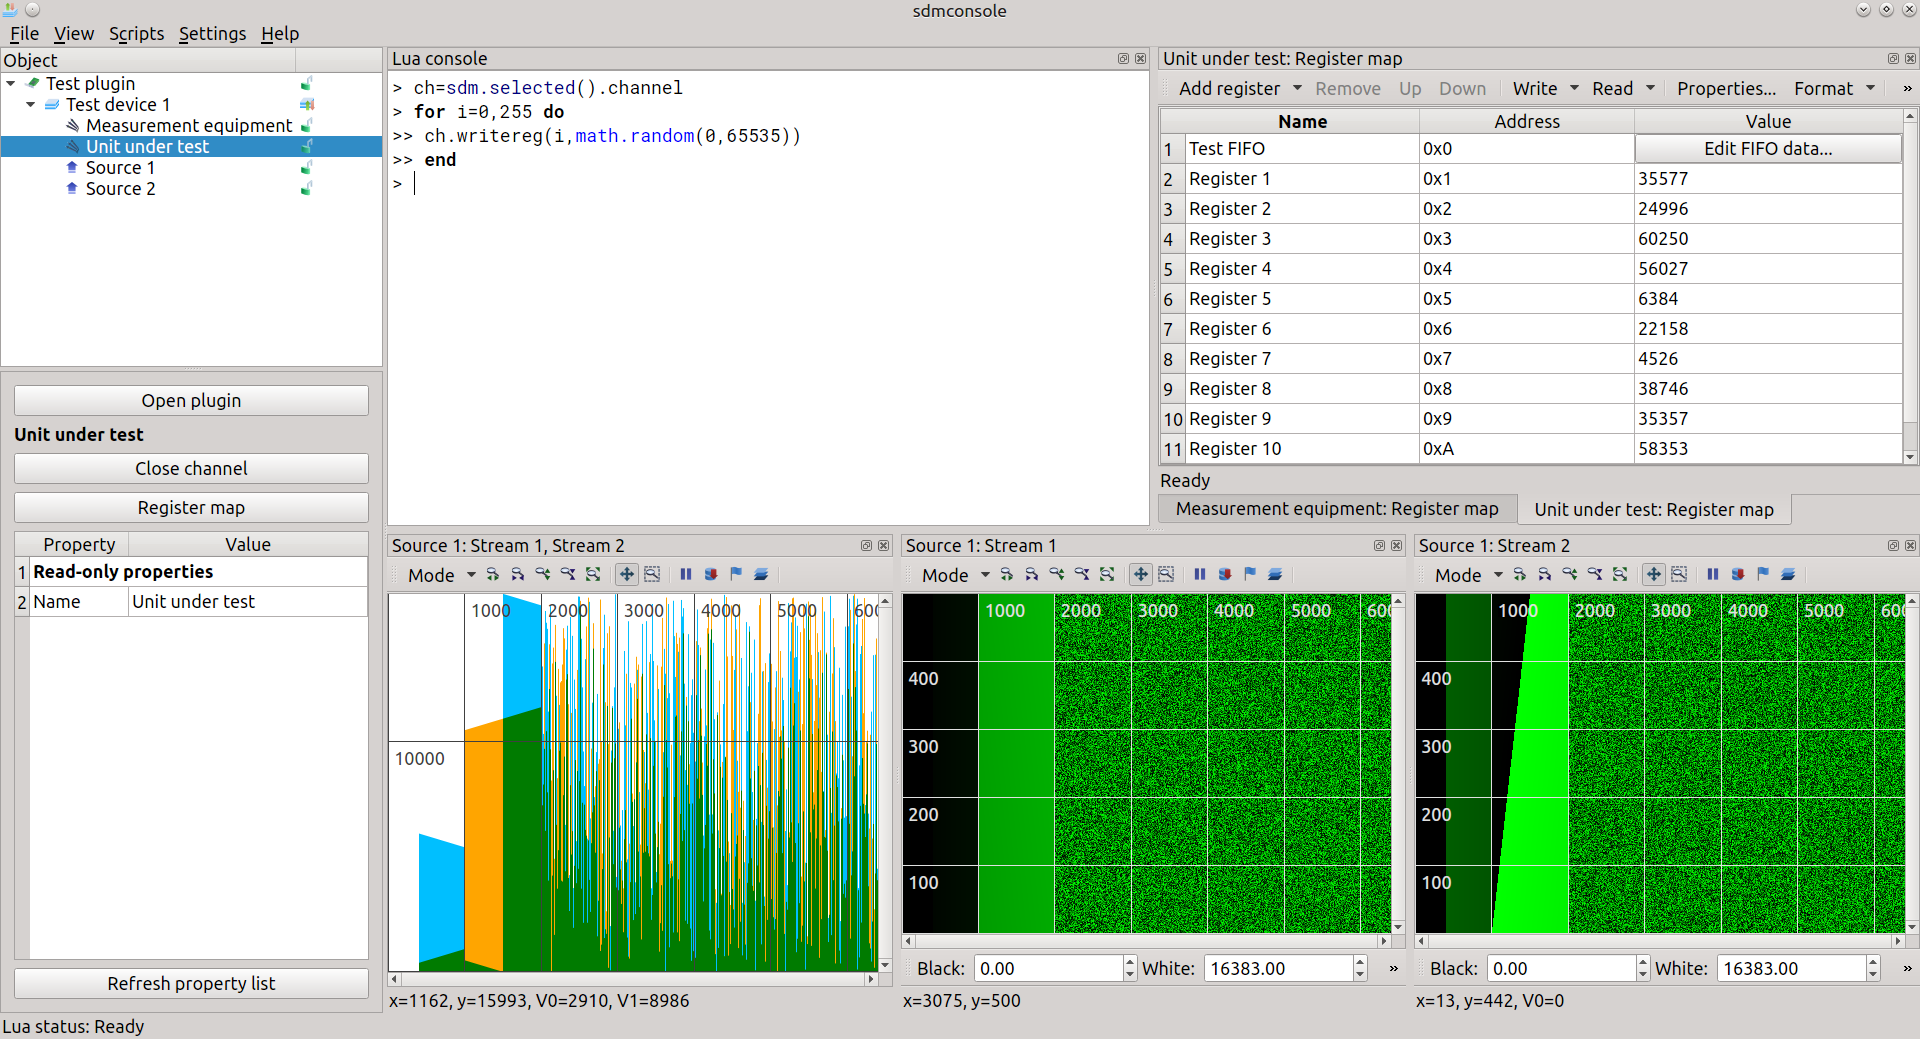
\includegraphics[scale=0.35]{images/sdmconsolemain.png}
\caption{\shellcmd{sdmconsole} main window}
\label{fig:sdmconsolemain}
\end{figure}

The upper part of the sidebar displays the object tree. The lower part contains a set of controls to manage the currently selected object and view or edit its properties.

The dock area is able to contain an arbitrary number of secondary windows. Secondary windows in the dock area can be freely resized and moved by the user. They can also be undocked (detached from the dock area) and docked again. Undocked windows are floating on the desktop as any other top-level window. The \uielement{View} menu provides options to control how new secondary windows are added to the dock area.

On the program startup, the dock area has only one window: the \emph{Lua console} used to execute Lua scripting commands. When closed, the Lua console is not destroyed, just hidden; it can be restored using the \uielement{View} menu.

\section{Basic device management}

Operations with object tree items are performed using controls in the lower part of the sidebar or context menus activated by right-clicking the object tree. Plugins are loaded with the \uielement{Open plugin} sidebar button, the respective context menu item, or the \uielement{File} $\rightarrow$ \uielement{Open plugin\ldots} main menu item. Invoking this command produces a dialog window where the user can select a plugin and a device to load. Alternatively, the device can be opened later, by selecting the plugin in the object tree and clicking on the \uielement{Open device} button. Generally, SDM allows the user to open the same device multiple times (unless prevented by a plugin), which can be useful if several devices are connected to the same workstation.

Selecting a device in the object tree produces a device panel which can be used to connect to the device as well as to open channels and sources. Clicking on the \uielement{Connect} button produces a connection dialog which allows the user to enter connection parameters (a set of parameters is specified by the plugin). These commands are also available from the device's context menu.

An object can be closed by selecting it in the object tree and clicking on a respective panel button. Closing the object also closes all of its children.

\section{Accessing the device's address space}

\shellcmd{sdmconsole} provides a \uielement{Register map} window which is used to access the device's address space. To open this window, select a channel in the object tree and click on the \uielement{Register map} button on the channel panel.

A register map is organized as a set of pages, each of pages being a three-column table. The first column contains an optional name of the register or memory block, the second -- its address, the last column holds the register value or a button to access the memory block data. Using toolbar commands, one can add new pages, section headers, registers and memory blocks. Registers and memory blocks can be written and read by using toolbar buttons or F2 and F3 keys respectively.

By default, the user enters register data directly as a numerical value. Using \uielement{Properties} button, one can replace the text input field in \uielement{Data} column with a drop-down list, a combobox or a push button, to provide a selection of possible values.

Registers and memory blocks can have custom write and/or read actions. A custom action is a Lua script which, if set, is executed on write/read instead of simply writing or reading the register or memory block.

Register map can be saved to a file and loaded from a file.

Detailed description of register map's features is provided in Chapter \ref{ch:registermap}.

\section{Working with data streams}

Data streams are accessed by selecting a source object in the object tree. Clicking on a \uielement{Stream viewer} button opens a dialog where the user can choose one or more streams to view. Streams are displayed by a plotter window which allows the user to select different view modes and provides navigation tools. Plotter window is described in detail in Chapter \ref{ch:plotter}.

A stream or several streams can be also saved to a file by clicking on the \uielement{File writer} button. Files use the MHDB format specified in Appendix \ref{app:mhdbformat}. The MHDB format requires constant packet length that can be entered by the user or detected automatically. Any longer packet will be trimmed, shorter packets will be padded with zeros.

The user can also set the decimation factor which makes SDM deliver only one of each \emph{N} packets. Decimation factor affects both \uielement{Stream viewer} and \uielement{File writer}.

\section{Lua console}

\uielement{Lua console} is used to execute Lua statements interactively. Multi-line blocks are also supported. If a statement returns any values, they are printed in the console window; thus, \expr{\textbf{return} \emph{expression}} statement can be used to display the result of \expr{\emph{expression}} evaluation. For tables, each key/value pair is printed separately; \luaexpr{return _G} prints the global environment.

Table \ref{tab:consolecommands} lists special commands that are executed by the console itself and not passed to the Lua interpreter.

\begin{table}[htbp]
	\caption{Special Lua console commands}
	\label{tab:consolecommands}
	\begin{tabularx}{\textwidth}{lL}
		\toprule
		Command & Description \\
		\midrule
		\shellcmd{clear} & Clear the console window \\
		\shellcmd{quit} & Quit the application \\
		\bottomrule
	\end{tabularx}
\end{table}

Lua console maintains a history of entered commands which can be navigated through using up and down arrow keys. Commands starting with a space are not added to the history.

Script files can be executed using the \luaexpr{dofile()} Lua function, or, if Unicode file name support is desired, \luaexpr{codec.dofile()} (see Subsection \ref{subsec:codec}). Script files can also be dropped on the Lua console or selected in the \uielement{Scripts} menu.

See also Chapter \ref{ch:scripting} for detailed description of SDM Lua extensions.

\chapter{Register map window}
\label{ch:registermap}

Register map window is a versatile tool provided by \shellcmd{sdmconsole} allowing the user to work with the device address space. It is organized as a set of table-based pages (Figure \ref{fig:registermap}).

\begin{figure}[htbp]
\centering
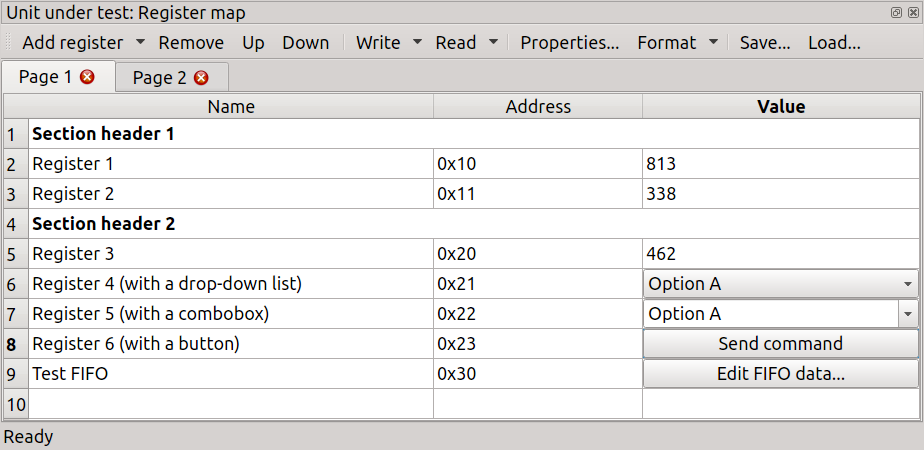
\includegraphics[scale=0.75]{images/registermap.png}
\caption{Register map window}
\label{fig:registermap}
\end{figure}

To add a page, select the \uielement{Add page} menu item which is available after clicking on an arrow near the \uielement{Add register} toolbar button. To change page name, double-click on its tab. To remove page, click on the \uielement{Close} icon on the tab.

Table rows can be of multiple types:

\begin{itemize}
	\item \uielement{Register} (default) normally represents a single value that can be written or read. A register is usually defined by its address (second column), its value is stored in the third column.
	\item \uielement{FIFO} represents a memory block that is mapped to a single register address (contained in the second column). The third column shows a button which can be used to access memory contents and other options.
	\item \uielement{Memory} represents a memory block that occupies a contiguous address range (starting from the address contained in the second column). As above, memory contents can be accessed using a button in the third column.
	\item \uielement{Section} is just a header. It contains only one cell and can't be written or read.
\end{itemize}

Rows can be added, removed and moved using respective toolbar buttons. For \uielement{Register}, \uielement{FIFO} and \uielement{Memory} type rows, the \uielement{Properties} button opens a dialog with additional settings for this row.

Rows of \uielement{Register}, \uielement{FIFO} and \uielement{Memory} types can be written and read using \uielement{Write} and \uielement{Read} toolbar buttons or \uielement{F2} and \uielement{F3} keys respectively. By default, only the selected row is written/read. \uielement{Write} and \uielement{Read} buttons also have menus that can be used to write/read the whole page (or all pages). There is also an option to write automatically when the register data are changed.

SDM represents register addresses and values as unsigned 32-bit integers (see Section \ref{sec:abi}), though register map can also display them as signed if needed. With the \uielement{Format} toolbar button the user can choose number representation for address and data columns (\uielement{As is}, \uielement{Unsigned}, \uielement{Signed} or \uielement{Hexadecimal}). Values entered by the user will be automatically converted to the selected representation (unless the \uielement{As is} option is selected).

\uielement{Save} and \uielement{Load} toolbar buttons are used to save register map contents to a file and load it from a file. All the columns are saved, as well as additional register, FIFO and memory settings.

\section[Register type row]{\uielement{Register} type row}

To add a new row of \uielement{Register} type, click on the \uielement{Add register} toolbar button. For convenience, each page also has an empty row of \uielement{Register} type at the bottom.

By default, the third (data) column contains a text input field where the user can enter a value to write and which displays the value that has been read. By clicking on the \uielement{Properties} toolbar button, one can replace this input field by a drop-down list, a combobox or a push button (Figure \ref{fig:registermapreg}).

\begin{figure}[htbp]
\centering
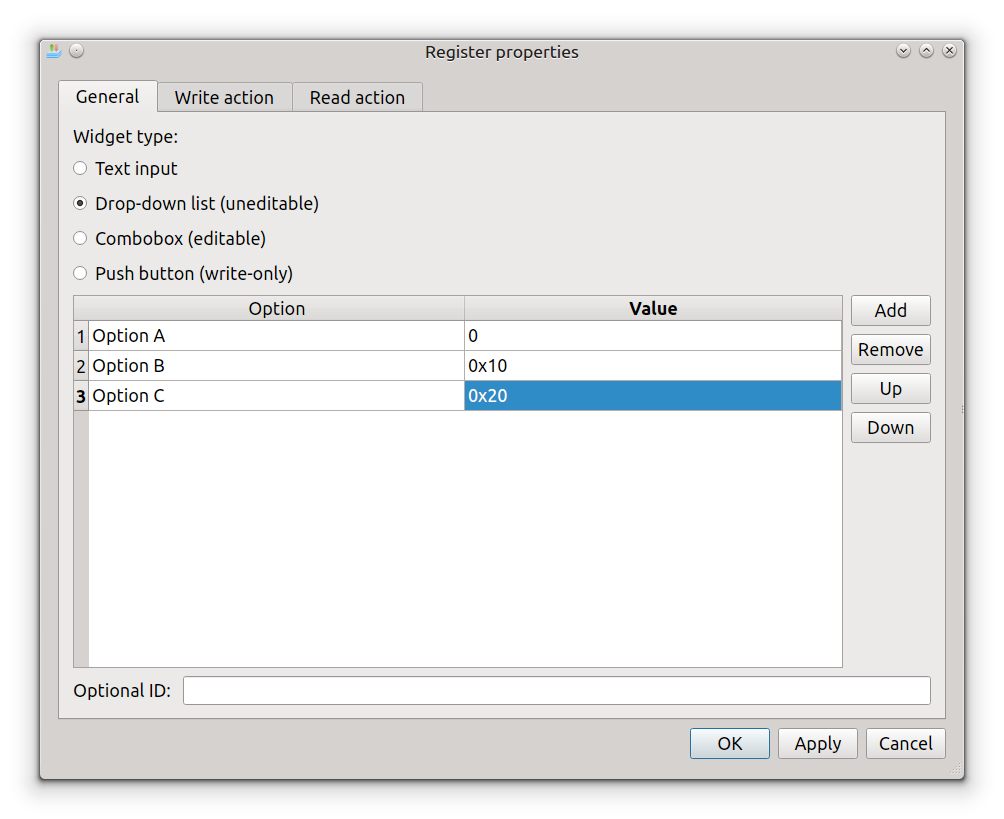
\includegraphics[scale=0.7]{images/registermapreg.png}
\caption{\uielement{Properties} dialog for \uielement{Register} type rows}
\label{fig:registermapreg}
\end{figure}

These input widgets operate as follows:

\begin{itemize}
	\item A drop-down list allows the user to select an option by name. The value that will be written for this option is specified in the \uielement{Properties} dialog. When reading, it will select the option corresponding to the value that has been read. If there is no such option, drop-down list will be converted to a combobox.
	\item A combobox is similar to a drop-down list, but also allows the user to enter a value directly, bypassing suggested options.
	\item A push button is used to write a single value that is specified in the \uielement{Properties} dialog. Push buttons don't display read values at all.
\end{itemize}

The user can also define custom actions that are executed when the register is written and/or read instead of default write/read logic (Section \ref{sec:customactions}).

\section[FIFO and Memory type rows]{\uielement{FIFO} and \uielement{Memory} type rows}

To add a \uielement{FIFO} or \uielement{Memory} type row, select an \uielement{Add FIFO} or \uielement{Add memory} item of the menu attached to the \uielement{Add register} toolbar button.

FIFO and Memory type rows work in a similar way, the difference between them is that FIFO represents a memory block mapped to a single register address, whereas memory block occupies a contiguous range of register addresses.

Like registers, FIFO and memory blocks can have names and addresses. The third column always contains a button that displays \uielement{Properties} dialog for this FIFO or memory (Figure \ref{fig:registermapfifo}).

\begin{figure}[htbp]
\centering
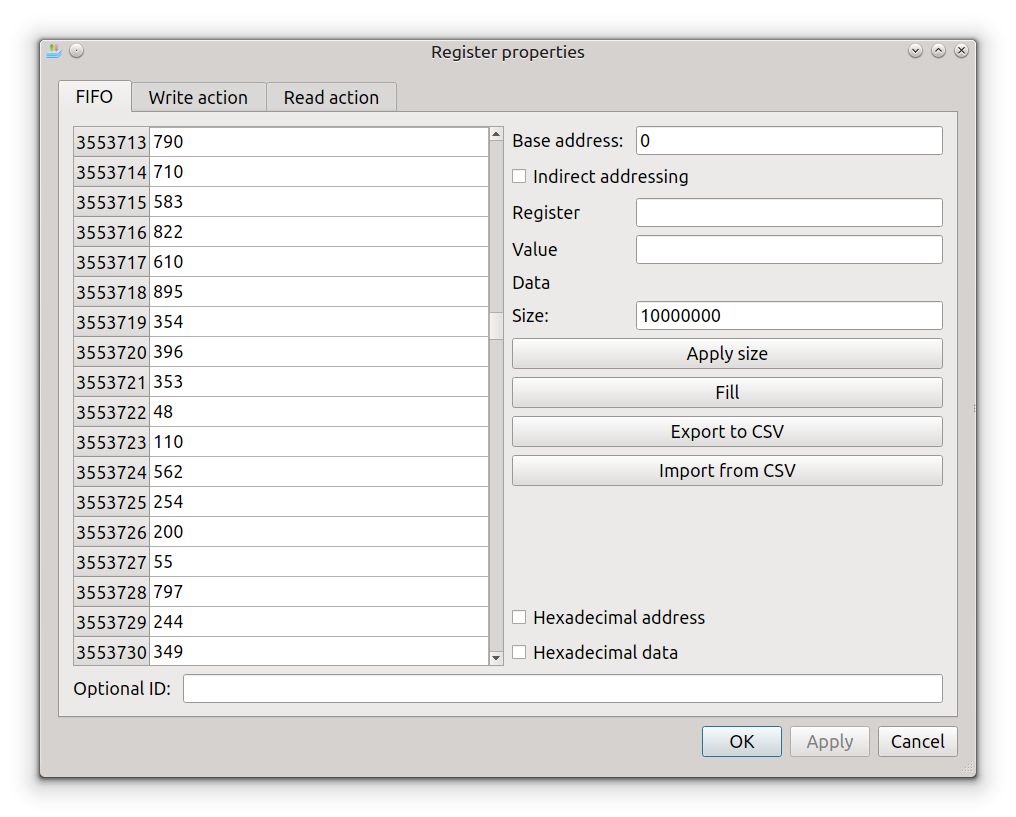
\includegraphics[scale=0.7]{images/registermapfifo.png}
\caption{\uielement{Properties} dialog for \uielement{FIFO} type rows}
\label{fig:registermapfifo}
\end{figure}

\uielement{Base address} field contains the same value as the second table column. \uielement{Indirect addressing} is an optional feature that writes a specified value to the specified register before writing or reading the FIFO or memory.

Data can be exported to a CSV file and imported from a CSV file. Import algorithm is tolerant: it allows any non-digit character or a group of characters to be used as a separator (it doesn't have to be comma, the number of columns also doesn't matter).

Double click on a row number provides a way to scroll the viewport contents to the specified address.

Like registers, FIFO and memory blocks support custom actions (Section \ref{sec:customactions}).

\section{Custom actions}
\label{sec:customactions}

A custom action is a Lua script that is executed whenever the register, FIFO or memory is written and/or read. Custom actions are executed instead of default read/write logic. Write and read actions are separate. Custom actions are set in the \uielement{Properties} dialog (Figure \ref{fig:registermapaction}).

\begin{figure}[htbp]
\centering
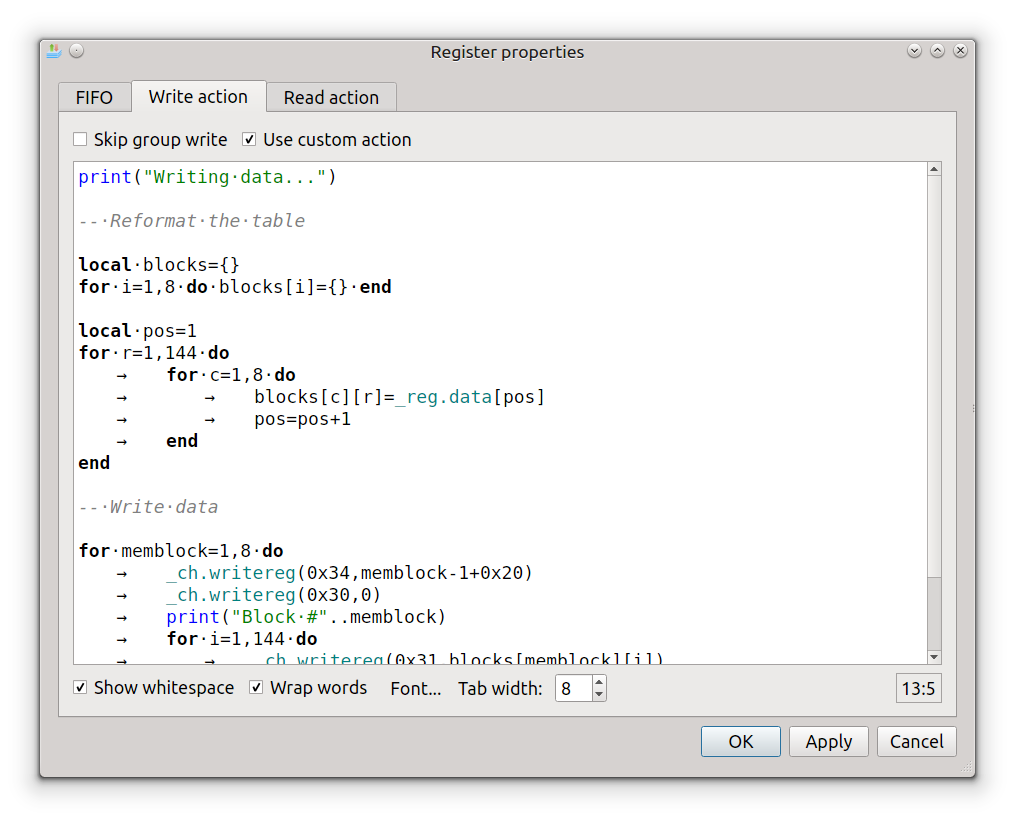
\includegraphics[scale=0.7]{images/registermapaction.png}
\caption{Custom write action}
\label{fig:registermapaction}
\end{figure}

When a custom action is triggered, register map executes the attached Lua script. The script is executed as a Lua chunk in the same environment as all the other scripts (including Lua console commands). In addition, the following variables are made available to the custom action handler:

\begin{itemize}
	\item \luaexpr{_ch} (\objtype{Channel} type object): the channel connected with this register map (Subsection \ref{subsec:luachannel});
	\item \luaexpr{_map} (\objtype{RegisterMap} type object): this register map (Section \ref{sec:luaregistermap});
	\item \luaexpr{_page} (\luatype{integer}): page number;
	\item \luaexpr{_row} (\luatype{integer}): row number;
	\item \luaexpr{_target} (\luatype{string}): \luaexpr{"row"}, \luaexpr{"page"} or \luaexpr{"all"}, depending on what is being written;
	\item \luaexpr{_reg} (\luatype{table}): row data (format is described in Section \ref{sec:luaregistermap}).
\end{itemize}

A write action is not expected to return a value (if it does, the value is ignored). A read action is expected to return the value that is supposed to be displayed (if it doesn't return anything, nothing is changed in the window).

\chapter{Plotter window}
\label{ch:plotter}

Plotter windows are used by \shellcmd{sdmconsole} to display data streams. A plotter window can be displayed by clicking a \uielement{Stream viewer} button on the sidebar after selecting a source in the object tree. One source can have as many plotter windows as needed. Alternatively, plotter window can be created from a Lua script (see Subsection \ref{subsec:luaplotter}).

A plotter window has a top toolbar, a scrollable viewport and an optional bottom toolbar (for some view modes).

Plotter window is merely a representation tool; it doesn't provide means to manage the data source itself.

\section{View modes}

Plotter window supports four view modes: \uielement{Bars} (for bar charts), \uielement{Plot} (for regular line charts), \uielement{Bitmap} (for images), \uielement{Video} (for video data) and \uielement{Binary} (for binary data).

\subsection{\uielement{Bars} and \uielement{Plot} modes}

\uielement{Bars} and \uielement{Plot} modes are used to render bar charts and regular line charts, respectively. Sample numbers, counted from 0, are plotted along the horizontal axis, sample values are plotted along the vertical axis. These modes support multiple layers (Figure \ref{fig:plotterbars}, Figure \ref{fig:plotterplot}). The \uielement{Plot} mode provides a bottom toolbar which allows the user to change the line width and toggle antialiasing on/off.

\begin{figure}[htbp]
\centering
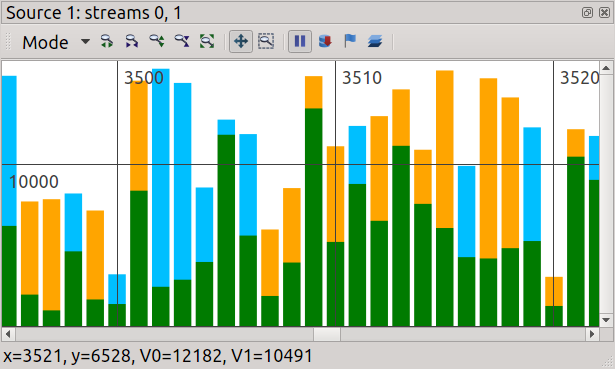
\includegraphics{images/plotterbars.png}
\caption{Plotter window in \uielement{Bars} mode}
\label{fig:plotterbars}
\end{figure}

\begin{figure}[htbp]
\centering
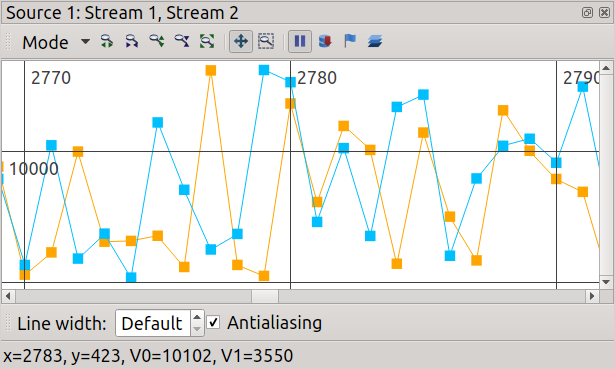
\includegraphics{images/plotterplot.png}
\caption{Plotter window in \uielement{Plot} mode}
\label{fig:plotterplot}
\end{figure}

\subsection{\uielement{Bitmap} mode}

\uielement{Bitmap} mode is used to display multiple lines of graphical data (Figure \ref{fig:plotterbitmap}). Each sample is represented by a pixel. Sample numbers, counted from 0, are plotted along the horizontal axis, packet numbers are plotted along the vertical axis. Sample value is represented by pixel brightness.

In \uielement{Bitmap} mode plotter window can display only one layer.

\begin{figure}[htbp]
\centering
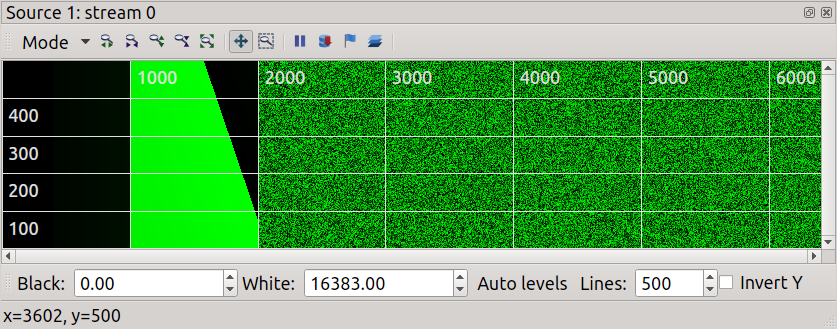
\includegraphics[scale=0.8]{images/plotterbitmap.png}
\caption{Plotter window in \uielement{Bitmap} mode}
\label{fig:plotterbitmap}
\end{figure}

With the bottom toolbar, the user can adjust black and white levels (i.e. mapping between sample values and pixel brightness). If black level is greater than white level, the image is inverted. \uielement{Auto levels} button can be used to detect appropriate levels automatically. Number of displayed lines and a place where new lines are added can also be configured.

\subsection{\uielement{Video} mode}

\uielement{Video} mode is used to display two-dimensional video data (Figure \ref{fig:plottervideo}). Each sample is represented by a pixel. This mode displays only one packet at a time, line width is set by the user. In this mode plotter window can display only one layer.

\begin{figure}[htbp]
\centering
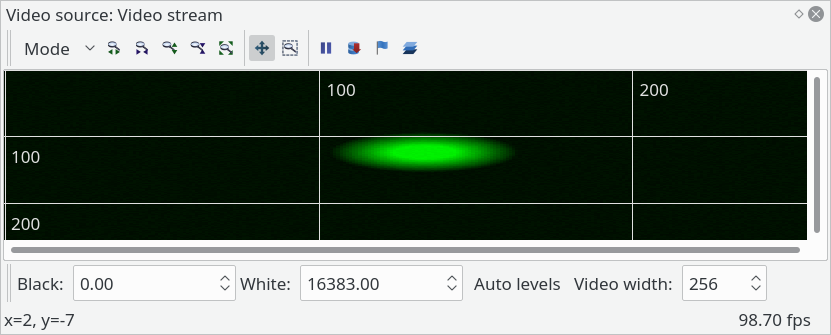
\includegraphics[scale=0.8058]{images/plottervideo.png}
\caption{Plotter window in \uielement{Video} mode}
\label{fig:plottervideo}
\end{figure}

The bottom toolbar can be used to adjust black and white levels (similarly to the \uielement{Bitmap} mode) and configure the line width.

\subsection{\uielement{Binary} mode}

\uielement{Binary} mode is similar to \uielement{Bitmap} mode, the difference being that in \uielement{Binary} mode a pixel represents one bit instead of sample. Number of bits per sample and bit order can be configured (Figure \ref{fig:plotterbinary}).

\begin{figure}[htbp]
\centering
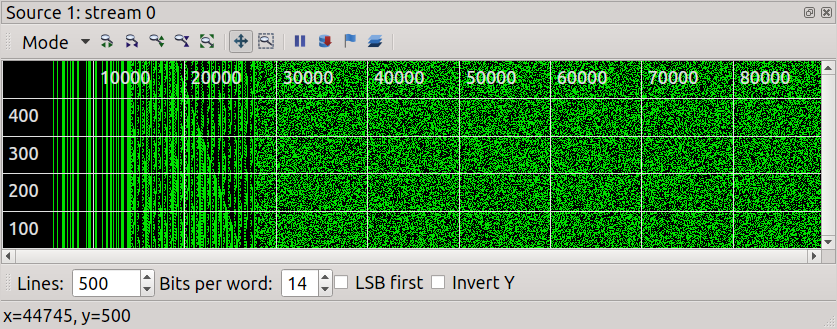
\includegraphics[scale=0.8]{images/plotterbinary.png}
\caption{Plotter window in \uielement{Binary} mode}
\label{fig:plotterbinary}
\end{figure}

\section{Navigation}

Plotter window provides multiple ways to navigate the viewport area, which are summarized in Table \ref{tab:plotternav}. To switch between \uielement{Drag to scroll} and \uielement{Drag to zoom} modes, press right mouse button while in the viewport area, or use the respective toolbar buttons.

\begin{table}[htbp]
\caption{Plotter window navigation}
\label{tab:plotternav}
\begin{tabularx}{\textwidth}{lLL}
\toprule
Control & To scroll & To zoom \\
\toprule
Keyboard & \uielement{Up}, \uielement{Down}, \uielement{Left}, \uielement{Right}, \uielement{PageUp}, \uielement{PageDown} keys & --- \\
\midrule
Wheel & Scroll up/down, with \uielement{Shift}: left/right & With \uielement{Control}: zoom vertically, with \uielement{Shift}+\uielement{Control}: zoom horizontally \\
\midrule
Horizontal wheel & Scroll left/right, with \uielement{Shift}: up/down & With \uielement{Control}: zoom horizontally, with \uielement{Shift}+\uielement{Control}: zoom vertically \\
\midrule
Drag and drop & In \uielement{Drag to scroll} mode & In \uielement{Drag to zoom} mode \\
\midrule
Toolbar & --- & \uielement{Horizontal zoom in}, \uielement{Horizontal zoom out}, \uielement{Vertical zoom in}, \uielement{Vertical zoom out}, \uielement{Fit} \\
\midrule
Double click & --- & Double-click in the viewport area to fit the whole plot (equivalent to the \uielement{Fit} toolbar button) \\
\bottomrule
\end{tabularx}
\end{table}

\section{Managing layers}

Layers representation can be configured with the \uielement{Layers} dialog which can be accessed using the toolbar button (Figure \ref{fig:plotterlayers}). Layer visibility is controlled by a checkbox near the layer name. Colors can be configured on a per-layer basis. Each layer can have a linear transformation applied along the vertical axis; layers are transformed independently of each other. The transformation is based on the following formula:

\begin{displaymath}
y = \mathit{scale} \cdot (x + \mathit{inputOffset}) + \mathit{outputOffset}
\end{displaymath}

\begin{figure}[htbp]
\centering
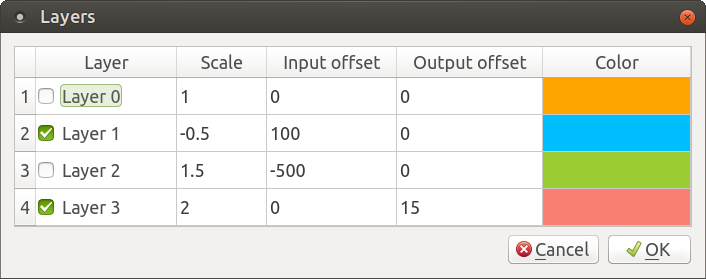
\includegraphics[scale=0.45]{images/plotterlayers.png}
\caption{Layers configuration dialog}
\label{fig:plotterlayers}
\end{figure}

Most of these features are not available for single-layered modes (\uielement{Bitmap}, \uielement{Video} and \uielement{Binary}); in these modes the user can only choose the currently visible layer (making a new layer visible hides the previously visible layer).

\begin{figure}[htbp]
\centering
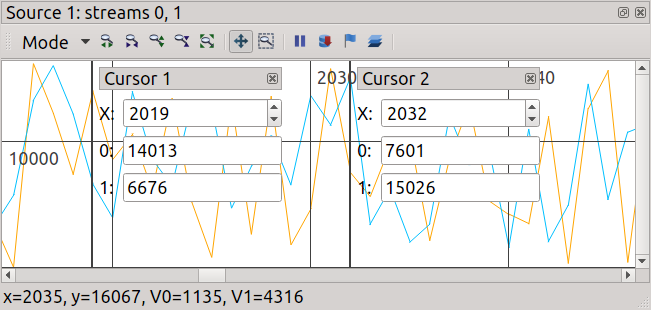
\includegraphics{images/plottercursors.png}
\caption{Cursors}
\label{fig:plottercursors}
\end{figure}

\section{Examining data}

Plotter window status bar displays coordinates and sample values currently hovered by the mouse pointer. The \uielement{Add cursor} toolbar button adds a cursor that shows sample values for a specified horizontal position (Figure \ref{fig:plottercursors}). Any number of cursors can be added; existing cursors can be moved by dragging or by using a spinbox. Both status bar and cursors display original sample values, before any layer transformation is applied. Sample values for hidden layers are not displayed.

\section{Other features}

The \uielement{Freeze} button prevents plot data from updating while allowing the user to navigate the plot as usual. The \uielement{Save image} button exports the contents of the viewport area as an image; both raster (PNG, TIFF, JPEG, BMP) and vector (SVG, PDF) formats are supported. The \uielement{Export data} button exports the currently displayed data in the CSV format.

\chapter{Scripting engine}
\label{ch:scripting}

SDM integrates a scripting engine based on Lua programming language\footnote{\url{https://www.lua.org/}}. The scripting engine uses Lua extension mechanism to provide bindings for the SDM plugin interface as well as (with \shellcmd{sdmconsole}) means to create dialog windows to interact with the user.

The Lua project provides a comprehensive set of documentation which is also shipped with the SDM distribution. The language itself will not be covered in this manual.

Lua extensions provided by the SDM framework are organized as a set of separate libraries, summarized in table \ref{tab:sdmlua}.

\begin{table}[htbp]
	\caption{Core Lua extensions provided by SDM}
	\label{tab:sdmlua}
	\begin{tabularx}{\textwidth}{lL}
		\toprule
		Library & Description \\
		\midrule

		\luaexpr{sdm} & Provides access to SDM plugins, devices, channels and sources \\
		\luaexpr{gui} & Provides means to interact with the user via dialog windows (only for \shellcmd{sdmconsole}) \\
		\luaexpr{codec} & Provides facilities to convert text encoding between UTF-8 (used by SDM) and system encoding \\
		
		\bottomrule
	\end{tabularx}
\end{table}

Libraries provided by the SDM framework are object-oriented. Each library provides a global object with the same name which is used to access the library facilities, including creating other objects. Unlike Lua standard libraries, methods must be invoked with a dot, not a colon (i.e. \luaexpr{channel.writereg()}, not \luaexpr{channel:writereg()}). Each object has an \emph{object type} which is a string stored in its \expr{type} field (not method).

In addition to that, SDM can use Lua extension modules. Modules shipped with the SDM distribution are listed in Table \ref{tab:sdmluaaddons}. More extensions can be added, see Section \ref{sec:luaextensions}. Extension modules are not loaded automatically; to load an extension, use the \luaexpr{require()} Lua function.

\begin{table}[htbp]
	\caption{Addon libraries shipped with SDM}
	\label{tab:sdmluaaddons}
	\begin{tabularx}{\textwidth}{lL}
		\toprule
		Library & Description \\
		\midrule
		
		\luaexpr{luadfic} & Invoke functions from external shared libraries \\
		\luaexpr{luaipsockets} & IP version 4 connectivity \\
		\luaexpr{luart} & Serial port library \\
		
		\bottomrule
	\end{tabularx}
\end{table}

\luaexpr{luadfic}, \luaexpr{luaipsockets} and \luaexpr{luart} are parts of the SDM project, but can be also used with a standalone Lua interpreter.

\section[sdm library]{\expr{sdm} library}

\expr{sdm} library provides access to devices through the SDM plugin interface. Its features are available through the \expr{sdm} global object of \objtype{Bridge} type. A simple example:

\begin{breakshellcmds}\begin{luacode}
-- Open plugin
plugin=sdm.openplugin("testplugin")

-- Open device
device=plugin.opendevice(0)

-- Connect
device.setproperty("IPaddress","127.0.0.1")
device.setproperty("Port","1234")
device.connect()

-- Open channel
channel=device.openchannel(0)

-- Write and read some registers
channel.writereg(0x10,5678)
r=channel.readreg(0x10)
print("Read value: "..r)

-- Open source
source=device.opensource(0)

-- Read stream data
source.selectreadstreams({0,1})
for i=1,10 do
    data0=source.readstream(0,10000)
    print("0: packet of length "..#data0)
    data1=source.readstream(1,10000)
    print("1: packet of length "..#data1)
    source.readnextpacket()
end
\end{luacode}\end{breakshellcmds}

\subsection{\expr{sdm} global object}

%%%%%%%%%%%%%%%%%%%%%%%%%%%%%%
% sdm.openplugin()
%%%%%%%%%%%%%%%%%%%%%%%%%%%%%%

\begin{luafuncprototype}
sdm.openplugin(filename)
\end{luafuncprototype}

\begin{funcdescr}
	Opens a plugin file.
\end{funcdescr}

\begin{funcparams}
	\funcparam{filename} (\luatype{string}): a plugin file name
\end{funcparams}

\begin{funcret}
	Returns a \objtype{Plugin} type object.
\end{funcret}

\begin{funcremarks}
	If \luaexpr{filename} is not an absolute path, it will be resolved relative to the standard SDM plugins directory (Section \ref{sec:installdirectories}). If \luaexpr{filename} has no extension, a platform-specific extension will be appended (\shellcmd{.dll} for Windows, \shellcmd{.so} for Linux).
	
	If a plugin can't be opened for any reason, the function will raise an error.
\end{funcremarks}

%%%%%%%%%%%%%%%%%%%%%%%%%%%%%%
% sdm.plugins()
%%%%%%%%%%%%%%%%%%%%%%%%%%%%%%

\begin{luafuncprototype}
sdm.plugins([index])
\end{luafuncprototype}

\begin{funcdescr}
	Queries the number of opened plugins or gets a \objtype{Plugin} type object corresponding to an opened plugin.
\end{funcdescr}

\begin{funcparams}
	\funcparam{index} (\luatype{integer}, optional): index of an opened plugin (counted from 1)
\end{funcparams}

\begin{funcret}
	When called without parameters, returns the number of opened plugins. When called with an \luaexpr{index} parameter, returns a \objtype{Plugin} type object corresponding to an opened plugin with this index.
\end{funcret}

%%%%%%%%%%%%%%%%%%%%%%%%%%%%%%
% sdm.findobject()
%%%%%%%%%%%%%%%%%%%%%%%%%%%%%%

\begin{luafuncprototype}
sdm.findobject(name [, type])
\end{luafuncprototype}

\begin{funcdescr}
	Finds an opened SDM object with the specified name (and type, if present).
\end{funcdescr}

\begin{funcparams}
	\funcparam{name} (\luatype{string}): object name
	\funcparam{type} (\luatype{string}, optional): object type (\luaexpr{"Plugin"}, \luaexpr{"Device"}, \luaexpr{"Channel"} or \luaexpr{"Source"})
\end{funcparams}

\begin{funcret}
	Returns the requested object, or \luaexpr{nil} if it cannot be found.
\end{funcret}

\begin{funcremarks}
	If there are multiple objects with the same name (and type, if present), it is not specified which of them is returned.
\end{funcremarks}

%%%%%%%%%%%%%%%%%%%%%%%%%%%%%%
% sdm.info()
%%%%%%%%%%%%%%%%%%%%%%%%%%%%%%

\begin{luafuncprototype}
sdm.info(key)
\end{luafuncprototype}

\begin{funcdescr}
	Queries SDM framework information.
\end{funcdescr}

\begin{funcparams}
	\funcparam{key} (\luatype{string}): type of information requested
	\begin{itemize}
		\item \luaexpr{"host"} (\luatype{string}): name of the host program (\luaexpr{"sdmconsole"} or \luaexpr{"sdmhost"})
		\item \luaexpr{"version"} (\luatype{string}): SDM framework version (\expr{"\productversion{}"})
		\item \luaexpr{"os"} (\luatype{string}): operating system type (\luaexpr{"windows"} or \luaexpr{"unix"})
		\item \luaexpr{"uilanguages"} (\luatype{table}): list of user interface languages, where each language is represented by a BCP47 language tag\footnote{\url{https://tools.ietf.org/rfc/rfc5646.txt}} (for example, \luaexpr{\{"en-US","ru-RU"\}})
	\end{itemize}
\end{funcparams}

\begin{funcret}
	Returns the requested value.
\end{funcret}

%%%%%%%%%%%%%%%%%%%%%%%%%%%%%%
% sdm.path()
%%%%%%%%%%%%%%%%%%%%%%%%%%%%%%

\begin{luafuncprototype}
	sdm.path(name)
\end{luafuncprototype}

\begin{funcdescr}
	Queries an SDM system path.
\end{funcdescr}

\begin{funcparams}
	\funcparam{name} (\luatype{string}): requested path (see the Remarks section below)
\end{funcparams}

\begin{funcret}
	Returns an absolute path in a UTF-8 encoded form.
\end{funcret}

\begin{funcremarks}
	\luaexpr{name} can be one of the following:
	
	\begin{itemize}
		\item \luaexpr{"currentdir"}: current directory;
		\item \luaexpr{"homedir"}: home directory of the current user;
		\item \luaexpr{"currentscript"}: a path to the currently executed script, or \luaexpr{nil} if it cannot be obtained;
		\item \luaexpr{"currentscriptdir"}: a path to the directory containing the currently executed script, or \luaexpr{nil} if it cannot be obtained;
		\item \luaexpr{"program"}: a path to the host program executable (e.g. \shellcmd{sdmhost} or \shellcmd{sdmconsole});
		\item \luaexpr{"installprefix"}: SDM installation prefix;
		\item \luaexpr{"bindir"}: SDM binaries directory;
		\item \luaexpr{"pluginsdir"}: SDM plugins directory;
		\item \luaexpr{"luamodulesdir"}: SDM native Lua modules directory;
		\item \luaexpr{"luacmodulesdir"}: SDM binary (``C'') Lua modules directory;
		\item \luaexpr{"qtdir"}: Qt plugins directory (only makes sense on Microsoft Windows);
		\item \luaexpr{"docdir"}: SDM documentation directory;
		\item \luaexpr{"translationsdir"}: \shellcmd{sdmconsole} translations directory;
		\item \luaexpr{"scriptsdir"}: SDM scripts directory;
		\item \luaexpr{"datadir"}: SDM plugin data directory.
	\end{itemize}

	All directory names are encoded as UTF-8 strings. In order to access files in these directories, portable scripts should use \luaexpr{codec.open()} instead of \luaexpr{io.open()} since the latter is not Unicode aware. Alternatively, a string can be converted to the local encoding from UTF8 with \luaexpr{codec.utf8tolocal()}, unless the source string contains characters that can't be represented in the local encoding.
\end{funcremarks}

%%%%%%%%%%%%%%%%%%%%%%%%%%%%%%
% sdm.sleep()
%%%%%%%%%%%%%%%%%%%%%%%%%%%%%%

\begin{luafuncprototype}
sdm.sleep(msec)
\end{luafuncprototype}

\begin{funcdescr}
	Puts the Lua interpreter thread to sleep for a specified time.
\end{funcdescr}

\begin{funcparams}
	\funcparam{msec} (\luatype{integer}): time to sleep for, in milliseconds
\end{funcparams}

%%%%%%%%%%%%%%%%%%%%%%%%%%%%%%
% sdm.time()
%%%%%%%%%%%%%%%%%%%%%%%%%%%%%%

\begin{luafuncprototype}
sdm.time()
\end{luafuncprototype}

\begin{funcdescr}
	Queries the current time.
\end{funcdescr}

\begin{funcret}
	Returns the amount of time from the start of the epoch, in milliseconds. The meaning of epoch depends on an implementation. These function can be used to measure time intervals.
\end{funcret}

%%%%%%%%%%%%%%%%%%%%%%%%%%%%%%
% sdm.lock()
%%%%%%%%%%%%%%%%%%%%%%%%%%%%%%

\begin{luafuncprototype}
sdm.lock(action)
\end{luafuncprototype}

\begin{funcdescr}
	Locks or unlocks the SDM plugin interface.
\end{funcdescr}

\begin{funcparams}
	\funcparam{action} (\luatype{boolean}): \luaexpr{true} to lock, \luaexpr{false} to unlock
\end{funcparams}

\begin{funcremarks}
	When the Lua interpreter invokes an SDM function, \shellcmd{sdmconsole} will prevent access to the SDM plugin interface from other threads (including the GUI thread). However, other threads still can call SDM API functions while Lua interpreter is executing some other code. Sometimes it can be undesirable, notably when reading stream data. This function obtains exclusive access to the SDM plugin interface.
	
	\luaexpr{sdm.lock(true)} can be called multiple times. In order to release lock, \luaexpr{sdm.lock(false)} must be called the same number of times. If Lua interpreter finishes while the SDM plugin interface is still locked, it will be unlocked automatically.
	
	\luaexpr{sdm.lock()} is ignored by \shellcmd{sdmhost} since it doesn't use multiple threads.
\end{funcremarks}

%%%%%%%%%%%%%%%%%%%%%%%%%%%%%%
% sdm.selected()
%%%%%%%%%%%%%%%%%%%%%%%%%%%%%%

\begin{luafuncprototype}
sdm.selected()
\end{luafuncprototype}

\begin{funcdescr}
	Gets an item currently selected in the object tree (\shellcmd{sdmconsole} only).
\end{funcdescr}

\begin{funcret}
	Returns a table with the following fields:
	\begin{itemize}
		\item \luaexpr{plugin} (\objtype{Plugin} type object): currently selected plugin
		\item \luaexpr{device} (\objtype{Device} type object): currently selected device
		\item \luaexpr{channel} (\objtype{Channel} type object): currently selected channel
		\item \luaexpr{source} (\objtype{Source} type object): currently selected source
	\end{itemize}
	
	If a child object is selected, its parent object is also returned as a part of the table (e.g. if \emph{Channel} is selected, \emph{Device} and \emph{Plugin} are also returned). If neither object of the certain type nor its children are selected, the corresponding table field is omitted (which can be tested by comparing its value to \luaexpr{nil}).
\end{funcret}

\subsection{Common property interface}
\label{subsec:luaproperties}

\begin{funcdescr}
	\luaexpr{sdm} library provides a common property interface to access properties of \objtype{Plugin}, \objtype{Device}, \objtype{Channel} and \objtype{Source} type objects.
\end{funcdescr}

%%%%%%%%%%%%%%%%%%%%%%%%%%%%%%
% object.getproperty()
%%%%%%%%%%%%%%%%%%%%%%%%%%%%%%

\begin{luafuncprototype}
\emph{object}.getproperty(name [, defaultvalue])
\end{luafuncprototype}

\begin{funcdescr}
	Gets a property value.
\end{funcdescr}

\begin{funcparams}
	\funcparam{name} (\luatype{string}): property name
	\funcparam{defaultvalue} (\luatype{string}, optional): default property value
\end{funcparams}

\begin{funcret}
	If the requested property exists, returns its value. If the requested property doesn't exist, returns \luaexpr{defaultvalue} if it is present, otherwise returns \luaexpr{nil}.
\end{funcret}

%%%%%%%%%%%%%%%%%%%%%%%%%%%%%%
% object.setproperty()
%%%%%%%%%%%%%%%%%%%%%%%%%%%%%%

\begin{luafuncprototype}
\emph{object}.setproperty(name, value)
\end{luafuncprototype}

\begin{funcdescr}
	Sets the value of \luaexpr{name} property to \luaexpr{value}.
\end{funcdescr}

\begin{funcparams}
	\funcparam{name} (\luatype{string}): property name
	\funcparam{value} (\luatype{string}): property value
\end{funcparams}

%%%%%%%%%%%%%%%%%%%%%%%%%%%%%%
% object.listproperties()
%%%%%%%%%%%%%%%%%%%%%%%%%%%%%%

\begin{luafuncprototype}
\emph{object}.listproperties(name)
\end{luafuncprototype}

\begin{funcdescr}
	Gets a property value as a list.
\end{funcdescr}

\begin{funcparams}
	\funcparam{name} (\luatype{string}): property name
\end{funcparams}

\begin{funcret}
	Returns a table containing list elements.
\end{funcret}

\begin{funcremarks}
	Property lists are described in Section \ref{sec:properties}.
\end{funcremarks}

\begin{funcdescr}
	\luaexpr{sdm} library objects also override \luaexpr{__index} and \luaexpr{__newindex} metamethods, allowing the user to access properties as ordinary table fields:
\end{funcdescr}

\begin{shellcmds}\begin{luacode}
-- The following statements are equivalent
str=device.getproperty("IPaddress")
str=device.IPaddress
str=device["IPaddress"]

-- The following statements are also equivalent
device.setproperty("IPaddress","127.0.0.1")
device.IPaddress="127.0.0.1"
device["IPaddress"]="127.0.0.1"
\end{luacode}\end{shellcmds}

\subsection{\objtype{Plugin} type object}

%%%%%%%%%%%%%%%%%%%%%%%%%%%%%%
% plugin.path()
%%%%%%%%%%%%%%%%%%%%%%%%%%%%%%

\begin{luafuncprototype}
\emph{plugin}.path()
\end{luafuncprototype}

\begin{funcdescr}
	Gets the path to the plugin file.
\end{funcdescr}

\begin{funcret}
	Returns a path to the plugin file (absolute, if available).
\end{funcret}

%%%%%%%%%%%%%%%%%%%%%%%%%%%%%%
% plugin.close()
%%%%%%%%%%%%%%%%%%%%%%%%%%%%%%

\begin{luafuncprototype}
\emph{plugin}.close()
\end{luafuncprototype}

\begin{funcdescr}
	Closes the plugin.
\end{funcdescr}

%%%%%%%%%%%%%%%%%%%%%%%%%%%%%%
% plugin.opendevice()
%%%%%%%%%%%%%%%%%%%%%%%%%%%%%%

\begin{luafuncprototype}
\emph{plugin}.opendevice(id)
\end{luafuncprototype}

\begin{funcdescr}
	Opens a device.
\end{funcdescr}

\begin{funcparams}
	\funcparam{id} (\luatype{integer}): device id (counted from \luaexpr{0})
\end{funcparams}

\begin{funcret}
	Returns a \objtype{Device} type object.
\end{funcret}

%%%%%%%%%%%%%%%%%%%%%%%%%%%%%%
% plugin.devices()
%%%%%%%%%%%%%%%%%%%%%%%%%%%%%%

\begin{luafuncprototype}
\emph{plugin}.devices([index])
\end{luafuncprototype}

\begin{funcdescr}
	Queries the number of opened devices for the plugin or gets a \objtype{Device} type object corresponding to an opened device.
\end{funcdescr}

\begin{funcparams}
	\funcparam{index} (\luatype{integer}, optional): index of an opened device (counted from 1)
\end{funcparams}

\begin{funcret}
	When called without parameters, returns the number of opened devices for the plugin. When called with an \luaexpr{index} parameter, returns a \objtype{Device} type object corresponding to an opened plugin with this index.
\end{funcret}

\begin{funcremarks}
	Note that \luaexpr{index} denotes a position of the device in the object tree and is not the same as device id.
\end{funcremarks}

%%%%%%%%%%%%%%%%%%%%%%%%%%%%%%
% Property interface
%%%%%%%%%%%%%%%%%%%%%%%%%%%%%%

\begin{luafuncprototype}
\emph{plugin}.getproperty(name [, defaultvalue])\\
\emph{plugin}.setproperty(name, value)\\
\emph{plugin}.listproperties(name)
\end{luafuncprototype}

\begin{funcdescr}
	See Subsection \ref{subsec:luaproperties}.
\end{funcdescr}

\subsection{\objtype{Device} type object}

%%%%%%%%%%%%%%%%%%%%%%%%%%%%%%
% device.id()
%%%%%%%%%%%%%%%%%%%%%%%%%%%%%%

\begin{luafuncprototype}
\emph{device}.id()
\end{luafuncprototype}

\begin{funcdescr}
	Gets the device id.
\end{funcdescr}

\begin{funcret}
	Returns the id of the device.
\end{funcret}

%%%%%%%%%%%%%%%%%%%%%%%%%%%%%%
% device.close()
%%%%%%%%%%%%%%%%%%%%%%%%%%%%%%

\begin{luafuncprototype}
\emph{device}.close()
\end{luafuncprototype}

\begin{funcdescr}
	Closes the device.
\end{funcdescr}

%%%%%%%%%%%%%%%%%%%%%%%%%%%%%%
% device.connect()
%%%%%%%%%%%%%%%%%%%%%%%%%%%%%%

\begin{luafuncprototype}
\emph{device}.connect()
\end{luafuncprototype}

\begin{funcdescr}
	Connects to the device.
\end{funcdescr}

\begin{funcremarks}
	If the device requires connection parameters, they are set using the property interface (see Subsection \ref{subsec:luaproperties}).
\end{funcremarks}

%%%%%%%%%%%%%%%%%%%%%%%%%%%%%%
% device.disconnect()
%%%%%%%%%%%%%%%%%%%%%%%%%%%%%%

\begin{luafuncprototype}
\emph{device}.disconnect()
\end{luafuncprototype}

\begin{funcdescr}
	Disconnects from the device.
\end{funcdescr}

%%%%%%%%%%%%%%%%%%%%%%%%%%%%%%
% device.isconnected()
%%%%%%%%%%%%%%%%%%%%%%%%%%%%%%

\begin{luafuncprototype}
\emph{device}.isconnected()
\end{luafuncprototype}

\begin{funcdescr}
	Queries the device connection status.
\end{funcdescr}

\begin{funcret}
	Returns \luaexpr{true} for an active connection, \luaexpr{false} otherwise.
\end{funcret}

%%%%%%%%%%%%%%%%%%%%%%%%%%%%%%
% device.openchannel()
%%%%%%%%%%%%%%%%%%%%%%%%%%%%%%

\begin{luafuncprototype}
\emph{device}.openchannel(id)
\end{luafuncprototype}

\begin{funcdescr}
	Opens a channel.
\end{funcdescr}

\begin{funcparams}
	\funcparam{id} (\luatype{integer}): channel id
\end{funcparams}

\begin{funcret}
	Returns a \objtype{Channel} type object.
\end{funcret}

%%%%%%%%%%%%%%%%%%%%%%%%%%%%%%
% device.channels()
%%%%%%%%%%%%%%%%%%%%%%%%%%%%%%

\begin{luafuncprototype}
\emph{device}.channels([index])
\end{luafuncprototype}

\begin{funcdescr}
	Queries the number of opened channels for the device or gets a \objtype{Channel} type object corresponding to an opened channel.
\end{funcdescr}

\begin{funcparams}
	\funcparam{index} (\luatype{integer}, optional): index of an opened channel (counted from 1)
\end{funcparams}

\begin{funcret}
	When called without parameters, returns the number of opened channels for the device. When called with an \luaexpr{index} parameter, returns a \objtype{Channel} type object corresponding to an opened channel with this index.
\end{funcret}

\begin{funcremarks}
	Note that \luaexpr{index} denotes a position of the channel in the object tree and is not the same as channel id.
\end{funcremarks}

%%%%%%%%%%%%%%%%%%%%%%%%%%%%%%
% device.opensource()
%%%%%%%%%%%%%%%%%%%%%%%%%%%%%%

\begin{luafuncprototype}
\emph{device}.opensource(id)
\end{luafuncprototype}

\begin{funcdescr}
	Opens a source.
\end{funcdescr}

\begin{funcparams}
	\funcparam{id} (\luatype{integer}): source id
\end{funcparams}

\begin{funcret}
	Returns a \objtype{Source} type object.
\end{funcret}

%%%%%%%%%%%%%%%%%%%%%%%%%%%%%%
% device.sources()
%%%%%%%%%%%%%%%%%%%%%%%%%%%%%%

\begin{luafuncprototype}
\emph{device}.sources([index])
\end{luafuncprototype}

\begin{funcdescr}
	Queries the number of opened sources for the device or gets a \objtype{Source} type object corresponding to an opened source.
\end{funcdescr}

\begin{funcparams}
	\funcparam{index} (\luatype{integer}, optional): index of an opened source (counted from 1)
\end{funcparams}

\begin{funcret}
	When called without parameters, returns the number of opened sources for the device. When called with an \luaexpr{index} parameter, returns a \objtype{Source} type object corresponding to an opened source with this index.
\end{funcret}

\begin{funcremarks}
	Note that \luaexpr{index} denotes a position of the source in the object tree and is not the same as source id.
\end{funcremarks}

%%%%%%%%%%%%%%%%%%%%%%%%%%%%%%
% Property interface
%%%%%%%%%%%%%%%%%%%%%%%%%%%%%%

\begin{luafuncprototype}
\emph{device}.getproperty(name [, defaultvalue])\\
\emph{device}.setproperty(name, value)\\
\emph{device}.listproperties(name)
\end{luafuncprototype}

\begin{funcdescr}
	See Subsection \ref{subsec:luaproperties}.
\end{funcdescr}

\subsection{\objtype{Channel} type object}
\label{subsec:luachannel}

%%%%%%%%%%%%%%%%%%%%%%%%%%%%%%
% channel.id()
%%%%%%%%%%%%%%%%%%%%%%%%%%%%%%

\begin{luafuncprototype}
\emph{channel}.id()
\end{luafuncprototype}

\begin{funcdescr}
	Gets the channel id.
\end{funcdescr}

\begin{funcret}
	Returns the id of the channel.
\end{funcret}

%%%%%%%%%%%%%%%%%%%%%%%%%%%%%%
% channel.close()
%%%%%%%%%%%%%%%%%%%%%%%%%%%%%%

\begin{luafuncprototype}
\emph{channel}.close()
\end{luafuncprototype}

\begin{funcdescr}
	Closes the channel.
\end{funcdescr}

%%%%%%%%%%%%%%%%%%%%%%%%%%%%%%
% channel.writereg()
%%%%%%%%%%%%%%%%%%%%%%%%%%%%%%

\begin{luafuncprototype}
\emph{channel}.writereg(addr, value)
\end{luafuncprototype}

\begin{funcdescr}
	Writes to a register.
\end{funcdescr}

\begin{funcparams}
	\funcparam{addr} (\luatype{integer}): register address
	\funcparam{value} (\luatype{integer}): value to write
\end{funcparams}

%%%%%%%%%%%%%%%%%%%%%%%%%%%%%%
% channel.readreg()
%%%%%%%%%%%%%%%%%%%%%%%%%%%%%%

\begin{luafuncprototype}
\emph{channel}.readreg(addr)
\end{luafuncprototype}

\begin{funcdescr}
	Reads from a register.
\end{funcdescr}

\begin{funcparams}
	\funcparam{addr} (\luatype{integer}): register address
\end{funcparams}

\begin{funcret}
	Returns a value read from the register.
\end{funcret}

%%%%%%%%%%%%%%%%%%%%%%%%%%%%%%
% channel.writefifo()
%%%%%%%%%%%%%%%%%%%%%%%%%%%%%%

\begin{luafuncprototype}
\emph{channel}.writefifo(addr, data)
\end{luafuncprototype}

\begin{funcdescr}
	Writes \luaexpr{data} to the FIFO with address \luaexpr{addr}.
\end{funcdescr}

\begin{funcparams}
	\funcparam{addr} (\luatype{integer}): register address
	\funcparam{data} (\luatype{table}): data to write (table of integers)
\end{funcparams}

\begin{funcremarks}
	FIFO represents a memory block mapped to a single register address. Calling \luaexpr{writefifo()} can be more efficient than calling \luaexpr{writereg()} multiple times depending on how the plugin is implemented.
\end{funcremarks}

%%%%%%%%%%%%%%%%%%%%%%%%%%%%%%
% channel.readfifo()
%%%%%%%%%%%%%%%%%%%%%%%%%%%%%%

\begin{luafuncprototype}
\emph{channel}.readfifo(addr, n)
\end{luafuncprototype}

\begin{funcdescr}
	Reads \luaexpr{n} words from the FIFO with address \luaexpr{addr}.
\end{funcdescr}

\begin{funcparams}
	\funcparam{addr} (\luatype{integer}): register address
	\funcparam{n} (\luatype{integer}): number of words to read
\end{funcparams}

\begin{funcremarks}
	FIFO represents a memory block mapped to a single register address. Calling \luaexpr{readfifo()} can be more efficient than calling \luaexpr{readreg()} multiple times depending on how the plugin is implemented.
\end{funcremarks}

%%%%%%%%%%%%%%%%%%%%%%%%%%%%%%
% channel.writemem()
%%%%%%%%%%%%%%%%%%%%%%%%%%%%%%

\begin{luafuncprototype}
\emph{channel}.writemem(addr, data)
\end{luafuncprototype}

\begin{funcdescr}
	Writes \luaexpr{data} to a memory block starting at \luaexpr{addr}.
\end{funcdescr}

\begin{funcparams}
	\funcparam{addr} (\luatype{integer}): register address
	\funcparam{data} (\luatype{table}): data to write
\end{funcparams}

\begin{funcremarks}
	A memory block is a block of consecutive registers. Calling \luaexpr{writemem()} can be more efficient than calling \luaexpr{writereg()} multiple times depending on how the plugin is implemented.
\end{funcremarks}

%%%%%%%%%%%%%%%%%%%%%%%%%%%%%%
% channel.readmem()
%%%%%%%%%%%%%%%%%%%%%%%%%%%%%%

\begin{luafuncprototype}
\emph{channel}.readmem(addr, n)
\end{luafuncprototype}

\begin{funcdescr}
	Reads \luaexpr{n} words from a memory block starting at \luaexpr{addr}.
\end{funcdescr}

\begin{funcparams}
	\funcparam{addr} (\luatype{integer}): register address
	\funcparam{n} (\luatype{integer}): number of words to read
\end{funcparams}

\begin{funcret}
	Returns a \luatype{table} read from the requested address.
\end{funcret}

\begin{funcremarks}
	A memory block is a block of consecutive registers. Calling \luaexpr{readmem()} can be more efficient than calling \luaexpr{readreg()} multiple times depending on how the plugin is implemented.
\end{funcremarks}

%%%%%%%%%%%%%%%%%%%%%%%%%%%%%%
% channel.registermap()
%%%%%%%%%%%%%%%%%%%%%%%%%%%%%%

\begin{luafuncprototype}
\emph{channel}.registermap()
\end{luafuncprototype}

\begin{funcdescr}
	Opens a register map for the channel (\shellcmd{sdmconsole} only).
\end{funcdescr}

\begin{funcret}
	Returns a \objtype{RegisterMap} type object.
\end{funcret}

\begin{funcremarks}
	If a register map windows for this channel is not opened, this function opens it. Otherwise it raises the existing window.
\end{funcremarks}

%%%%%%%%%%%%%%%%%%%%%%%%%%%%%%
% Property interface
%%%%%%%%%%%%%%%%%%%%%%%%%%%%%%

\begin{luafuncprototype}
\emph{channel}.getproperty(name [, defaultvalue])\\
\emph{channel}.setproperty(name, value)\\
\emph{channel}.listproperties(name)
\end{luafuncprototype}

\begin{funcdescr}
	See Subsection \ref{subsec:luaproperties}.
\end{funcdescr}

\subsection{\objtype{Source} type object}

%%%%%%%%%%%%%%%%%%%%%%%%%%%%%%
% source.id()
%%%%%%%%%%%%%%%%%%%%%%%%%%%%%%

\begin{luafuncprototype}
\emph{source}.id()
\end{luafuncprototype}

\begin{funcdescr}
	Gets the source id.
\end{funcdescr}

\begin{funcret}
	Returns the id of the source.
\end{funcret}

%%%%%%%%%%%%%%%%%%%%%%%%%%%%%%
% source.close()
%%%%%%%%%%%%%%%%%%%%%%%%%%%%%%

\begin{luafuncprototype}
\emph{source}.close()
\end{luafuncprototype}

\begin{funcdescr}
	Closes the source.
\end{funcdescr}

%%%%%%%%%%%%%%%%%%%%%%%%%%%%%%
% source.selectreadstreams()
%%%%%%%%%%%%%%%%%%%%%%%%%%%%%%

\begin{luafuncprototype}
\emph{source}.selectreadstreams(streams [, packets [, df]])
\end{luafuncprototype}

\begin{funcdescr}
	Selects data streams to read.
\end{funcdescr}

\begin{funcparams}
	\funcparam{streams} (\luatype{table}): stream ids to select (table of integers)
	\funcparam{packets} (\luatype{integer}, optional): suggested minimum number of packets to deliver consecutively (per stream), the value of \cexpr{0} leaves the decision to the plugin, default value is \cexpr{0}
	\funcparam{df} (\luatype{integer}, optional): suggested decimation factor (a non-binding request to reduce the source bandwidth by the factor of \luaexpr{df}), \cexpr{1} or greater, default value is \cexpr{1}
\end{funcparams}

\begin{funcremarks}
	Note: calling this functions resets the error counter.
	
	See also Section \ref{sec:sourcefunctions} for description of SDM stream semantics.
\end{funcremarks}

%%%%%%%%%%%%%%%%%%%%%%%%%%%%%%
% source.readstream()
%%%%%%%%%%%%%%%%%%%%%%%%%%%%%%

\begin{luafuncprototype}
\emph{source}.readstream(stream, n [, flag])
\end{luafuncprototype}

\begin{funcdescr}
	Reads \luaexpr{n} samples from a stream with id \luaexpr{stream}.
\end{funcdescr}

\begin{funcparams}
	\funcparam{stream} (\luatype{integer}): stream id
	\funcparam{n} (\luatype{integer}): number of samples to read
	\funcparam{flag} (\luatype{string}, optional): one of the following:
		\begin{itemize}
			\item \luaexpr{"all"}: blocking operation, disallow partial read
			\item \luaexpr{"part"}: blocking operation, allow partial read
			\item \luaexpr{"nb"}: non-blocking operation
		\end{itemize}
		
		Default is \luaexpr{"all"}. See also the Remarks below.
\end{funcparams}

\begin{funcret}
	Returns a table of samples read from the stream or empty table at the end of packet. In the non-blocking mode, in addition, returns \luaexpr{nil} if nothing was read because an operation would block.
\end{funcret}

\begin{funcremarks}
	The requested stream must be selected with \luaexpr{selectreadstreams()}.
	
	Data from all streams that were received simultaneously will be delivered also simultaneously. To proceed to the next packet, \luaexpr{readnextpacket()} must be called (see below).
	
	In the blocking mode, if partial read is not allowed, the function returns when (1) the requested number of samples is read, (2) packet ends or (3) an error occurs. If partial read is allowed, in addition, it returns when at least one sample is read and no more data are available for immediate reading. In the non-blocking mode, in addition, the function returns when no data are available for immediate reading.
	
	See also Section \ref{sec:sourcefunctions} for description of SDM stream semantics.
\end{funcremarks}

%%%%%%%%%%%%%%%%%%%%%%%%%%%%%%
% source.readnextpacket()
%%%%%%%%%%%%%%%%%%%%%%%%%%%%%%

\begin{luafuncprototype}
\emph{source}.readnextpacket()
\end{luafuncprototype}

\begin{funcdescr}
	Proceeds to the next packet. This function affects all selected streams.
\end{funcdescr}

%%%%%%%%%%%%%%%%%%%%%%%%%%%%%%
% source.discardpackets()
%%%%%%%%%%%%%%%%%%%%%%%%%%%%%%

\begin{luafuncprototype}
\emph{source}.discardpackets()
\end{luafuncprototype}

\begin{funcdescr}
	Discards data from the receiver buffer. If the stream supports the notion of packets, the next operation will read from the start of the packet.
\end{funcdescr}

\begin{funcremarks}
	Note: calling this functions resets the error counter.
\end{funcremarks}

%%%%%%%%%%%%%%%%%%%%%%%%%%%%%%
% source.readstreamerrors()
%%%%%%%%%%%%%%%%%%%%%%%%%%%%%%

\begin{luafuncprototype}
\emph{source}.readstreamerrors()
\end{luafuncprototype}

\begin{funcret}
	Returns the number of stream errors for the source.
\end{funcret}

\begin{funcremarks}
	Stream error is a condition when consecutive operations read non-consecutive data.
\end{funcremarks}

%%%%%%%%%%%%%%%%%%%%%%%%%%%%%%
% source.addviewer()
%%%%%%%%%%%%%%%%%%%%%%%%%%%%%%

\begin{luafuncprototype}
\emph{source}.addviewer(streams [, mode [, multilayer]])
\end{luafuncprototype}

\begin{funcdescr}
	Opens a plotter window to display stream data for the source (\shellcmd{sdmconsole} only).
\end{funcdescr}

\begin{funcparams}
	\funcparam{streams} (\luatype{table}): a set of stream ids to display
	\funcparam{mode} (\luatype{string}): viewer mode: \luaexpr{"bars"}, \luaexpr{"plot"}, \luaexpr{"bitmap"}, \luaexpr{"video"} or \luaexpr{"binary"}
	\funcparam{multilayer} (\luatype{integer}): a non-zero value activates the \uielement{Cycle through layers} option and sets the number of layers to cycle through (ignored if \luaexpr{streams} contains more than 1 element)
\end{funcparams}

%%%%%%%%%%%%%%%%%%%%%%%%%%%%%%
% Property interface
%%%%%%%%%%%%%%%%%%%%%%%%%%%%%%

\begin{luafuncprototype}
\emph{source}.getproperty(name [, defaultvalue])\\
\emph{source}.setproperty(name, value)\\
\emph{source}.listproperties(name)
\end{luafuncprototype}

\begin{funcdescr}
	See Subsection \ref{subsec:luaproperties}.
\end{funcdescr}

\section[gui library]{\expr{gui} library}

\expr{gui} library is an \shellcmd{sdmconsole} Lua extension allowing the script developer to create dialog boxes to interact with the user. It includes simple modal dialogs (such as message boxes) that are created by calling methods of the \expr{gui} global object (of \objtype{DialogServer} type) and destroyed before the method returns, as well as more complex modeless windows that are represented as separate objects.

\subsection{\expr{gui} global object}
\label{subsec:luadialogserver}

%%%%%%%%%%%%%%%%%%%%%%%%%%%%%%
% gui.screen()
%%%%%%%%%%%%%%%%%%%%%%%%%%%%%%

\begin{luafuncprototype}
gui.screen()
\end{luafuncprototype}

\begin{funcdescr}
	Gets the dimensions of the active screen.
\end{funcdescr}

\begin{funcret}
	Returns the application's active screen dimensions in pixels (width and height, as 2 return values).
\end{funcret}

%%%%%%%%%%%%%%%%%%%%%%%%%%%%%%
% gui.messagebox()
%%%%%%%%%%%%%%%%%%%%%%%%%%%%%%

\begin{luafuncprototype}
gui.messagebox(message [, title [, icon [, buttons]]])
\end{luafuncprototype}

\begin{funcdescr}
	Displays a modal message box (Figure \ref{fig:messagebox}).
\end{funcdescr}

\begin{figure}[htbp]
\centering
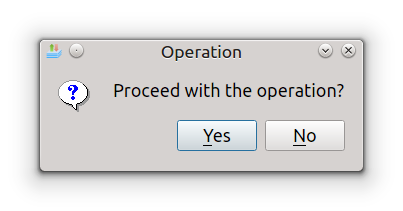
\includegraphics{images/messagebox.png}
\caption{Message box window}
\label{fig:messagebox}
\end{figure}

\begin{funcparams}
	\funcparam{message} (\luatype{string}): a message to display
	\funcparam{title} (\luatype{string}, optional): window title
	\funcparam{icon} (\luatype{string}, optional): icon, one of the following:
	\begin{itemize}
		\item \luaexpr{"error"}
		\item \luaexpr{"warning"}
		\item \luaexpr{"information"}
		\item \luaexpr{"question"}
		\item \luaexpr{""} (no icon)
	\end{itemize}
	\funcparam{buttons} (\luatype{string}, optional): buttons, a comma-separated string containing one or more of the following: \luaexpr{"ok"}, \luaexpr{"cancel"}, \luaexpr{"yes"}, \luaexpr{"no"}; the first button in the string will be selected by default.
\end{funcparams}

\begin{funcret}
	Returns a string corresponding to pressed button.
\end{funcret}

\begin{funcexamples}
\begin{shellcmds}\begin{luacode}
r=gui.messagebox("Proceed with the operation?","Operation","question","yes,no")
if r~="yes" then return end
\end{luacode}\end{shellcmds}
\end{funcexamples}

%%%%%%%%%%%%%%%%%%%%%%%%%%%%%%
% gui.inputdialog()
%%%%%%%%%%%%%%%%%%%%%%%%%%%%%%

\begin{luafuncprototype}
gui.inputdialog(title, label [, value])
\end{luafuncprototype}

\begin{funcdescr}
	Displays a simple modal dialog box allowing the user to enter a string (Figure \ref{fig:inputdialog1}) or select an option from a drop-down list (Figure \ref{fig:inputdialog2}).
\end{funcdescr}

\begin{figure}[htbp]
\centering
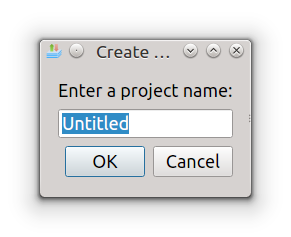
\includegraphics{images/inputdialog1.png}
\caption{Input dialog window (with a text input field)}
\label{fig:inputdialog1}
\end{figure}

\begin{figure}[htbp]
\centering
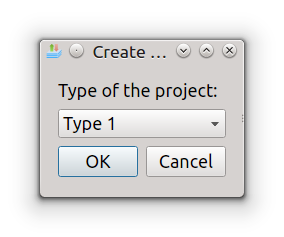
\includegraphics{images/inputdialog2.png}
\caption{Input dialog window (with a drop-down list)}
\label{fig:inputdialog2}
\end{figure}

\begin{funcparams}
	\funcparam{title} (\luatype{string}): window title
	\funcparam{label} (\luatype{string}): label (text that is displayed in the input dialog box)
	\funcparam{value} (\luatype{string} or \luatype{table}, optional): a string containing initial value of the text input field, or a table consisting of strings to populate the drop-down list
\end{funcparams}

\begin{funcret}
	Returns a string entered by the user or selected from the drop-down list, or \luaexpr{nil} if \uielement{Cancel} button was pressed.
\end{funcret}

\begin{funcremarks}
	When \luaexpr{value} is not present, the user is asked to enter a string in a text input field. When \luaexpr{value} is of \luatype{string} type, the field is initialized with the provided string. When \luaexpr{value} is of \luatype{table} type, the text input field is replaced with a drop-down list containing strings from the table.
	
	For more complex input, consider using a \objtype{FormDialog} type object (Subsection \ref{subsec:formdialog}).
\end{funcremarks}

\begin{funcexamples}
\begin{shellcmds}\begin{luacode}
projectname=gui.inputdialog("Create project","Enter a project name:","Untitled")
projecttype=gui.inputdialog("Create project","Type of the project:",{"Type 1","Type 2"})
\end{luacode}\end{shellcmds}
\end{funcexamples}

%%%%%%%%%%%%%%%%%%%%%%%%%%%%%%
% gui.filedialog()
%%%%%%%%%%%%%%%%%%%%%%%%%%%%%%

\begin{luafuncprototype}
gui.filedialog(mode [, filter])
\end{luafuncprototype}

\begin{funcdescr}
	Displays a standard modal dialog box allowing the user to choose a file or a directory (Figure \ref{fig:filedialog}).
\end{funcdescr}

\begin{figure}[htbp]
\centering
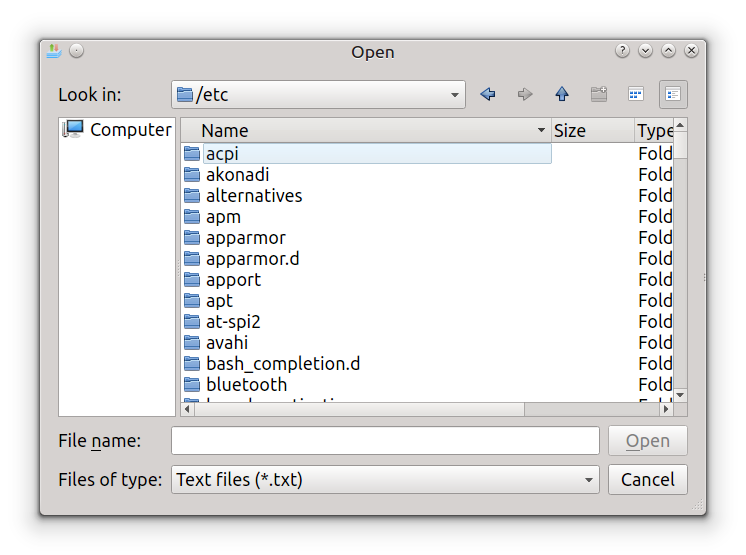
\includegraphics[scale=0.8]{images/filedialog.png}
\caption{File dialog window}
\label{fig:filedialog}
\end{figure}

\begin{funcparams}
	\funcparam{mode} (\luatype{string}): \luaexpr{"open"}, \luaexpr{"save"} or \luaexpr{"dir"}
	\funcparam{filter} (\luatype{string}, optional): file name filter
\end{funcparams}

\begin{funcret}
	Returns a path to the selected file, or \luaexpr{nil} if \uielement{Cancel} was pressed.
\end{funcret}

\begin{funcremarks}
	A file name filter is a string containing a file name mask and an optional description. Multiple filters can be separated by a double semicolon. For example:
\begin{shellcmds}\begin{luacode}
"*.txt"
"Text files (*.txt)"
"Image files (*.png *.jpg *.gif *.bmp)"
"Text files (*.txt);;All files (*)"
\end{luacode}\end{shellcmds}
	\luaexpr{"*.*"} should not be used as a mask for all files since some files don't have an extension.
\end{funcremarks}

\begin{funcexamples}
\begin{shellcmds}\begin{luacode}
filename=gui.filedialog("open","Text files (*.txt);;All files (*)")
if not filename then return end
\end{luacode}\end{shellcmds}
\end{funcexamples}

%%%%%%%%%%%%%%%%%%%%%%%%%%%%%%
% gui.createdialog()
%%%%%%%%%%%%%%%%%%%%%%%%%%%%%%

\begin{luafuncprototype}
gui.createdialog(dialog [, ...])
\end{luafuncprototype}

\begin{funcdescr}
	Creates a modeless dialog window.
\end{funcdescr}

\begin{funcparams}
	\funcparam{dialog} (\luatype{string}): dialog type, one of the following:
	\begin{itemize}
		\item \luaexpr{"progress"} (a progress bar window)
		\item \luaexpr{"form"} (a table-based form window)
		\item \luaexpr{"textviewer"} (a text viewer window)
		\item \luaexpr{"plotter"} (a plotter window)
	\end{itemize}
	\item Other parameters, if any, are passed to the dialog constructor.
\end{funcparams}

\begin{funcret}
	Returns a dialog object. Type of the object depends on \luaexpr{dialog} argument.
\end{funcret}

\begin{funcremarks}
	The dialog window is hidden after creation; to show it, invoke the \luaexpr{show()} method with \luaexpr{true} as an argument (the plotter window is an exception to this). Similarly, the dialog object is not destroyed when the dialog is closed; this allows the developer to query it for information (e.g. user input). To destroy the dialog object, invoke the \luaexpr{close()} method. Alternatively, the dialog can be destroyed automatically by the owner.
	
	The dialog object's lifecycle is managed by the Lua server. When the object goes out of scope in Lua, it becomes eligible for destruction by the Lua garbage collector. The dialog will also be destroyed when the application main window is closed.
\end{funcremarks}

\subsection{Common modeless dialog interface}
\label{subsec:luamodelessdialog}

\begin{funcdescr}
	\luaexpr{gui} library provides a common interface to manage modeless windows represented by \objtype{ProgressDialog}, \objtype{FormDialog}, \objtype{TextViewer} and \objtype{Plotter} type objects.
\end{funcdescr}

%%%%%%%%%%%%%%%%%%%%%%%%%%%%%%
% dialog.show()
%%%%%%%%%%%%%%%%%%%%%%%%%%%%%%

\begin{luafuncprototype}
\emph{dialog}.show([action])
\end{luafuncprototype}

\begin{funcdescr}
	Queries the window visibility state and optionally shows or hides the window.
\end{funcdescr}

\begin{funcparams}
	\funcparam{action} (\luatype{boolean}, optional): \luaexpr{true} to show, \luaexpr{false} to hide
\end{funcparams}

\begin{funcret}
	Returns previous window visibility state.
\end{funcret}

%%%%%%%%%%%%%%%%%%%%%%%%%%%%%%
% dialog.close()
%%%%%%%%%%%%%%%%%%%%%%%%%%%%%%

\begin{luafuncprototype}
\emph{dialog}.close()
\end{luafuncprototype}

\begin{funcdescr}
	Closes the window and destroys the object, freeing all the resources.
\end{funcdescr}

\begin{funcremarks}
	Attempts to access the dialog's methods after it has been destroyed will result in an error being raised.
\end{funcremarks}

%%%%%%%%%%%%%%%%%%%%%%%%%%%%%%
% dialog.settitle()
%%%%%%%%%%%%%%%%%%%%%%%%%%%%%%

\begin{luafuncprototype}
\emph{dialog}.settitle([title])
\end{luafuncprototype}

\begin{funcdescr}
	Queries the current window title and optionally sets it to a new value.
\end{funcdescr}

\begin{funcparams}
	\funcparam{title} (\luatype{string}, optional): new window title
\end{funcparams}

\begin{funcret}
	Returns previous window title.
\end{funcret}

%%%%%%%%%%%%%%%%%%%%%%%%%%%%%%
% dialog.resize()
%%%%%%%%%%%%%%%%%%%%%%%%%%%%%%

\begin{luafuncprototype}
\emph{dialog}.resize([width, height])
\end{luafuncprototype}

\begin{funcdescr}
	Queries the current window size and optionally resizes the window.
\end{funcdescr}

\begin{funcparams}
	\funcparam{width} (\luatype{integer}, optional): new width
	\funcparam{height} (\luatype{integer}, optional): new height
\end{funcparams}

\begin{funcret}
	Returns previous window width and height as 2 return values.
\end{funcret}

\begin{funcremarks}
	\luaexpr{width} and \luaexpr{height} must be either both present or both absent.
\end{funcremarks}

%%%%%%%%%%%%%%%%%%%%%%%%%%%%%%
% dialog.move()
%%%%%%%%%%%%%%%%%%%%%%%%%%%%%%

\begin{luafuncprototype}
\emph{dialog}.move()\\
\emph{dialog}.move(left, top)\\
\emph{dialog}.move("center")
\end{luafuncprototype}

\begin{funcdescr}
	Queries the current window position and optionally moves the window.
\end{funcdescr}

\begin{funcparams}
	\funcparam{left} (\luatype{integer}, optional): new x coordinate of the top-left corner
	\funcparam{top} (\luatype{integer}, optional): new y coordinate of the top-left corner
	\funcparam{"center"} (\luatype{string}, optional)
\end{funcparams}

\begin{funcret}
	Returns previous coordinates of the top-left corner as 2 return values.
\end{funcret}

\begin{funcremarks}
	When invoked in the first form, queries current top-level corner position. In the second form moves the window to the specified position on the desktop. In the third form centers the window on the desktop.
\end{funcremarks}

\subsection{\objtype{ProgressDialog} type object}

A progress dialog is used to display the status of a long operation. It can be created by the \luaexpr{gui.createdialog()} function. An example is shown on Figure \ref{fig:progressdialog}.

\begin{shellcmds}\begin{luacode}
progress=gui.createdialog("progress","Waiting for completion...",0,10)
progress.setvalue(0)
for i=1,10 do
    sdm.sleep(1000)
    progress.setvalue(i)
    if progress.canceled() then
        progress.close()
        return
    end
end
\end{luacode}\end{shellcmds}

\begin{figure}[htbp]
\centering
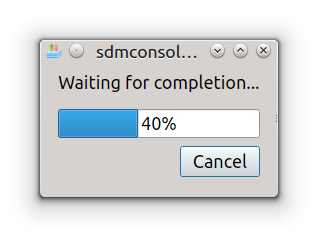
\includegraphics{images/progressdialog.png}
\caption{Progress dialog window}
\label{fig:progressdialog}
\end{figure}

%%%%%%%%%%%%%%%%%%%%%%%%%%%%%%
% Constructor
%%%%%%%%%%%%%%%%%%%%%%%%%%%%%%

\begin{luafuncprototype}
gui.createdialog("progress") \\
gui.createdialog("progress", text) \\
gui.createdialog("progress", text, max) \\
gui.createdialog("progress", text, min, max)
\end{luafuncprototype}

\begin{funcdescr}
	Creates a progress dialog.
\end{funcdescr}

\begin{funcparams}
	\funcparam{text} (\luatype{string}, optional): text displayed in the dialog box
	\funcparam{min} (\luatype{integer}, optional): minimum value (\luaexpr{0} if omitted)
	\funcparam{max} (\luatype{integer}, optional): maximum value (\luaexpr{100} if omitted)
\end{funcparams}

\begin{funcret}
	Returns a \objtype{ProgressDialog} type object.
\end{funcret}

%%%%%%%%%%%%%%%%%%%%%%%%%%%%%%
% progress.setvalue()
%%%%%%%%%%%%%%%%%%%%%%%%%%%%%%

\begin{luafuncprototype}
\emph{progress}.setvalue(value)
\end{luafuncprototype}

\begin{funcdescr}
	Sets a progress bar value.
\end{funcdescr}

\begin{funcparams}
	\funcparam{value} (\luatype{integer}): new progress bar value
\end{funcparams}

\begin{funcremarks}
	The value must be in the range specified by the 
	\luaexpr{setrange()} method or the constructor. Invoking \luaexpr{setvalue(0)} shows the dialog automatically; it is not needed to call \luaexpr{show(true)}. Invoking \luaexpr{setvalue()} with a maximum value as an argument hides the dialog.
\end{funcremarks}

%%%%%%%%%%%%%%%%%%%%%%%%%%%%%%
% progress.settext()
%%%%%%%%%%%%%%%%%%%%%%%%%%%%%%

\begin{luafuncprototype}
\emph{progress}.settext(text)
\end{luafuncprototype}

\begin{funcdescr}
	Sets a text string to be displayed in the dialog box.
\end{funcdescr}

\begin{funcparams}
	\funcparam{text} (\luatype{string}): new text string to display
\end{funcparams}

%%%%%%%%%%%%%%%%%%%%%%%%%%%%%%
% progress.setrange()
%%%%%%%%%%%%%%%%%%%%%%%%%%%%%%

\begin{luafuncprototype}
\emph{progress}.setrange(min, max)
\end{luafuncprototype}

\begin{funcdescr}
	Sets the progress bar range.
\end{funcdescr}

\begin{funcparams}
	\funcparam{min} (\luatype{integer}): minimum value
	\funcparam{max} (\luatype{integer}): maximum value
\end{funcparams}

\begin{funcremarks}
	Sometimes the maximum value is not known (i.e. when downloading a file of unknown size). In this case both \luaexpr{min} and \luaexpr{max} should be set to \luaexpr{0}. The dialog must be shown explicitly with \luaexpr{show(true)}; do not call \luaexpr{setvalue(0)} since it will close the dialog.
\end{funcremarks}

%%%%%%%%%%%%%%%%%%%%%%%%%%%%%%
% progress.reset()
%%%%%%%%%%%%%%%%%%%%%%%%%%%%%%

\begin{luafuncprototype}
\emph{progress}.reset()
\end{luafuncprototype}

\begin{funcdescr}
	Resets the progress bar to an initial state and hides the dialog window.
\end{funcdescr}

%%%%%%%%%%%%%%%%%%%%%%%%%%%%%%
% progress.canceled()
%%%%%%%%%%%%%%%%%%%%%%%%%%%%%%

\begin{luafuncprototype}
\emph{progress}.canceled()
\end{luafuncprototype}

\begin{funcdescr}
	Queries whether the \uielement{Cancel} button has been clicked.
\end{funcdescr}

\begin{funcret}
	Returns \luaexpr{true} if the \uielement{Cancel} button has been clicked or \luaexpr{false} otherwise. After the \uielement{Cancel} button has been clicked, this method will return \luaexpr{true} until \luaexpr{reset()} is invoked.
\end{funcret}

%%%%%%%%%%%%%%%%%%%%%%%%%%%%%%
% Common methods
%%%%%%%%%%%%%%%%%%%%%%%%%%%%%%

\begin{luafuncprototype}
\emph{progress}.show([action]) \\
\emph{progress}.close() \\
\emph{progress}.settitle([title]) \\
\emph{progress}.resize([width, height]) \\
\emph{progress}.move(...)
\end{luafuncprototype}

\begin{funcdescr}
	See Subsection \ref{subsec:luamodelessdialog}.
\end{funcdescr}

\subsection{\objtype{FormDialog} type object}
\label{subsec:formdialog}

A form dialog is used to request more complex user input than is possible by using \luaexpr{gui.inputdialog()}. It can be created by the \luaexpr{gui.createdialog()} function. An example is shown on Figure \ref{fig:formdialog}.

\begin{shellcmds}\begin{luacode}
form=gui.createdialog("form","Connection settings:")
form.addtextoption("Host","192.168.1.100")
form.addlistoption("Protocol",{"TCP","UDP"})
form.addfileoption("Picture to send","open","","JPEG Images (*.jpg *.jpeg);;All files (*)")
r=form.exec()
if not r then return end
print("Name is "..form.getoption(1))
print("Gender is "..form.getoption(2))
print("Photo file path is "..form.getoption(3))
\end{luacode}\end{shellcmds}

\begin{figure}[htbp]
\centering
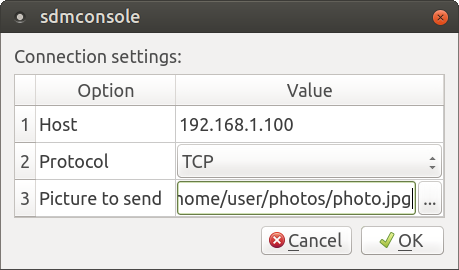
\includegraphics[width=0.8\textwidth]{images/formdialog.png}
\caption{Form dialog window}
\label{fig:formdialog}
\end{figure}

%%%%%%%%%%%%%%%%%%%%%%%%%%%%%%
% Constructor
%%%%%%%%%%%%%%%%%%%%%%%%%%%%%%

\begin{luafuncprototype}
gui.createdialog("form" [, text])
\end{luafuncprototype}

\begin{funcdescr}
	Creates a form dialog.
\end{funcdescr}

\begin{funcparams}
	\funcparam{text} (\luatype{string}, optional): text displayed in the dialog box
\end{funcparams}

\begin{funcret}
	Returns a \objtype{FormDialog} type object.
\end{funcret}

%%%%%%%%%%%%%%%%%%%%%%%%%%%%%%
% form.settext()
%%%%%%%%%%%%%%%%%%%%%%%%%%%%%%

\begin{luafuncprototype}
\emph{form}.settext([text])
\end{luafuncprototype}

\begin{funcdescr}
	Queries the current text string displayed in the dialog box and optionally sets it to the new value.
\end{funcdescr}

\begin{funcparams}
	\funcparam{text} (\luatype{string}, optional): new text string to display
\end{funcparams}

\begin{funcret}
	Returns a previous dialog text string.
\end{funcret}

%%%%%%%%%%%%%%%%%%%%%%%%%%%%%%
% form.addtextoption()
%%%%%%%%%%%%%%%%%%%%%%%%%%%%%%

\begin{luafuncprototype}
\emph{form}.addtextoption(name [, value])
\end{luafuncprototype}

\begin{funcdescr}
	Adds a new text input field to the form.
\end{funcdescr}

\begin{funcparams}
	\funcparam{name} (\luatype{string}): option name
	\funcparam{value} (\luatype{string}, optional): option value
\end{funcparams}

%%%%%%%%%%%%%%%%%%%%%%%%%%%%%%
% form.addlistoption()
%%%%%%%%%%%%%%%%%%%%%%%%%%%%%%

\begin{luafuncprototype}
	\emph{form}.addlistoption(name, options [, default])
\end{luafuncprototype}

\begin{funcdescr}
	Adds a new drop-down list to the form.
\end{funcdescr}

\begin{funcparams}
	\funcparam{name} (\luatype{string}): option name
	\funcparam{value} (\luatype{table}): options for the drop-down list
	\funcparam{default} (\luatype{number} or \luatype{string}, optional): default option
\end{funcparams}

\begin{funcremarks}
	\luaexpr{default} is interpreted as either option index (if it is a number) or option value. If \luaexpr{default} is omitted, the first option is selected by default.
\end{funcremarks}

%%%%%%%%%%%%%%%%%%%%%%%%%%%%%%
% form.addfileoption()
%%%%%%%%%%%%%%%%%%%%%%%%%%%%%%

\begin{luafuncprototype}
	\emph{form}.addfileoption(name, mode [, filename [, filter]])
\end{luafuncprototype}

\begin{funcdescr}
	Adds a new file selector to the form.
\end{funcdescr}

\begin{funcparams}
	\funcparam{name} (\luatype{string}): option name
	\funcparam{mode} (\luatype{string}): file selector mode (\luaexpr{"open"}, \luaexpr{"save"} or \luaexpr{"dir"})
	\funcparam{filename} (\luatype{string}, optional): default value
	\funcparam{filter} (\luatype{string}, optional): file name filter, as in \luaexpr{gui.filedialog()}
\end{funcparams}

%%%%%%%%%%%%%%%%%%%%%%%%%%%%%%
% form.getoption()
%%%%%%%%%%%%%%%%%%%%%%%%%%%%%%

\begin{luafuncprototype}
\emph{form}.getoption(name\_or\_index)
\end{luafuncprototype}

\begin{funcdescr}
	Gets an option value chosen by the user.
\end{funcdescr}

\begin{funcparams}
	\funcparam{name\_or\_index} (\luatype{string} or \luatype{integer}): either an option name or its index (counted from 1)
\end{funcparams}

\begin{funcret}
	Returns two values:
	\begin{enumerate}
		\item the string selected by the user,
		\item option index in the drop-down list, counted from 1 (or \luaexpr{nil} if this option doesn't have a drop-down list).
	\end{enumerate}
\end{funcret}

%%%%%%%%%%%%%%%%%%%%%%%%%%%%%%
% form.exec()
%%%%%%%%%%%%%%%%%%%%%%%%%%%%%%

\begin{luafuncprototype}
\emph{form}.exec()
\end{luafuncprototype}

\begin{funcdescr}
	Execute a dialog, waiting until the user either accepts or dismisses it.
\end{funcdescr}

\begin{funcret}
	Returns \luaexpr{true} if the dialog was accepted or \luaexpr{false} if it was dismissed.
\end{funcret}

%%%%%%%%%%%%%%%%%%%%%%%%%%%%%%
% Common methods
%%%%%%%%%%%%%%%%%%%%%%%%%%%%%%

\begin{luafuncprototype}
\emph{form}.show([action]) \\
\emph{form}.close() \\
\emph{form}.settitle([title]) \\
\emph{form}.resize([width, height]) \\
\emph{form}.move(...)
\end{luafuncprototype}

\begin{funcdescr}
	See Subsection \ref{subsec:luamodelessdialog}.
\end{funcdescr}

\subsection{\objtype{TextViewer} type object}
\label{subsec:textviewer}

Displays text data. \objtype{TextViewer} can be created by the \luaexpr{gui.createdialog()} function. An example is shown on Figure \ref{fig:textviewer}.

It is recommended that the contents are initialized before the window is shown to allow the dialog to automatically set a suitable window size.

\begin{shellcmds}\begin{luacode}
tv=gui.createdialog("textviewer")
tv.setfont("monospace",12)
tv.setfile("lipsum.txt")
tv.show(true)
\end{luacode}\end{shellcmds}

\begin{figure}[htbp]
\centering
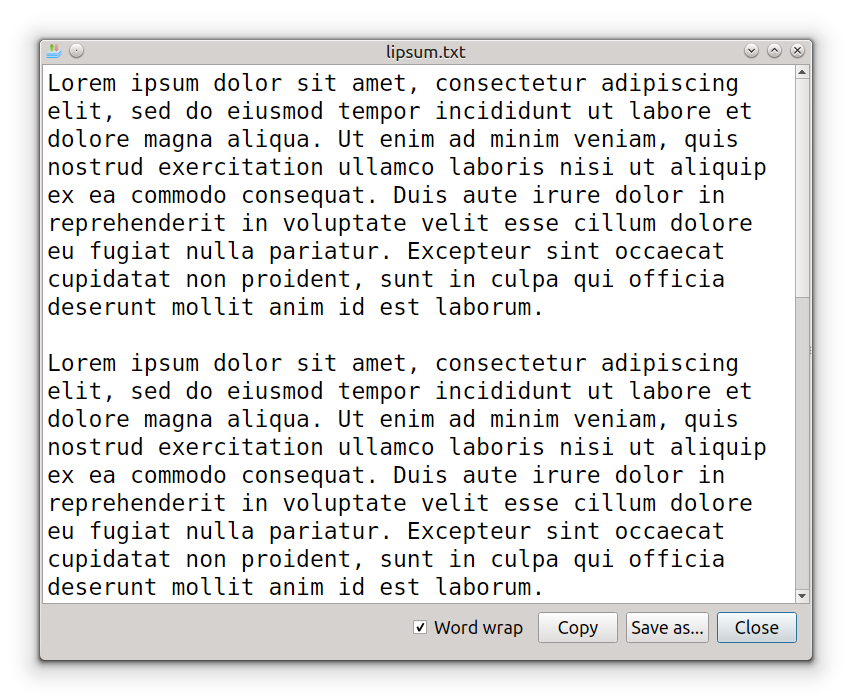
\includegraphics[scale=0.6]{images/textviewer.png}
\caption{Text viewer window}
\label{fig:textviewer}
\end{figure}

%%%%%%%%%%%%%%%%%%%%%%%%%%%%%%
% Constructor
%%%%%%%%%%%%%%%%%%%%%%%%%%%%%%

\begin{luafuncprototype}
gui.createdialog("textviewer" [, title])
\end{luafuncprototype}

\begin{funcdescr}
	Creates a text viewer dialog.
\end{funcdescr}

\begin{funcparams}
	\funcparam{title} (\luatype{string}, optional): window title
\end{funcparams}

\begin{funcret}
	Returns a \objtype{TextViewer} type object.
\end{funcret}

%%%%%%%%%%%%%%%%%%%%%%%%%%%%%%
% form.setfont()
%%%%%%%%%%%%%%%%%%%%%%%%%%%%%%

\begin{luafuncprototype}
\emph{textviewer}.setfont(name [, size [, subfamily]])
\end{luafuncprototype}

\begin{funcdescr}
	Sets the font used to display text.
\end{funcdescr}

\begin{funcparams}
	\funcparam{name} (\luatype{string}): font name (see the Remarks section below)
	\funcparam{size} (\luatype{number}, optional): point size
	\funcparam{subfamily} (\luatype{string}, optional): font subfamily (\luaexpr{"regular"}, \luaexpr{"italic"}, \luaexpr{"bold"} or \luaexpr{"bold italic"})
\end{funcparams}

\begin{funcremarks}
	\luaexpr{name} can be either a font family name, like \luaexpr{"Times"}, \luaexpr{"Helvetica"} or \luaexpr{"Courier"}, or one of the special values listed below:
	
	\begin{itemize}
		\item \luaexpr{"default"}: default user interface font
		\item \luaexpr{"sans-serif"}: default sans-serif font
		\item \luaexpr{"serif"}: default serif font
		\item \luaexpr{"monospace"}: default fixed width font
	\end{itemize}
\end{funcremarks}

%%%%%%%%%%%%%%%%%%%%%%%%%%%%%%
% form.settext()
%%%%%%%%%%%%%%%%%%%%%%%%%%%%%%

\begin{luafuncprototype}
\emph{textviewer}.settext(text)
\end{luafuncprototype}

\begin{funcdescr}
	Replaces window contents with \luaexpr{text}.
\end{funcdescr}

\begin{funcparams}
	\funcparam{text} (\luatype{string}): text to display
\end{funcparams}

%%%%%%%%%%%%%%%%%%%%%%%%%%%%%%
% form.addtext()
%%%%%%%%%%%%%%%%%%%%%%%%%%%%%%

\begin{luafuncprototype}
\emph{textviewer}.addtext(text)
\end{luafuncprototype}

\begin{funcdescr}
	Adds \luaexpr{text} to the window.
\end{funcdescr}

\begin{funcparams}
	\funcparam{text} (\luatype{string}): text to add
\end{funcparams}

%%%%%%%%%%%%%%%%%%%%%%%%%%%%%%
% form.setfile()
%%%%%%%%%%%%%%%%%%%%%%%%%%%%%%

\begin{luafuncprototype}
\emph{textviewer}.setfile(filename)
\end{luafuncprototype}

\begin{funcdescr}
	Replaces window contents with the data from \luaexpr{filename}.
\end{funcdescr}

\begin{funcparams}
	\funcparam{filename} (\luatype{string}): file name
\end{funcparams}

%%%%%%%%%%%%%%%%%%%%%%%%%%%%%%
% form.setwrap()
%%%%%%%%%%%%%%%%%%%%%%%%%%%%%%

\begin{luafuncprototype}
\emph{textviewer}.setwrap(mode)
\end{luafuncprototype}

\begin{funcdescr}
	Sets the word wrap mode.
\end{funcdescr}

\begin{funcparams}
	\funcparam{mode} (\luatype{boolean}): word wrap mode (true to wrap lines at word boundaries, false otherwise)
\end{funcparams}

%%%%%%%%%%%%%%%%%%%%%%%%%%%%%%
% form.clear()
%%%%%%%%%%%%%%%%%%%%%%%%%%%%%%

\begin{luafuncprototype}
\emph{textviewer}.clear()
\end{luafuncprototype}

\begin{funcdescr}
	Clears the window.
\end{funcdescr}

%%%%%%%%%%%%%%%%%%%%%%%%%%%%%%
% Common methods
%%%%%%%%%%%%%%%%%%%%%%%%%%%%%%

\begin{luafuncprototype}
\emph{textviewer}.show([action]) \\
\emph{textviewer}.close() \\
\emph{textviewer}.settitle([title]) \\
\emph{textviewer}.resize([width, height]) \\
\emph{textviewer}.move(...)
\end{luafuncprototype}

\begin{funcdescr}
	See Subsection \ref{subsec:luamodelessdialog}.
\end{funcdescr}

\subsection{\objtype{Plotter} type object}
\label{subsec:luaplotter}

A plotter is used to display numerical data in a graphic form. While not technically a dialog, it is also created by the \luaexpr{gui.createdialog()} function and supports the common modeless dialog interface. An example is shown on Figure \ref{fig:luaplotter}.

\begin{shellcmds}\begin{luacode}
plotter=gui.createdialog("plotter")
plotter.adddata({1,10,2,9,3,8,4,7,5,6})
\end{luacode}\end{shellcmds}

\begin{figure}[htbp]
\centering
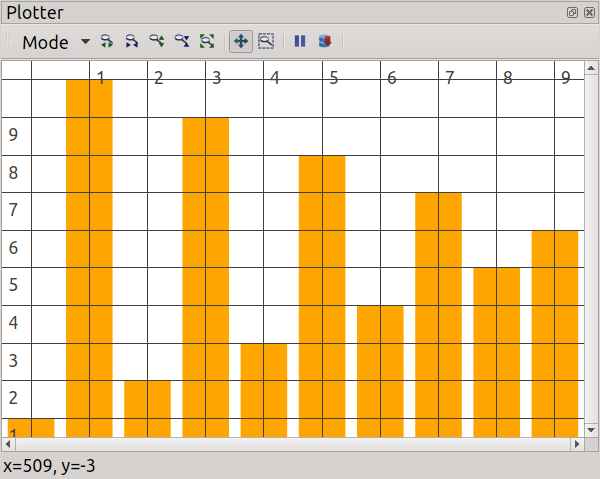
\includegraphics{images/luaplotter.png}
\caption{Plotter window}
\label{fig:luaplotter}
\end{figure}

%%%%%%%%%%%%%%%%%%%%%%%%%%%%%%
% Constructor
%%%%%%%%%%%%%%%%%%%%%%%%%%%%%%

\begin{luafuncprototype}
gui.createdialog("plotter" [, mode])
\end{luafuncprototype}

\begin{funcdescr}
	Creates a plotter window.
\end{funcdescr}

\begin{funcparams}
	\funcparam{mode} (\luatype{string}, optional): data representation mode:
	\begin{itemize}
		\item \expr{preferred} (either \luaexpr{"bars"} or \luaexpr{"plot"}, depending on the last user choice; this is the default mode)
		\item \expr{bars} (a bar chart)
		\item \expr{plot} (an ordinary 2D graph)
		\item \expr{bitmap} (a multi-line bitmap)
		\item \expr{video} (two-dimensional video data)
		\item \expr{binary} (multi-line binary data)
	\end{itemize}
\end{funcparams}

\begin{funcret}
	Returns a \objtype{Plotter} type object.
\end{funcret}

%%%%%%%%%%%%%%%%%%%%%%%%%%%%%%
% plotter.adddata()
%%%%%%%%%%%%%%%%%%%%%%%%%%%%%%

\begin{luafuncprototype}
\emph{plotter}.adddata(data [, layer])
\end{luafuncprototype}

\begin{funcdescr}
	Adds a line of data to the plot.
\end{funcdescr}

\begin{funcparams}
	\funcparam{data} (\luatype{table}): data to add
	\funcparam{layer} (\luatype{integer}, optional): layer (default is \luaexpr{0})
\end{funcparams}

\begin{funcremarks}
	In \luaexpr{"bars"} and \luaexpr{"plot"} modes the plotter can draw multiple layers, but only one line at a time (adding a new line erases the previous one). In \luaexpr{"bitmap"} and \luaexpr{"binary"} modes it can draw multiple lines, but only one layer. In \luaexpr{"video"} mode plotter displays a single layer and a single packet of data which is split into multiple lines according to the video width set by the user (or \luaexpr{setoption} method). To create a new layer in the \luaexpr{"bitmap"}, \luaexpr{"video"} or \luaexpr{"binary"} mode, the existing layer must be removed first (see the \luaexpr{removedata()} method).
\end{funcremarks}

%%%%%%%%%%%%%%%%%%%%%%%%%%%%%%
% plotter.removedata()
%%%%%%%%%%%%%%%%%%%%%%%%%%%%%%

\begin{luafuncprototype}
\emph{plotter}.removedata([count [, layer]])
\end{luafuncprototype}

\begin{funcdescr}
	Removes last \luaexpr{count} lines of data from the plot's \luaexpr{layer}. If \luaexpr{count} equals \luaexpr{-1} or is equal or greater than the number of stored lines, the entire layer is removed.
\end{funcdescr}

\begin{funcparams}
	\funcparam{count} (\luatype{integer}, optional): number of lines to remove (default is \luaexpr{-1}, that is, remove the entire layer)
	\funcparam{layer} (\luatype{integer}, optional): layer (default is \luaexpr{0})
\end{funcparams}

%%%%%%%%%%%%%%%%%%%%%%%%%%%%%%
% plotter.setmode()
%%%%%%%%%%%%%%%%%%%%%%%%%%%%%%

\begin{luafuncprototype}
\emph{plotter}.setmode([mode])
\end{luafuncprototype}

\begin{funcdescr}
	Queries a current data representation mode and optionally sets it.
\end{funcdescr}

\begin{funcparams}
	\funcparam{mode} (\luatype{string}, optional): new mode (\luaexpr{"preferred"}, \luaexpr{"bars"}, \luaexpr{"plot"}, \luaexpr{"bitmap"}, \luaexpr{"video"} or \luaexpr{"binary"})
\end{funcparams}

\begin{funcret}
	Returns the previous mode.
\end{funcret}

%%%%%%%%%%%%%%%%%%%%%%%%%%%%%%
% plotter.setoption()
%%%%%%%%%%%%%%%%%%%%%%%%%%%%%%

\begin{luafuncprototype}
\emph{plotter}.setoption(name [, value])
\end{luafuncprototype}

\begin{funcdescr}
	Queries a plotter option \luaexpr{name} and optionally sets it to \luaexpr{value}.
\end{funcdescr}

\begin{funcparams}
	\funcparam{name} (\luatype{string}): option name (see the \emph{Remarks} below)
	\funcparam{value} (type depends on \luaexpr{name}, optional): a value to set
\end{funcparams}

\begin{funcret}
	Returns the previous option value.
\end{funcret}

\begin{funcremarks}
	A list of possible options depends on \luaexpr{mode}.
	
	\luaexpr{"bars"} and \luaexpr{"plot"} modes define the following option:
	
	\begin{itemize}
		\item \luaexpr{"linewidth"} (\luatype{integer}): line width for the \luaexpr{"plot"} mode
		\item \luaexpr{"antialiasing"} (\luatype{bool}): use antialiasing for the \luaexpr{"plot"} mode
	\end{itemize}
	
	Note that while these options can be set for both \luaexpr{"bars"} and \luaexpr{"plot"} modes, they are only used by the \luaexpr{"plot"} mode. Line width of 0 (the default value) instructs the plotter to use a cosmetic pen, which is 1 pixel wide when rasterized on the screen, but can be different when exported to vector formats (SVG or PDF).
	
	\luaexpr{"bitmap"} mode defines the following options:
	
	\begin{itemize}
		\item \luaexpr{"lines"} (\luatype{integer}): number of lines to display
		\item \luaexpr{"blackpoint"} (\luatype{number}): black point value
		\item \luaexpr{"whitepoint"} (\luatype{number}): white point value
		\item \luaexpr{"inverty"} (\luatype{boolean}): invert Y axis
	\end{itemize}

	\luaexpr{"video"} mode defines the following options:
	
	\begin{itemize}
		\item \luaexpr{"blackpoint"} (\luatype{number}): black point value
		\item \luaexpr{"whitepoint"} (\luatype{number}): white point value
		\item \luaexpr{"videowidth"} (\luatype{boolean}): video width
	\end{itemize}

	\luaexpr{"binary"} mode defines the following options:
	
	\begin{itemize}
		\item \luaexpr{"lines"} (\luatype{integer}): number of lines to display
		\item \luaexpr{"bits"} (\luatype{integer}): number of significant bits per sample
		\item \luaexpr{"lsbfirst"} (\luatype{boolean}): put the least significant bit first
		\item \luaexpr{"inverty"} (\luatype{boolean}): invert Y axis
	\end{itemize}
\end{funcremarks}

%%%%%%%%%%%%%%%%%%%%%%%%%%%%%%
% plotter.setlayeroption()
%%%%%%%%%%%%%%%%%%%%%%%%%%%%%%

\begin{luafuncprototype}
\emph{plotter}.setlayeroption(layer, name [, value])
\end{luafuncprototype}

\begin{funcdescr}
	Queries a layer option \luaexpr{name} and optionally sets it to \luaexpr{value}.
\end{funcdescr}

\begin{funcparams}
	\funcparam{layer} (\luatype{integer}): layer
	\funcparam{name} (\luatype{string}): option name (see the \emph{Remarks} below)
	\funcparam{value} (type depends on \luaexpr{name}, optional): a value to set
\end{funcparams}

\begin{funcret}
	Returns the previous layer option value.
\end{funcret}

\begin{funcremarks}
	All modes support the following layer options:
	
	\begin{itemize}
		\item \luaexpr{"name"} (\luatype{string}): layer display name
		\item \luaexpr{"visibility"} (\luatype{boolean}): layer visibility
	\end{itemize}
	
	In \luaexpr{"bars"} and \luaexpr{"plot"} modes any number of layers can be visible; in other modes, only one layer can be visible at any time (making another layer visible hides the currently visible layer).
	
	In addition, \luaexpr{"bars"} and \luaexpr{"plot"} modes support the following layer options:
	
	\begin{itemize}
		\item \luaexpr{"scale"} (\luatype{number}): layer transformation scale
		\item \luaexpr{"inputoffset"} (\luatype{number}): layer transformation input offset
		\item \luaexpr{"outputoffset"} (\luatype{number}): layer transformation output offset
		\item \luaexpr{"color"} (\luatype{string}): layer color name
	\end{itemize}

	Layer transformation is based on the following formula:
	
\begin{displaymath}
y = \mathit{scale} \cdot (x + \mathit{inputOffset}) + \mathit{outputOffset}
\end{displaymath}
	
	Color names can be represented as in HTML or CSS (\luaexpr{"\#RRGGBB"}), SVG named colors are also supported\footnote{\url{https://www.w3.org/TR/SVG/types.html\#ColorKeywords}}.
\end{funcremarks}

%%%%%%%%%%%%%%%%%%%%%%%%%%%%%%
% plotter.zoom()
%%%%%%%%%%%%%%%%%%%%%%%%%%%%%%

\begin{luafuncprototype}
\emph{plotter}.zoom([x, y])
\end{luafuncprototype}

\begin{funcdescr}
	Changes plotter window display scale.
\end{funcdescr}

\begin{funcparams}
	\funcparam{x} (\luatype{number}, optional): x scale ratio
	\funcparam{y} (\luatype{number}, optional): y scale ratio
\end{funcparams}

\begin{funcremarks}
	When called without arguments, fits the whole image in the window (equivalent to the \uielement{Zoom fit} toolbar button).
	
	When called with \luaexpr{x} and \luaexpr{y} arguments, multiplies the horizontal and vertical scale coefficients by \luaexpr{x} and \luaexpr{y} respectively.
\end{funcremarks}

%%%%%%%%%%%%%%%%%%%%%%%%%%%%%%
% plotter.addcursor()
%%%%%%%%%%%%%%%%%%%%%%%%%%%%%%

\begin{luafuncprototype}
\emph{plotter}.addcursor(pos [, name])
\end{luafuncprototype}

\begin{funcdescr}
	Adds a cursor to the plotter window.
\end{funcdescr}

\begin{funcparams}
	\funcparam{pos} (\luatype{integer}): cursor position
	\funcparam{name} (\luatype{string}, optional): cursor name
\end{funcparams}

%%%%%%%%%%%%%%%%%%%%%%%%%%%%%%
% Common methods
%%%%%%%%%%%%%%%%%%%%%%%%%%%%%%

\begin{luafuncprototype}
\emph{plotter}.show([action]) \\
\emph{plotter}.close() \\
\emph{plotter}.settitle([title]) \\
\emph{plotter}.resize([width, height]) \\
\emph{plotter}.move(...)
\end{luafuncprototype}

\begin{funcdescr}
	See Subsection \ref{subsec:luamodelessdialog}. Note that window management functions such as \luaexpr{resize()} and \luaexpr{move()} will not work properly when the plotter window is docked.
\end{funcdescr}

\section[codec library]{\expr{codec} library}

\expr{codec} library handles text encoding conversion. Its features are accessed through the \expr{codec} global object of \objtype{Codec} type.

SDM internally uses UTF-8 to represent all text. Native UTF-8 support provided by Lua is limited: it can work with UTF-8 strings as byte arrays and convert them to arrays of code points (since Lua 5.3), but for all interactions with the operating system (file names, environment variables, etc.) a locale-dependent multibyte encoding is used. This is not usually a problem for Linux since it likely uses UTF-8 anyway, but Windows uses legacy ``ANSI'' and ``OEM'' encodings which can't represent all Unicode characters. On the other hand, Windows provides a separate UTF-16 API, but standard Lua libraries make no use of it.

The functions of the \expr{codec} library are provided to partially mitigate the aforementioned encoding problems. Some of them, like \luaexpr{codec.dofile()} and \luaexpr{codec.open()}, are designed to be replacements for the similar functions from the Lua standard library. The standard functions are not replaced by default; if desired, one can replace them as follows:

\begin{shellcmds}\begin{luacode}
dofile=codec.dofile
io.open=codec.open
\end{luacode}\end{shellcmds}

\subsection{\expr{codec} global object}
\label{subsec:codec}

%%%%%%%%%%%%%%%%%%%%%%%%%%%%%%
% codec.utf8tolocal()
%%%%%%%%%%%%%%%%%%%%%%%%%%%%%%

\begin{luafuncprototype}
codec.utf8tolocal(str)
\end{luafuncprototype}

\begin{funcdescr}
	Converts a UTF-8 string to a locale-dependent multibyte encoding.
\end{funcdescr}

\begin{funcparams}
	\funcparam{str} (\luatype{string}): a UTF-8 string
\end{funcparams}

\begin{funcret}
	Returns the converted string.
\end{funcret}

\begin{funcremarks}
	More advanced text encoding conversion features are provided by the codec FSM (Subsection \ref{subsec:codecfsm}).
\end{funcremarks}

%%%%%%%%%%%%%%%%%%%%%%%%%%%%%%
% codec.localtoutf8()
%%%%%%%%%%%%%%%%%%%%%%%%%%%%%%

\begin{luafuncprototype}
codec.localtoutf8(str)
\end{luafuncprototype}

\begin{funcdescr}
	Converts a string in a locale-dependent multibyte encoding to a UTF-8 string.
\end{funcdescr}

\begin{funcparams}
	\funcparam{str} (\luatype{string}): a string in local encoding
\end{funcparams}

\begin{funcret}
	Returns the converted string.
\end{funcret}

\begin{funcremarks}
	More advanced text encoding conversion features are provided by the codec FSM (Subsection \ref{subsec:codecfsm}).
\end{funcremarks}

%%%%%%%%%%%%%%%%%%%%%%%%%%%%%%
% codec.print(), codec.write()
%%%%%%%%%%%%%%%%%%%%%%%%%%%%%%

\begin{luafuncprototype}
codec.print(str) \\
codec.write(str)
\end{luafuncprototype}

\begin{funcdescr}
	Writes a UTF-8 encoded text string to the standard output. The difference between \luaexpr{codec.print()} and \luaexpr{codec.write()} is that the former will append a newline character, while the latter won't.
\end{funcdescr}

\begin{funcparams}
	\funcparam{str} (\luatype{string}): a UTF-8 string
\end{funcparams}

\begin{funcremarks}
	Standard stream encoding is only converted when the stream is detected to be bound to a console (terminal), otherwise stream encoding is unchanged. This allows the output to be displayed correctly in \shellcmd{sdmconsole} which expects UTF-8 encoded data.
\end{funcremarks}

%%%%%%%%%%%%%%%%%%%%%%%%%%%%%%
% codec.dofile()
%%%%%%%%%%%%%%%%%%%%%%%%%%%%%%

\begin{luafuncprototype}
codec.dofile([filename])
\end{luafuncprototype}

\begin{funcdescr}
	Executes a Lua script from a file with a UTF-8 encoded name. When called without arguments, reads from the standard input.
\end{funcdescr}

\begin{funcparams}
	\funcparam{filename} (\luatype{string}, optional): file name (UTF-8 encoded)
\end{funcparams}

\begin{funcret}
	Returns all values returned by the chunk (if any).
\end{funcret}

\begin{funcremarks}
	This function is similar to the \luaexpr{dofile()} function from the Lua standard library, but is not affected by Windows-related file name encoding problems since it uses wide-character API to open files, making it possible to work with file names containing characters not present in the current ANSI code page.
	
	If \luaexpr{filename} is not an absolute path, the function will use the following rules to resolve it:
	
	\begin{enumerate}
		\item If the code currently being executed originates from a file, try to resolve the path relative to the directory containing that file.
		\item Failing that, try to resolve the path relative to the SDM Lua modules directory intended for backend scripts (Section \ref{sec:installdirectories}).
		\item Failing that, try to resolve the path relative to the SDM scripts directory intended for user-visible scripts (Section \ref{sec:installdirectories}).
		\item Failing that, try resolve the path relative to the current directory.
		\item Failing that, raise an error.
	\end{enumerate}
	
	This is different from the standard \luaexpr{dofile()} behavior which is always to use the current directory.
\end{funcremarks}

%%%%%%%%%%%%%%%%%%%%%%%%%%%%%%
% codec.open()
%%%%%%%%%%%%%%%%%%%%%%%%%%%%%%

\begin{luafuncprototype}
codec.open(filename [, mode])
\end{luafuncprototype}

\begin{funcdescr}
	Opens a file with a UTF-8 encoded name.
\end{funcdescr}

\begin{funcparams}
	\funcparam{filename} (\luatype{string}): file name (UTF-8 encoded)
	\funcparam{mode} (\luatype{string}, optional): access mode, like in \luaexpr{io.open()}: \luaexpr{"r"}, \luaexpr{"w"}, \luaexpr{"a"}, \luaexpr{"r+"}, \luaexpr{"w+"} or \luaexpr{"a+"}; default is \luaexpr{"r"}; \expr{b} can be added to the mode string as a second or third character to force binary mode on Microsoft Windows
\end{funcparams}

\begin{funcret}
	Returns a file handle that is compatible with standard Lua functions from the \luaexpr{io} library, or \luaexpr{nil} and an error message in case of errors.
\end{funcret}

\begin{funcremarks}
	This function is designed to be a drop-in replacement for the standard \luaexpr{io.open()} function. Unlike the latter, this function assumes the file name to be encoded in UTF-8. Under Microsoft Windows it uses wide-character API to open files, which makes it possible to work with file names containing characters not present in the current ANSI code page.
	
	Only file names are transcoded, contents are in no way altered.
\end{funcremarks}

%%%%%%%%%%%%%%%%%%%%%%%%%%%%%%
% codec.createcodec()
%%%%%%%%%%%%%%%%%%%%%%%%%%%%%%

\begin{luafuncprototype}
codec.createcodec(encoding)
\end{luafuncprototype}

\begin{funcdescr}
	Creates a state machine for conversion between UTF-8 and the selected encoding.
\end{funcdescr}

\begin{funcparams}
	\funcparam{encoding} (\luatype{string}): see below
\end{funcparams}

\begin{funcret}
	Returns a \objtype{CodecFSM} type object.
\end{funcret}

\begin{funcremarks}
	Character encodings recognized by the library are listed in Table \ref{tab:encodings}. Some of these encodings can be unsupported on certain platforms. Hyphens and underscores in encoding names are ignored. \luaexpr{"local"} is a locale-dependent multibyte encoding, \luaexpr{"ansi"} is a synonym for \luaexpr{"local"}, \luaexpr{"oem"} is an OEM encoding on Microsoft Windows and equivalent to \luaexpr{"local"} on other platforms. \luaexpr{"utf-16"} endianness is native to the platform. \luaexpr{"wchar\_t"} is a native wide character encoding equivalent to \luaexpr{"utf-16"} on Microsoft Windows. Byte order marks (BOM) are not inserted.
	
	\begin{table}[htbp]
	\caption{Supported encodings}
	\label{tab:encodings}
	\autorows[0.8\textwidth]{c}{3}{l}{\expr{local}, \expr{ansi}, \expr{oem}, \expr{wchar\_t}, \expr{utf-8}, \expr{utf-16}, \expr{utf-16le}, \expr{utf-16be}, \expr{iso-8859-1}, \expr{iso-8859-2}, \expr{iso-8859-3}, \expr{iso-8859-4}, \expr{iso-8859-5}, \expr{iso-8859-6}, \expr{iso-8859-7}, \expr{iso-8859-8}, \expr{iso-8859-9}, \expr{iso-8859-13}, \expr{iso-8859-15}, \expr{windows-1250}, \expr{windows-1251}, \expr{windows-1252}, \expr{windows-1253}, \expr{windows-1254}, \expr{windows-1255}, \expr{windows-1256}, \expr{windows-1257}, \expr{windows-1258}, \expr{cp437}, \expr{cp850}, \expr{cp866}, \expr{koi8-r}, \expr{koi8-u}, \expr{gb2312}, \expr{gb18030}, \expr{big5}, \expr{shiftjis}, \expr{euc-jp}, \expr{euc-kr}}
	\end{table}
\end{funcremarks}

\subsection{\objtype{CodecFSM} type object}
\label{subsec:codecfsm}

\begin{funcdescr}
	\objtype{CodecFSM} implements a state-based text codec providing conversion from UTF-8 to the specified encoding and vice versa. If a data block ends with an incomplete multibyte sequence, the codec will remember its state and use it later when transcoding the next block. \objtype{CodecFSM} objects can be created using the \luaexpr{codec.createcodec()} function.
\end{funcdescr}

A simple example:

\begin{shellcmds}\begin{luacode}
fsm=codec.createcodec("utf-16le")
s=fsm.fromutf8("abc αβγ")
io.write("UTF-16 data: ")
for i=1,#s do
    io.write(string.format("%02X ",s:byte(i)))
end
\end{luacode}\end{shellcmds}

The following data will be printed:

\begin{shellcmds}
UTF-16 data: 61 00 62 00 63 00 20 00 B1 03 B2 03 B3 03
\end{shellcmds}

%%%%%%%%%%%%%%%%%%%%%%%%%%%%%%
% codecfsm.close()
%%%%%%%%%%%%%%%%%%%%%%%%%%%%%%

\begin{luafuncprototype}
\emph{codecfsm}.close()
\end{luafuncprototype}

\begin{funcdescr}
	Destroys the object.
\end{funcdescr}

%%%%%%%%%%%%%%%%%%%%%%%%%%%%%%
% codecfsm.fromutf8()
%%%%%%%%%%%%%%%%%%%%%%%%%%%%%%

\begin{luafuncprototype}
\emph{codecfsm}.fromutf8(str)
\end{luafuncprototype}

\begin{funcdescr}
	Converts \luaexpr{str} from UTF-8 to the selected encoding.
\end{funcdescr}

\begin{funcparams}
	\funcparam{str} (\luatype{string}): a UTF-8 string to convert
\end{funcparams}

\begin{funcret}
	Returns the converted string.
\end{funcret}

%%%%%%%%%%%%%%%%%%%%%%%%%%%%%%
% codecfsm.toutf8()
%%%%%%%%%%%%%%%%%%%%%%%%%%%%%%

\begin{luafuncprototype}
\emph{codecfsm}.toutf8(str)
\end{luafuncprototype}

\begin{funcdescr}
	Converts \luaexpr{str} from the selected encoding to UTF-8.
\end{funcdescr}

\begin{funcparams}
	\funcparam{str} (\luatype{string}): a string to convert
\end{funcparams}

\begin{funcret}
	Returns the converted string.
\end{funcret}

%%%%%%%%%%%%%%%%%%%%%%%%%%%%%%
% codecfsm.reset()
%%%%%%%%%%%%%%%%%%%%%%%%%%%%%%

\begin{luafuncprototype}
\emph{codecfsm}.reset([direction])
\end{luafuncprototype}

\begin{funcdescr}
	Resets the codec state.
\end{funcdescr}

\begin{funcparams}
	\funcparam{direction} (\luatype{string}, optional): \luaexpr{"fromutf8"}, \luaexpr{"toutf8"} or \luaexpr{"both"}; default is \luaexpr{"both"}
\end{funcparams}

\section[RegisterMap type object]{\objtype{RegisterMap} type object}
\label{sec:luaregistermap}

Unlike most \shellcmd{sdmconsole} GUI objects, \objtype{RegisterMap} objects are not created by the \expr{gui} library. Instead, they are produced using the \luaexpr{registermap()} method of the \objtype{Channel} type object (Subsection \ref{subsec:luachannel}).

%%%%%%%%%%%%%%%%%%%%%%%%%%%%%%
% map.pages()
%%%%%%%%%%%%%%%%%%%%%%%%%%%%%%

\begin{luafuncprototype}
\emph{map}.pages()
\end{luafuncprototype}

\begin{funcret}
	Returns number of pages in the register map.
\end{funcret}

%%%%%%%%%%%%%%%%%%%%%%%%%%%%%%
% map.addpage()
%%%%%%%%%%%%%%%%%%%%%%%%%%%%%%

\begin{luafuncprototype}
\emph{map}.addpage([name])
\end{luafuncprototype}

\begin{funcdescr}
	Adds a new page to the register map.
\end{funcdescr}

\begin{funcparams}
	\funcparam{name} (\luatype{string}, optional): page name
\end{funcparams}

\begin{funcret}
	Returns the index of the created page (counted from 1).
\end{funcret}

%%%%%%%%%%%%%%%%%%%%%%%%%%%%%%
% map.removepage()
%%%%%%%%%%%%%%%%%%%%%%%%%%%%%%

\begin{luafuncprototype}
\emph{map}.removepage([index])
\end{luafuncprototype}

\begin{funcdescr}
	Removes the page with index \luaexpr{index} (counted from 1).
\end{funcdescr}

\begin{funcparams}
	\funcparam{index} (\luatype{integer}): index of the page to remove
\end{funcparams}

%%%%%%%%%%%%%%%%%%%%%%%%%%%%%%
% map.pagename()
%%%%%%%%%%%%%%%%%%%%%%%%%%%%%%

\begin{luafuncprototype}
\emph{map}.pagename(index [, name])
\end{luafuncprototype}

\begin{funcdescr}
	Queries the name of the page \luaexpr{index}, optionally sets it.
\end{funcdescr}

\begin{funcparams}
	\funcparam{index} (\luatype{integer}): page index
	\funcparam{name} (\luatype{string}, optional): a name to set
\end{funcparams}

\begin{funcret}
	Returns the previous page name.
\end{funcret}

%%%%%%%%%%%%%%%%%%%%%%%%%%%%%%
% map.rows()
%%%%%%%%%%%%%%%%%%%%%%%%%%%%%%

\begin{luafuncprototype}
\emph{map}.rows(index)
\end{luafuncprototype}

\begin{funcdescr}
	Queries the number of rows for the page \luaexpr{index}.
\end{funcdescr}

\begin{funcparams}
	\funcparam{index} (\luatype{integer}): page index
\end{funcparams}

\begin{funcret}
	Returns the number of rows.
\end{funcret}

%%%%%%%%%%%%%%%%%%%%%%%%%%%%%%
% map.insertrow()
%%%%%%%%%%%%%%%%%%%%%%%%%%%%%%

\begin{luafuncprototype}
\emph{map}.insertrow(page, row, data)
\end{luafuncprototype}

\begin{funcdescr}
	Inserts a new row.
\end{funcdescr}

\begin{funcparams}
	\funcparam{page} (\luatype{integer}): page index
	\funcparam{row} (\luatype{integer}): row index
	\funcparam{data} (\luatype{table}): row data
\end{funcparams}

\begin{funcremarks}
	Row data table contains the following fields:
	\begin{itemize}
		\item For all row types:
		\begin{itemize}
			\item \luaexpr{name} (\luatype{string}): section, register or FIFO name;
			\item \expr{type} (\luatype{string}): \luaexpr{"section"}, \luaexpr{"register"}, \luaexpr{"fifo"} or \luaexpr{"memory"}.
		\end{itemize}
		\item For \uielement{Register}, \uielement{FIFO} and \uielement{Memory} type rows:
		\begin{itemize}
			\item \luaexpr{id} (\luatype{string}): optional identifier (can be absent);
			\item \luaexpr{addr} (\luatype{integer}): register address (can be absent);
			\item \luaexpr{data} (\luatype{integer} for register, \luatype{table} for FIFO or memory): register or FIFO/memory data, can be absent;
			\item \luaexpr{writeaction} (\luatype{string}): custom write action (if defined);
			\item \luaexpr{readaction} (\luatype{string}): custom read action (if defined);
			\item \luaexpr{skipgroupwrite} (\luatype{boolean}): skip this row when writing multiple rows;
			\item \luaexpr{skipgroupread} (\luatype{boolean}): skip this row when reading multiple rows.
		\end{itemize}
		\item Only for \uielement{Register} type rows:
		\begin{itemize}
			\item \luaexpr{widget} (\luatype{string}): widget type for data column (\luaexpr{"lineedit"}, \luaexpr{"dropdown"}, \luaexpr{"combobox"} or \luaexpr{"pushbutton"});
			\item \luaexpr{options} (\luatype{table}): a table of options for a drop-down list, a combobox or a push button. Table items are themselves tables containing \luaexpr{name} and \luaexpr{value} fields.
		\end{itemize}
		\item Only for \uielement{FIFO} and \uielement{Memory} type rows:
		\begin{itemize}
			\item \luaexpr{prewriteaddr} (\luatype{integer}): indirect addressing register
			\item \luaexpr{prewritedata} (\luatype{integer}): indirect addressing data
		\end{itemize}
	\end{itemize}
\end{funcremarks}

%%%%%%%%%%%%%%%%%%%%%%%%%%%%%%
% map.removerow()
%%%%%%%%%%%%%%%%%%%%%%%%%%%%%%

\begin{luafuncprototype}
\emph{map}.removerow(page, row)
\end{luafuncprototype}

\begin{funcdescr}
	Removes an existing row.
\end{funcdescr}

\begin{funcparams}
	\funcparam{page} (\luatype{integer}): page index
	\funcparam{row} (\luatype{integer}): row index
\end{funcparams}

%%%%%%%%%%%%%%%%%%%%%%%%%%%%%%
% map.rowdata()
%%%%%%%%%%%%%%%%%%%%%%%%%%%%%%

\begin{luafuncprototype}
\emph{map}.rowdata(page, row [, data])
\end{luafuncprototype}

\begin{funcdescr}
	Queries, and optionally sets, data for the specified row.
\end{funcdescr}

\begin{funcparams}
	\funcparam{page} (\luatype{integer}): page index
	\funcparam{row} (\luatype{integer}): row index
	\funcparam{data} (\luatype{table}, optional): data to set (see the \luaexpr{insertrow()} method description)
\end{funcparams}

%%%%%%%%%%%%%%%%%%%%%%%%%%%%%%
% map.currentpage()
%%%%%%%%%%%%%%%%%%%%%%%%%%%%%%

\begin{luafuncprototype}
\emph{map}.currentpage()
\end{luafuncprototype}

\begin{funcret}
	Returns the index of the current page.
\end{funcret}

%%%%%%%%%%%%%%%%%%%%%%%%%%%%%%
% map.currentrow()
%%%%%%%%%%%%%%%%%%%%%%%%%%%%%%

\begin{luafuncprototype}
\emph{map}.currentrow()
\end{luafuncprototype}

\begin{funcret}
	Returns the index of the current (selected) row.
\end{funcret}

%%%%%%%%%%%%%%%%%%%%%%%%%%%%%%
% map.findrow()
%%%%%%%%%%%%%%%%%%%%%%%%%%%%%%

\begin{luafuncprototype}
\emph{map}.findrow(value, how)
\end{luafuncprototype}

\begin{funcdescr}
	Searches a row in the register map.
\end{funcdescr}

\begin{funcparams}
	\funcparam{value} (\luatype{string}): value to search for
	\funcparam{how} (\luatype{string}): type of search: \luaexpr{"name"}, \luaexpr{"id"} or \luaexpr{"addr"}
\end{funcparams}

\begin{funcret}
	If nothing was found, returns \luaexpr{nil}. If a suitable row was found, returns three values: row data table (see the \luaexpr{insertrow()} method description), page index and row index.
\end{funcret}

%%%%%%%%%%%%%%%%%%%%%%%%%%%%%%
% map.clear()
%%%%%%%%%%%%%%%%%%%%%%%%%%%%%%

\begin{luafuncprototype}
\emph{map}.clear()
\end{luafuncprototype}

\begin{funcdescr}
	Clears the register map.
\end{funcdescr}

%%%%%%%%%%%%%%%%%%%%%%%%%%%%%%
% map.load()
%%%%%%%%%%%%%%%%%%%%%%%%%%%%%%

\begin{luafuncprototype}
\emph{map}.load(filename)
\end{luafuncprototype}

\begin{funcdescr}
	Loads register map contents from a file.
\end{funcdescr}

\begin{funcparams}
	\funcparam{filename} (\luatype{string}): file name
\end{funcparams}

\begin{funcremarks}
	If \luaexpr{filename} is not an absolute path, it will be resolved relative to the current directory or, failing that, the SDM data directory (Section \ref{sec:installdirectories}).
\end{funcremarks}

%%%%%%%%%%%%%%%%%%%%%%%%%%%%%%
% map.save()
%%%%%%%%%%%%%%%%%%%%%%%%%%%%%%

\begin{luafuncprototype}
\emph{map}.save(filename)
\end{luafuncprototype}

\begin{funcdescr}
	Saves register map contents to a file.
\end{funcdescr}

\begin{funcparams}
	\funcparam{filename} (\luatype{string}): file name
\end{funcparams}

\section[luadfic extension module]{\expr{luadfic} extension module}

\expr{luadfic} (Dynamic Function Interface Compiler) is an extension module allowing the user to access functions exported by external shared libraries (\shellcmd{.dll} or \shellcmd{.so}). This feature is sometimes called a \emph{foreign function interface}. \expr{luadfic} is developed as a part of the SDM project, but can be also used with a standalone Lua interpreter or with any program that can use Lua extension modules. Only x86 and x86-64 based machines are currently supported by \expr{luadfic}.

\expr{luadfic} is not loaded automatically; to load it, use the \luaexpr{require()} Lua function.

\expr{luadfic} is a low-level library which by design is able to circumvent most safety mechanisms. Incorrect usage will almost certainly result in program crashes.

The following example imports the \cexpr{getenv()} function from the Standard C library:

\begin{shellcmds}\begin{luacode}
dfic=require("luadfic")
getenv=dfic.import(nil, "getenv", "char *@const char *")
path=getenv("PATH")
print(path)
\end{luacode}\end{shellcmds}

The first argument to the \luaexpr{dfic.import()} method is a library name; \luaexpr{nil} means that the symbol will be searched among the libraries already loaded by the current process (this example assumes that the program uses a shared version of the Standard C library).

\subsection{Function prototypes}
\label{subsec:dficprototypes}

The \luaexpr{import()} method has three string parameters: library file name, exported symbol name (on Microsoft Windows, functions can be also imported by a numeric identifier known as \emph{ordinal}) and function prototype. Prototype string can have one of the following formats:

\begin{alltt}
\emph{parameters}
\emph{return\_value}@\emph{parameters}
\emph{return\_value}@\emph{calling\_convention}@\emph{parameters}
\end{alltt}

\expr{\emph{parameters}} is a comma-separated list of parameter types (see below) which can be empty or \cexpr{void} if a function doesn't have any parameters. \expr{\emph{return\_value}} specifies the return value type (and can be empty or \cexpr{void} if a function doesn't return a value). \expr{\emph{calling\_convention}} specifies the calling convention; when empty, the default one is used (see Table \ref{tab:dficconventions}).

For functions that have neither parameters nor return value, empty or \luaexpr{nil} prototype string can be supplied.

\begin{table}[htbp]
	\caption{Supported calling conventions}
	\label{tab:dficconventions}
	\begin{tabularx}{\textwidth}{lL}
		\toprule
		Name & Description \\
		\midrule
		\tabcutin{2}{x86 calling conventions} \\
		\midrule
		
		\expr{cdecl} & Default. Arguments are pushed on the stack in reverse order (that is, the first argument has the lowest address), stack cleanup is a responsibility of the caller. \\
		\expr{pascal} & Arguments are pushed on the stack in direct order, stack cleanup is a responsibility of the callee. \\
		\expr{stdcall} & Arguments are pushed on the stack in reverse order, stack cleanup is a responsibility of the callee. \\
		\expr{fastcall} & The first two non-floating point arguments are passed via the \expr{ECX} and \expr{EDX} registers, others are pushed on the stack in reverse order, stack cleanup is a responsibility of the callee. \\
		\expr{thiscall} & The first argument, \cexpr{this} pointer, is passed via the \expr{ECX} register, the remaining arguments are pushed on the stack in reverse order, stack cleanup is a responsibility of the callee. \\
		\expr{winapi} & Equivalent to \expr{stdcall}. \\
		
		\midrule
		\tabcutin{2}{x86-64 calling conventions} \\
		\midrule
		
		\expr{x64} & Calling convention native to the OS. Microsoft x64 ABI is described in \emph{x64 Software Conventions}; Linux uses the ABI defined in the \emph{System V Application Binary Interface AMD64 Architecture Processor Supplement}. \\
		\expr{winapi} & Equivalent to \expr{x64}. \\
		\bottomrule
	\end{tabularx}
\end{table}

Types of parameters and return values are specified in the following form:

\vspace{\baselineskip}
\expr{[\textbf{const}] \emph{fundamental\_type} [*]}
\vspace{\baselineskip}

Conceptually, fundamental types are first-class types that have direct Lua counterparts. Supported fundamental types are listed in Table \ref{tab:dfictypes}. Synonyms are given in parentheses. Lua types for \cexpr{clock_t} and \cexpr{time_t} are platform-dependent.

\begin{table}[htbp]
	\caption{Supported fundamental types}
	\label{tab:dfictypes}
	\begin{tabularx}{\textwidth}{Ll}
		\toprule
		DFIC fundamental type & Lua type \\
		\midrule
		\expr{void\,*} & \luatype{lightuserdata} \\
		\expr{bool} & \luatype{boolean} \\
		\expr{char} (\expr{unsigned char}, \expr{signed char}) & \luatype{string} \\
		\expr{wchar\_t} & \luatype{integer} \\
		\expr{short int} (\expr{short}, \expr{signed short}, \expr{signed short int}) & \luatype{integer} \\
		\expr{unsigned short int} (\expr{unsigned short}) & \luatype{integer} \\
		\expr{int} (\expr{signed}, \expr{signed int}) & \luatype{integer} \\
		\expr{unsigned int} (\expr{unsigned}) & \luatype{integer} \\
		\expr{long int} (\expr{long}, \expr{signed long}, \expr{signed long int}) & \luatype{integer} \\
		\expr{unsigned long int} (\expr{unsigned long}) & \luatype{integer} \\
		\expr{long long int} (\expr{long long}, \expr{signed long long}, \expr{signed long long int}) & \luatype{integer} \\
		\expr{unsigned long long int} (\expr{unsigned long long}) & \luatype{integer} \\
		\expr{size\_t} & \luatype{integer} \\
		\expr{intptr\_t} & \luatype{integer} \\
		\expr{uintptr\_t} & \luatype{integer} \\
		\expr{ptrdiff\_t} & \luatype{integer} \\
		\expr{clock\_t} & \luatype{integer} or \luatype{number} \\
		\expr{time\_t} & \luatype{integer} or \luatype{number} \\
		\expr{int8\_t} & \luatype{integer} \\
		\expr{uint8\_t} & \luatype{integer} \\
		\expr{int16\_t} & \luatype{integer} \\
		\expr{uint16\_t} & \luatype{integer} \\
		\expr{int32\_t} & \luatype{integer} \\
		\expr{uint32\_t} & \luatype{integer} \\
		\expr{int64\_t} & \luatype{integer} \\
		\expr{uint64\_t} & \luatype{integer} \\
		\expr{float} & \luatype{number} \\
		\expr{double} & \luatype{number} \\
		\bottomrule
	\end{tabularx}
\end{table}

Asterisk (\cexpr{*}) denotes that a parameter or return value is passed by pointer; the exception is \expr{\textbf{void}\,*} which is considered a fundamental type by itself (but \expr{\textbf{void}\,**} is also a valid type specifier). \cexpr{const} informs the library that the function is not supposed to alter data referenced by the pointer; it doesn't have meaning for non-pointer types, \expr{\textbf{void}\,*} or return value types.

\subsection{Passing data by pointer: implicit buffer allocation}

To enable passing data by pointers, \expr{luadfic} implements an \emph{implicit buffer allocation} mechanism. When invoking a function with pointer parameters (except \expr{\textbf{void}\,*}), the library will perform the following operations:

\begin{enumerate}
	\item If the argument is \luaexpr{nil} or a \cexpr{NULL} \luatype{lightuserdata} (such as \luaexpr{dfic.nullptr}, see Subsection \ref{subsec:dficobject}), pass a \cexpr{NULL} pointer.
	\item Otherwise, allocate a temporary buffer:
		\begin{itemize}
			\item If the argument has an \luatype{integer} or \luatype{number} type, allocate a buffer of the specified size and initialize it with zeros.
			\item Otherwise:
				\begin{itemize}
					\item For \cexpr{char} pointers (also \cexpr{unsigned char} and \cexpr{signed char}) the argument must be of \luatype{string} type. Allocate a buffer of a size equal to the string size plus one and copy the string to the buffer (appending a terminating null character).
					\item For non-\cexpr{char} pointers the argument must be of \luatype{table} type (even if only one value is required). Allocate a buffer of a size equal to the table size and copy the table contents to the buffer.
				\end{itemize}
		\end{itemize}
	\item Invoke the function, passing pointers to temporary buffers as arguments.
	\item For non-\cexpr{const}, non-\cexpr{NULL} pointers, copy the contents from the buffers and pass them to the user as return values (of \luatype{string} type for \cexpr{char} pointers, of \luatype{table} type otherwise). For non-\cexpr{const} \cexpr{NULL} pointers, pass \luaexpr{nil} as a respective return value.
\end{enumerate}

\expr{luadfic} assumes that \cexpr{char} pointers reference null-terminated strings. If a fixed buffer size is needed, use explicit buffers (see the next subsection).

Suppose that we want to get a value from the Windows registry. It can be done with the \cexpr{RegGetValueA()} function from \shellcmd{advapi32.dll} which is defined as follows (Windows API macros are decoded in comments):

\begin{breakshellcmds}\begin{ccode}
LONG WINAPI RegGetValueA(   /*   long __stdcall    */
    HKEY hkey,              /*   void *            */
    LPCSTR lpSubKey,        /*   const char *      */
    LPCSTR lpValue,         /*   const char *      */
    DWORD dwFlags,          /*   unsigned long     */
    LPDWORD pdwType,        /*   unsigned long *   */
    PVOID pvData,           /*   void *            */
    LPDWORD pcbData         /*   unsigned long *   */
);
\end{ccode}\end{breakshellcmds}

The ``A'' suffix in the function name denotes that it uses ordinary narrow-character strings in a locale-dependent ``ANSI'' encoding (as opposed to UTF-16 encoded wide-character strings). \cexpr{lpSubKey}, \cexpr{lpValue}, \cexpr{pdwType}, \cexpr{pvData} and \cexpr{pcbData} parameters are passed by pointers; the last three of them point to data that are modified by the function.

The arguments that we pass to RegGetValue are:

\begin{itemize}\raggedright
	\item\luaexpr{0x80000002} for \cexpr{hKey} (\expr{HKEY\_LOCAL\_MACHINE})
	\item\luaexpr{"SOFTWARE\\\\Microsoft\\\\Windows NT\\\\CurrentVersion"} for \cexpr{lpSubKey}
	\item\luaexpr{"ProductName"} for \cexpr{lpValue}
	\item\luaexpr{2} for \cexpr{dwFlags} (restrict value type to null-terminated string)
	\item\luaexpr{nil} for \cexpr{pdwType} (indicate that \cexpr{pdwType} is not needed)
	\item\luaexpr{1024} for \cexpr{pvData} (size of the output buffer)
	\item\luaexpr{\{1024\}} for \cexpr{pcbData} (initialized with buffer size, contains output value size on return)
\end{itemize}

\begin{breakshellcmds}\begin{luacode}
dfic=require("luadfic")

RegGetValue=dfic.import("advapi32.dll", "RegGetValueA", "long@winapi@uintptr_t, const char *, const char *, unsigned long, unsigned long *, char *, unsigned long *")

r,valtype,value,count=RegGetValue(0x80000002, "SOFTWARE\\Microsoft\\Windows NT\\CurrentVersion", "ProductName", 2, nil, 1024, {1024})

print("RegGetValue returned "..r)
print("Value is "..value)
print("Value size is "..count[1])
\end{luacode}\end{breakshellcmds}

Note that the \luaexpr{count} value is passed and returned as a table, even though it has only one element.

Pointers returned by external functions are dealt with in a similar way, with the difference that \expr{luadfic} doesn't know the size of the buffer referenced by it. For \cexpr{char} pointers a null-terminated string is assumed (like in the example with \cexpr{getenv()} in the beginning of the section); otherwise a single value of the corresponding type will be extracted. If the external function returns a \cexpr{NULL} pointer, \expr{luadfic} will not try to dereference it, returning \luaexpr{nil} instead.

\subsection{Passing data by pointer: explicit buffer allocation}
\label{subsec:dficpointers2}

The other method of dealing with pointers involves explicitly allocating buffers on the heap and passing/returning \expr{\textbf{void}\,*} instead of normal pointers, since \expr{\textbf{void}\,*} doesn't participate in the implicit buffer allocation described above.

\begin{breakshellcmds}\begin{luacode}
dfic=require("luadfic")

RegGetValue=dfic.import("advapi32.dll", "RegGetValueA", "long@winapi@uintptr_t, const char *, const char *, unsigned long, unsigned long *, void *, unsigned long *")

buf=dfic.buffer(1024)

r,valtype,count=RegGetValue(0x80000002, "SOFTWARE\\Microsoft\\Windows NT\\CurrentVersion", "ProductName", 2, nil, buf.ptr(), {1024})

print("RegGetValue returned "..r)
print("Value is "..buf.read())
print("Value size is "..count[1])
\end{luacode}\end{breakshellcmds}

Note that the penultimate parameter type is declared here as \expr{\textbf{void}\,*} instead of \expr{\textbf{char}\,*}. For the other pointers implicit buffer allocation is utilized, as in the previous example.

Pointers returned by functions can also be dealt with using explicit buffers. To continue with our \cexpr{getenv()} example:

\begin{breakshellcmds}\begin{luacode}
dfic=require("luadfic")
getenv=dfic.import(nil, "getenv", "void *@const char *")
ptr=getenv("PATH")
buf=dfic.buffer(ptr,32768)
path=buf.read()
print(path)
\end{luacode}\end{breakshellcmds}

There are other operations supported by explicit buffers. See Subsection \ref{subsec:dficbuffer} for details.

\subsubsection{Working with structures}

Lua 5.3 introduced \luaexpr{string.pack()} and \luaexpr{string.unpack()} functions which can be used together with explicit buffer allocation to work with data structures. In the following example, \luaexpr{string.unpack()} is used to parse the \cexpr{tm} structure returned by \cexpr{localtime()}:

\begin{breakshellcmds}\begin{luacode}
dfic=require("luadfic")

localtime=dfic.import(nil,"localtime","void*@const time_t*")
tmptr=localtime({os.time()})

-- "struct tm" is comprised of 9 integers
buf=dfic.buffer(tmptr,9*dfic.typesize("int"))
tm=table.pack(string.unpack("iiiiiiiii",buf.read(1,#buf)))

print("tm_sec="..tm[1])
print("tm_min="..tm[2])
print("tm_hour="..tm[3])
print("tm_mday="..tm[4])
print("tm_mon="..tm[5])
print("tm_year="..tm[6])
print("tm_wday="..tm[7])
print("tm_yday="..tm[8])
print("tm_isdst="..tm[9])
\end{luacode}\end{breakshellcmds}

\subsection{\expr{dfic} global object}
\label{subsec:dficobject}

%%%%%%%%%%%%%%%%%%%%%%%%%%%%%%
% dfic.import()
%%%%%%%%%%%%%%%%%%%%%%%%%%%%%%

\begin{luafuncprototype}
dfic.import(library, symbol [, prototype])
\end{luafuncprototype}

\begin{funcdescr}
	Creates a wrapper object that can be used to invoke external function exported by \expr{symbol}.
\end{funcdescr}

\begin{funcparams}
	\funcparam{library} (\luatype{string}): shared library file name (with or without path)
	\funcparam{symbol} (\luatype{string} or \luatype{integer}): exported symbol name or ordinal
	\funcparam{prototype} (\luatype{string}, optional): function prototype (syntax is described in Subsection \ref{subsec:dficprototypes})
\end{funcparams}

\begin{funcret}
	Returns a \objtype{DficFunction} type object which can be used to invoke the function.
\end{funcret}

\begin{funcremarks}
	If \luaexpr{library} does not include a path, the dynamic linker will search for the module in standard locations defined by the platform.
	
	If loading the module fails, \expr{luadfic} will try again after appending the standard shared library extension (\expr{"dll"} on Microsoft Windows, \expr{"so"} otherwise) unless \luaexpr{library} already has one. When \luaexpr{library} is either an empty string or \luaexpr{nil}, the requested symbol will be searched among the libraries loaded by the current process.
	
	Import by ordinal is only possible on Microsoft Windows.
	
	On 32-bit Windows, if \expr{symbol} can't be found in the module, \expr{luadfic} will automatically try to apply common C-style name decoration schemes to it, like prepending symbol name with an underscore, \expr{@} sign (for the \expr{fastcall} convention) or appending \expr{@N} suffix (for \expr{fastcall} and \expr{stdcall} conventions).
	
	Note that \expr{luadfic} does not perform \cplusplus{} name decoration. Functions from \cplusplus{} libraries can still be imported, but the exact (decorated) symbol name must be supplied.
	
	When \luaexpr{prototype} is omitted, it is assumed that the function has neither parameters nor return value.
\end{funcremarks}

%%%%%%%%%%%%%%%%%%%%%%%%%%%%%%
% dfic.buffer()
%%%%%%%%%%%%%%%%%%%%%%%%%%%%%%

\begin{luafuncprototype}
dfic.buffer(size) \\
dfic.buffer(ptr, size)
\end{luafuncprototype}

\begin{funcdescr}
	Creates a \objtype{DficBuffer} type object which provides raw memory access. New or existing memory block can be used.
\end{funcdescr}

\begin{funcparams}
	\funcparam{size} (\luatype{integer}): buffer size
	\funcparam{ptr} (\luatype{lightuserdata}): pointer to the existing buffer
\end{funcparams}

\begin{funcret}
	Returns a \objtype{DficBuffer} type object.
\end{funcret}

\begin{funcremarks}
	When invoked with one argument, allocates a memory block on the heap. Allocated memory is zero-initialized. The memory block is owned by the \objtype{DficBuffer} object and will be freed when the object is destroyed (either explicitly via the \luaexpr{close()} method or by the Lua garbage collector).
	
	When invoked with two arguments, provides access to an existing buffer pointed by \expr{ptr}. \objtype{DficBuffer} object will not try to deallocate this memory.
\end{funcremarks}

%%%%%%%%%%%%%%%%%%%%%%%%%%%%%%
% dfic.info()
%%%%%%%%%%%%%%%%%%%%%%%%%%%%%%

\begin{luafuncprototype}
dfic.info(key)
\end{luafuncprototype}

\begin{funcdescr}
	Provides platform-specific information.
\end{funcdescr}

\begin{funcparams}
	\funcparam{key} (\luatype{string}): type on information requested:
	\begin{itemize}
		\item \luaexpr{"os"}: operating system type (\luaexpr{"windows"}, \luaexpr{"unix"})
		\item \luaexpr{"cpu"}: machine architecture (\luaexpr{"x86"}, \luaexpr{"x64"})
		\item \luaexpr{"extension"}: platform-dependent customary shared library extension (\luaexpr{"dll"}, \luaexpr{"so"})
	\end{itemize}
\end{funcparams}

\begin{funcret}
	Returns a string with the requested information.
\end{funcret}

%%%%%%%%%%%%%%%%%%%%%%%%%%%%%%
% dfic.typesize()
%%%%%%%%%%%%%%%%%%%%%%%%%%%%%%

\begin{luafuncprototype}
dfic.typesize(name)
\end{luafuncprototype}

\begin{funcparams}
	\funcparam{name} (\luatype{string}): name of the parameter or return value type (as in prototype string)
\end{funcparams}

\begin{funcret}
	Returns a size of the specified type (in bytes).
\end{funcret}

%%%%%%%%%%%%%%%%%%%%%%%%%%%%%%
% dfic.int2ptr()
%%%%%%%%%%%%%%%%%%%%%%%%%%%%%%

\begin{luafuncprototype}
dfic.int2ptr(i)
\end{luafuncprototype}

\begin{funcparams}
	\funcparam{i} (\luatype{integer}): integer to convert
\end{funcparams}

\begin{funcret}
	Returns a \luatype{lightuserdata} value containing pointer represented by \luaexpr{i}.
\end{funcret}

%%%%%%%%%%%%%%%%%%%%%%%%%%%%%%
% dfic.ptr2int()
%%%%%%%%%%%%%%%%%%%%%%%%%%%%%%

\begin{luafuncprototype}
dfic.ptr2int(ptr)
\end{luafuncprototype}

\begin{funcparams}
	\funcparam{ptr} (\luatype{lightuserdata}): pointer to convert
\end{funcparams}

\begin{funcret}
	Returns an \luatype{integer} value representing pointer contained by \luaexpr{ptr}.
\end{funcret}

%%%%%%%%%%%%%%%%%%%%%%%%%%%%%%
% dfic.nullptr
%%%%%%%%%%%%%%%%%%%%%%%%%%%%%%

\begin{luafuncprototype}
dfic.nullptr
\end{luafuncprototype}

\begin{funcdescr}
	A \luatype{lightuserdata} object representing a \cexpr{NULL} pointer. Note: this is not a method, but a plain data field. \expr{\textbf{void}\,*} pointers returned by external functions can be compared with this value. It can be also used as a table element value (table elements can't be \luaexpr{nil} in Lua).
\end{funcdescr}

\subsection{\objtype{DficFunction} type object}

%%%%%%%%%%%%%%%%%%%%%%%%%%%%%%
% dficfunction.close()
%%%%%%%%%%%%%%%%%%%%%%%%%%%%%%

\begin{luafuncprototype}
\emph{dficfunction}.close()
\end{luafuncprototype}

\begin{funcdescr}
	Destroys the object. If the library is not used by anything else, it is  unloaded from the process address space.
\end{funcdescr}

%%%%%%%%%%%%%%%%%%%%%%%%%%%%%%
% dficfunction.invoke()
%%%%%%%%%%%%%%%%%%%%%%%%%%%%%%

\begin{luafuncprototype}
\emph{dficfunction}(...) \\
\emph{dficfunction}.invoke(...)
\end{luafuncprototype}

\begin{funcdescr}
	Invokes an external function. Parameters are defined by the prototype.
\end{funcdescr}

\begin{funcret}
	Generally returns multiple values. The first is the return value of the external function itself (unless the return value type is empty or \cexpr{void}). The subsequent return values provide data from buffers pointed by non-\cexpr{const}, non-\cexpr{void} pointer arguments.
\end{funcret}

\begin{funcremarks}
	Note: \objtype{DficFunction} type objects override the \luaexpr{__call} metamethod.
\end{funcremarks}

\subsection{\objtype{DficBuffer} type object}
\label{subsec:dficbuffer}

%%%%%%%%%%%%%%%%%%%%%%%%%%%%%%
% dficbuffer.close()
%%%%%%%%%%%%%%%%%%%%%%%%%%%%%%

\begin{luafuncprototype}
\emph{dficbuffer}.close()
\end{luafuncprototype}

\begin{funcdescr}
	Destroys the object. If the buffer is owned by the object, it is deallocated.
\end{funcdescr}

%%%%%%%%%%%%%%%%%%%%%%%%%%%%%%
% dficbuffer.ptr()
%%%%%%%%%%%%%%%%%%%%%%%%%%%%%%

\begin{luafuncprototype}
\emph{dficbuffer}.ptr()
\end{luafuncprototype}

\begin{funcret}
	Returns a pointer to the underlying memory buffer. The pointer can be used as an argument to the \luaexpr{dfic.invoke()} method.
\end{funcret}

%%%%%%%%%%%%%%%%%%%%%%%%%%%%%%
% dficbuffer.write()
%%%%%%%%%%%%%%%%%%%%%%%%%%%%%%

\begin{luafuncprototype}
\emph{dficbuffer}.write(data [, start])
\end{luafuncprototype}

\begin{funcdescr}
	Writes data to the buffer.
\end{funcdescr}

\begin{funcparams}
	\funcparam{data} (\luatype{string}): data to write
	\funcparam{start} (\luatype{integer}, optional): first byte to overwrite (counting from \expr{1})
\end{funcparams}

%%%%%%%%%%%%%%%%%%%%%%%%%%%%%%
% dficbuffer.read()
%%%%%%%%%%%%%%%%%%%%%%%%%%%%%%

\begin{luafuncprototype}
\emph{dficbuffer}.read([start, count])
\end{luafuncprototype}

\begin{funcdescr}
	Reads data from the buffer.
\end{funcdescr}

\begin{funcparams}
	\funcparam{start} (\luatype{integer}, optional): first byte to read (counting from \expr{1})
	\funcparam{count} (\luatype{integer}, optional): number of bytes to read
\end{funcparams}

\begin{funcret}
	Returns the read data.
\end{funcret}

\begin{funcremarks}
	When invoked without parameters, assumes that the buffer holds a null-terminated string and returns that string. If the buffer doesn't contain a null character, returns the whole buffer.
\end{funcremarks}

%%%%%%%%%%%%%%%%%%%%%%%%%%%%%%
% dficbuffer.resize()
%%%%%%%%%%%%%%%%%%%%%%%%%%%%%%

\begin{luafuncprototype}
\emph{dficbuffer}.resize(newsize)
\end{luafuncprototype}

\begin{funcdescr}
	Resizes the buffer.
\end{funcdescr}

\begin{funcparams}
	\funcparam{newsize} (\luatype{integer}): new size
\end{funcparams}

\begin{funcret}
	Returns a pointer to the resized buffer.
\end{funcret}

\begin{funcremarks}
	Note: only allocated buffers can be resized.

	When the buffer size is increased, the memory block is reallocated and the pointer may change. Data in the buffer are unchanged, any extra space is zero-initialized.
	
	When the buffer size is decreased, the data that fit in the new buffer remain unchanged.
\end{funcremarks}

\subsubsection{Accessing individual bytes}

\objtype{DficBuffer} type objects also override \luaexpr{__len}, \luaexpr{__index} and \luaexpr{__newindex} metamethods, providing convenient access to individual bytes. As in regular Lua arrays, bytes in the buffer are counted from \luaexpr{1}. Buffer size can be obtained using Lua length operator (\luaexpr{\#}).

\begin{shellcmds}\begin{luacode}
dfic=require("luadfic")
buf=dfic.buffer(256)
print(#buf) -- prints "256"
buf.write("Hello, world!")
print(buf[1]) -- prints "H"
buf[5]="X"
buf[6]="\0"
print(buf.read()) -- prints "HellX"
\end{luacode}\end{shellcmds}

\section[luaipsockets extension module]{\expr{luaipsockets} extension module}

\expr{luaipsockets} library provides Internet Protocol version 4 connectivity based on the most commonly used subset of the Berkeley sockets API. It is developed as a part of the SDM project, but does not depend on other SDM components and can also be used with a standalone Lua interpreter or other programs that can work with Lua extension modules.

\expr{luaipsockets} is not loaded automatically; to load it, use the \luaexpr{require()} Lua function.

A simple example:

\begin{breakshellcmds}\begin{luacode}
sockets=require("luaipsockets")

-- Create server
srv=sockets.create("TCP")
srv.setoption("reuseaddr",1)
srv.bind(nil,15555)
srv.listen()

-- Create client
cli=sockets.create("TCP")
cli.connect("127.0.0.1",15555)

-- Server accepts connection
srvconn=srv.accept()

-- Send data from client to server
cli.sendall("Hello from the client!")

-- Client gracefully shuts the connection down
cli.shutdown()

-- Receive data by the server
r=srvconn.recvall(256)
print("Server received: ["..r.."]")

-- Reply
srvconn.send("Hello from the server!")

-- Server gracefully shuts the connection down
srvconn.shutdown()

-- Receive data by client
r=cli.recvall(256)
print("Client received: ["..r.."]")

-- Close sockets
cli.close()
srvconn.close()
srv.close()
\end{luacode}\end{breakshellcmds}

\subsection{\expr{sockets} global object}

%%%%%%%%%%%%%%%%%%%%%%%%%%%%%%
% sockets.create()
%%%%%%%%%%%%%%%%%%%%%%%%%%%%%%

\begin{luafuncprototype}
	sockets.create(protocol)
\end{luafuncprototype}

\begin{funcdescr}
	Creates a TCP or UDP socket.
\end{funcdescr}

\begin{funcparams}
	\funcparam{protocol} (\luatype{string}): protocol (\luaexpr{"TCP"} or \luaexpr{"UDP"})
\end{funcparams}

\begin{funcret}
	Returns an \objtype{IPSocket} type object that can be used to access the socket.
\end{funcret}

%%%%%%%%%%%%%%%%%%%%%%%%%%%%%%
% sockets.gethostbyname()
%%%%%%%%%%%%%%%%%%%%%%%%%%%%%%

\begin{luafuncprototype}
	sockets.gethostbyname(hostname)
\end{luafuncprototype}

\begin{funcdescr}
	Resolves a host name using the \expr{gethostbyname()} API function. A DNS query will be performed if needed.
\end{funcdescr}

\begin{funcparams}
	\funcparam{hostname} (\luatype{string}): a host name to resolve
\end{funcparams}

\begin{funcret}
	Returns a string containing the resolved IP address.
\end{funcret}

%%%%%%%%%%%%%%%%%%%%%%%%%%%%%%
% sockets.list()
%%%%%%%%%%%%%%%%%%%%%%%%%%%%%%

\begin{luafuncprototype}
	sockets.list()
\end{luafuncprototype}

\begin{funcdescr}
	Tries to list the IP addresses of the available network interfaces.
\end{funcdescr}

\begin{funcret}
	Returns a table of the available network addresses.
\end{funcret}

\subsection{\objtype{IPSocket} type object}

%%%%%%%%%%%%%%%%%%%%%%%%%%%%%%
% socket.close()
%%%%%%%%%%%%%%%%%%%%%%%%%%%%%%

\begin{luafuncprototype}
	\emph{socket}.close()
\end{luafuncprototype}

\begin{funcdescr}
	Closes the socket and destroys the associated object.
\end{funcdescr}

%%%%%%%%%%%%%%%%%%%%%%%%%%%%%%
% socket.bind()
%%%%%%%%%%%%%%%%%%%%%%%%%%%%%%

\begin{luafuncprototype}
	\emph{socket}.bind(address, port)
\end{luafuncprototype}

\begin{funcdescr}
	Binds the socket to a local address and port.
\end{funcdescr}

\begin{funcparams}
	\funcparam{address} (\luatype{string} or \luaexpr{nil}): local IP address
	\funcparam{port} (\luatype{integer}): local port number
\end{funcparams}

\begin{funcremarks}
	If \expr{address} is \luaexpr{nil}, the socket will be bound to all local interfaces (equivalent to the \expr{INADDR\_ANY} constant from the sockets API, or \expr{0.0.0.0}).
	If \expr{port} is 0, the system will automatically choose an available port.
\end{funcremarks}

%%%%%%%%%%%%%%%%%%%%%%%%%%%%%%
% socket.connect()
%%%%%%%%%%%%%%%%%%%%%%%%%%%%%%

\begin{luafuncprototype}
	\emph{socket}.connect(address, port)
\end{luafuncprototype}

\begin{funcdescr}
	Connects the socket to the remote address and port.
\end{funcdescr}

\begin{funcparams}
	\funcparam{address} (\luatype{string}): remote IP address
	\funcparam{port} (\luatype{integer}): remote port number
\end{funcparams}

\begin{funcremarks}
	Both TCP and UDP sockets can be connected. For TCP sockets, either \expr{connect()} or \expr{accept()} is required to communicate. For UDP sockets \expr{connect()} is optional, the destination address can be also specified in the \expr{send()} method. If an UDP socket is connected, it will only receive datagrams from the associated remote.
\end{funcremarks}

%%%%%%%%%%%%%%%%%%%%%%%%%%%%%%
% socket.listen()
%%%%%%%%%%%%%%%%%%%%%%%%%%%%%%

\begin{luafuncprototype}
	\emph{socket}.listen([backlog])
\end{luafuncprototype}

\begin{funcdescr}
	Marks the TCP socket as passive, allowing it to accept incoming connections. Returns immediately.
\end{funcdescr}

\begin{funcparams}
	\funcparam{backlog} (\luatype{integer}, optional): backlog (size of pending connections queue), default value is platform-dependent
\end{funcparams}

%%%%%%%%%%%%%%%%%%%%%%%%%%%%%%
% socket.accept()
%%%%%%%%%%%%%%%%%%%%%%%%%%%%%%

\begin{luafuncprototype}
	\emph{socket}.accept()
\end{luafuncprototype}

\begin{funcdescr}
	Accepts an incoming TCP connection.
\end{funcdescr}

\begin{funcret}
	Returns an IPSocket type object which can be used to handle the connection.
\end{funcret}

\begin{funcremarks}
	This function is blocking. In order to accept incoming connections, \expr{listen()} must be first called.
\end{funcremarks}

%%%%%%%%%%%%%%%%%%%%%%%%%%%%%%
% socket.send()
%%%%%%%%%%%%%%%%%%%%%%%%%%%%%%

\begin{luafuncprototype}
	\emph{socket}.send(data [, address, port])
\end{luafuncprototype}

\begin{funcdescr}
	Sends data through the socket.
\end{funcdescr}

\begin{funcparams}
	\funcparam{data} (\luatype{string}): data to send
	\funcparam{address} (\luatype{string}, optional): remote IP address
	\funcparam{port} (\luatype{integer}, optional): remote port
\end{funcparams}

\begin{funcret}
	Returns the number of bytes sent.
\end{funcret}

\begin{funcremarks}
	This function is blocking. For TCP sockets \expr{address} and \expr{port} are ignored, and it is not an error if the number of bytes sent is less than requested.
\end{funcremarks}

%%%%%%%%%%%%%%%%%%%%%%%%%%%%%%
% socket.sendall()
%%%%%%%%%%%%%%%%%%%%%%%%%%%%%%

\begin{luafuncprototype}
	\emph{socket}.sendall(data)
\end{luafuncprototype}

\begin{funcdescr}
	Sends all the supplied data through the TCP socket.
\end{funcdescr}

\begin{funcparams}
	\funcparam{data} (\luatype{string}): data to send
\end{funcparams}

\begin{funcremarks}
	This function blocks until all the supplied data are sent, unless an error occurs. Does not return a value. Does not work with UDP sockets.
\end{funcremarks}

%%%%%%%%%%%%%%%%%%%%%%%%%%%%%%
% socket.recv()
%%%%%%%%%%%%%%%%%%%%%%%%%%%%%%

\begin{luafuncprototype}
	\emph{socket}.recv([n])
\end{luafuncprototype}

\begin{funcdescr}
	Receives data.
\end{funcdescr}

\begin{funcparams}
	\funcparam{n} (\luatype{integer}, optional): maximum number of bytes to receive, the default value is large enough to receive an UDP datagram of a maximum size
\end{funcparams}

\begin{funcret}
	Returns three values:
	\begin{enumerate}
		\item received data (\luatype{string})
		\item remote (source) IP address, if available (\luatype{string})
		\item remote (source) port, if available (\luatype{integer})
	\end{enumerate}
\end{funcret}

\begin{funcremarks}
	This function is blocking. For TCP sockets, it will return any available data, which can be less than the requested amount. For UDP sockets, the function returns either the full datagram, or \expr{n} bytes, whatever is less; if \expr{n} is less than the datagram size, the rest of the datagram is discarded. An empty string as the first return value indicates that the connection was closed.
	
	If the remote address or port are not available (as it is usually the case for TCP), \luaexpr{nil} is returned instead of respective values.
\end{funcremarks}

%%%%%%%%%%%%%%%%%%%%%%%%%%%%%%
% socket.recvall()
%%%%%%%%%%%%%%%%%%%%%%%%%%%%%%

\begin{luafuncprototype}
	\emph{socket}.recvall(n)
\end{luafuncprototype}

\begin{funcdescr}
	Receives the specified amount of bytes through the TCP socket.
\end{funcdescr}

\begin{funcparams}
	\funcparam{n} (\luatype{integer}): the number of bytes to receive
\end{funcparams}

\begin{funcret}
	Returns the received data as a \luatype{string}.
\end{funcret}

\begin{funcremarks}
	This function blocks until the requested number of bytes is read, connection is closed, or an error occurs. Does not work with UDP sockets.
\end{funcremarks}

%%%%%%%%%%%%%%%%%%%%%%%%%%%%%%
% socket.wait()
%%%%%%%%%%%%%%%%%%%%%%%%%%%%%%

\begin{luafuncprototype}
	\emph{socket}.wait([msec [, mode] ])
\end{luafuncprototype}

\begin{funcdescr}
	Waits for the socket to become available for input/output operations.
\end{funcdescr}

\begin{funcparams}
	\funcparam{msec} (\luatype{integer}, optional): number of milliseconds to wait
	\funcparam{mode} (\luatype{string}, optional): type of I/O operation: \expr{"r"} for reading, \expr{"w"} for writing, \expr{"rw"} for both
\end{funcparams}

\begin{funcret}
	Returns a boolean value: \luaexpr{true} if the socket is available for the requested operation, or \luaexpr{false} otherwise.
\end{funcret}

\begin{funcremarks}
	This method uses the \expr{select()} function from the sockets API. If \expr{msec} is 0, the function does not wait and returns immediately. If \expr{msec} is -1, it will wait indefinitely until the socket becomes available. Otherwise it will return when either the socket becomes available or the waiting timer elapses.
	Default value for \expr{msec} is -1, default value for \expr{mode} is \expr{"r"}.
\end{funcremarks}

%%%%%%%%%%%%%%%%%%%%%%%%%%%%%%
% socket.shutdown()
%%%%%%%%%%%%%%%%%%%%%%%%%%%%%%

\begin{luafuncprototype}
	\emph{socket}.shutdown([mode])
\end{luafuncprototype}

\begin{funcdescr}
	Performs a graceful connection shutdown.
\end{funcdescr}

\begin{funcparams}
	\funcparam{mode} (\luatype{string}, optional): direction of a shutdown: \expr{"r"} for reading, \expr{"w"} for writing, \expr{"rw"} for both, default is \expr{"w"}
\end{funcparams}

\begin{funcremarks}
	The specified type of operation will no longer be allowed after the shutdown.
	
	Closing the socket can cause loss of queued data that are yet to be sent. In order to perform a graceful TCP connection shutdown, a client should call \luaexpr{shutdown("w")}, indicating that it does not have any more data to send, and then call the \luaexpr{recv()} method repeatedly until it returns an empty string.
	
	UDP sockets can also be shut down; however, since the UDP protocol doesn't have a notion of connection, the shutdown will only have a local effect.
\end{funcremarks}

%%%%%%%%%%%%%%%%%%%%%%%%%%%%%%
% socket.setoption()
%%%%%%%%%%%%%%%%%%%%%%%%%%%%%%

\begin{luafuncprototype}
	\emph{socket}.setoption(option [, value])
\end{luafuncprototype}

\begin{funcdescr}
	Queries the current socket option value and optionally sets it to the new value.
\end{funcdescr}

\begin{funcparams}
	\funcparam{option} (\luatype{string}): option name, see the Remarks section below for a list of supported options
	\funcparam{value} (\luatype{integer}, optional): new option value
\end{funcparams}

\begin{funcret}
	Returns the previous option value.
\end{funcret}

\begin{funcremarks}
	The following options are supported:
	\begin{itemize}
		\item \expr{"broadcast"} -- allow the socket to send datagrams to a broadcast address. Only supported by UDP sockets.
		\item \expr{"keepalive"} -- periodically check whether an idle connection is still active by sending keep-alive packets. Only supported by TCP sockets.
		\item \expr{"reuseaddr"} -- allow the socket to bind to a local address/port combination that has already been bound to.
		\item \expr{"nodelay"} -- disable Nagle algorithm, that is, send data as soon as possible, even if there is only a small amount of data available. Can lead to inefficient bandwidth usage due to an increased overhead of sending many small packets. Only supported by TCP sockets.
		\item \expr{"sndbuf"} -- send buffer size, in bytes.
		\item \expr{"rcvbuf"} -- receive buffer size, in bytes.
	\end{itemize}
	For boolean options, a nonzero value means that the option is enabled, otherwise it is disabled.
\end{funcremarks}

%%%%%%%%%%%%%%%%%%%%%%%%%%%%%%
% socket.info()
%%%%%%%%%%%%%%%%%%%%%%%%%%%%%%

\begin{luafuncprototype}
	\emph{socket}.info()
\end{luafuncprototype}

\begin{funcdescr}
	Queries the local and remote addresses and ports associated with the socket.
\end{funcdescr}

\begin{funcret}
	Returns a table which may contain the following fields:
	\begin{itemize}
		\item \expr{localaddr} -- local IP address
		\item \expr{localport} -- local port
		\item \expr{remoteaddr} -- remote IP address
		\item \expr{remoteport} -- remote port
	\end{itemize}
	Some fields can be absent if the information is unavailable.
\end{funcret}

\section[luart extension module]{\expr{luart} extension module}

\expr{luart} library is an extension module providing serial port access capabilities under all operating systems supported by SDM. It does not otherwise depend on SDM and can be used with a standalone Lua interpreter or with any program that can use Lua extension modules.

\expr{luart} is not loaded automatically; to load it, use the \luaexpr{require()} Lua function.

A simple example:

\begin{breakshellcmds}\begin{luacode}
luart=require("luart")

-- Open port
p=luart.open("COM1")

-- Configure port
p.setbaudrate(115200)
p.setdatabits(8)
p.setstopbits(1)
p.setparity("no")
p.setflowcontrol("no")

-- Write some data
p.write("uname -a\n")

-- Read some data
s1=p.read(8) -- read 8 bytes (blocking)
s2=p.read(8,"part") -- read up to 8 bytes (blocking)
s3=p.read(8,"nb") -- read up to 8 bytes (non-blocking)
s4=p.read("a") -- read all available data (non-blocking)
s5=p.read("l") -- read line (blocking)

-- Close port
p.close()
\end{luacode}\end{breakshellcmds}

\subsection{\expr{luart} global object}

%%%%%%%%%%%%%%%%%%%%%%%%%%%%%%
% luart.open()
%%%%%%%%%%%%%%%%%%%%%%%%%%%%%%

\begin{luafuncprototype}
luart.open(portname)
\end{luafuncprototype}

\begin{funcdescr}
	Opens a serial port.
\end{funcdescr}

\begin{funcparams}
	\funcparam{portname} (\luatype{string}): port name
\end{funcparams}

\begin{funcret}
	Returns an \objtype{Uart} type object which can be used to access the port.
\end{funcret}

\begin{funcremarks}
	Under Microsoft Windows, \shellcmd{luart} provides multiple ways to reference serial ports:
	
	\begin{itemize}
	\item Using port names like \expr{COM1}. \shellcmd{luart} will automatically prepend these names with the \expr{"\textbackslash\textbackslash.\textbackslash"} prefix, otherwise ports with numbers larger than \expr{COM9} could not be opened.
	\item Using the Win32 device namespace: \expr{"\textbackslash\textbackslash.\textbackslash\emph{name}"}, like \expr{"\textbackslash\textbackslash.\textbackslash COM10"}. This method can be used for any serial port name.
	\item Using NT device object names:
	
	\expr{"\textbackslash\textbackslash?\textbackslash GLOBALROOT\textbackslash Device\textbackslash\emph{devicename}"},
	
	Device object names are not the same as port names; mapping between them is defined in the registry.
	\end{itemize}
	
	Under Linux, \luaexpr{portname} is a device name like \luaexpr{"/dev/ttyS0"} or, for USB serial converters, \luaexpr{"/dev/ttyUSB0"}. In order to open the port, the user must have the necessary permissions, which can require adding the user to the \expr{dialout} or \expr{dialer} group, depending on the distribution.
\end{funcremarks}

%%%%%%%%%%%%%%%%%%%%%%%%%%%%%%
% luart.list()
%%%%%%%%%%%%%%%%%%%%%%%%%%%%%%

\begin{luafuncprototype}
luart.list()
\end{luafuncprototype}

\begin{funcdescr}
	Tries to list the available serial port names. The results may be not reliable.
\end{funcdescr}

\begin{funcret}
	Returns a table of available serial port names (empty table if no ports were detected).
\end{funcret}

\subsection{\objtype{Uart} type object}

%%%%%%%%%%%%%%%%%%%%%%%%%%%%%%
% uart.close()
%%%%%%%%%%%%%%%%%%%%%%%%%%%%%%

\begin{luafuncprototype}
\emph{uart}.close()
\end{luafuncprototype}

\begin{funcdescr}
	Closes the port and destroys the object.
\end{funcdescr}

%%%%%%%%%%%%%%%%%%%%%%%%%%%%%%
% uart.setbaudrate()
%%%%%%%%%%%%%%%%%%%%%%%%%%%%%%

\begin{luafuncprototype}
\emph{uart}.setbaudrate([baudrate])
\end{luafuncprototype}

\begin{funcdescr}
	Queries the current baud rate and optionally sets it to the new value.
\end{funcdescr}

\begin{funcparams}
	\funcparam{baudrate} (\luatype{integer}, optional): new baud rate
\end{funcparams}

\begin{funcret}
	Returns the previous baud rate.
\end{funcret}

\begin{funcremarks}
	Baud rate support varies depending on hardware, driver and operating system. The following values are fairly typical and likely to work with both Microsoft Windows and most Linux distributions:
	
	\vspace{0.5\onelineskip}
	\autorows{c}{6}{c}{110, 300, 600, 1200, 2400, 4800, 9600, 19200, 38400, 57600, 115200}
\end{funcremarks}

%%%%%%%%%%%%%%%%%%%%%%%%%%%%%%
% uart.setdatabits()
%%%%%%%%%%%%%%%%%%%%%%%%%%%%%%

\begin{luafuncprototype}
\emph{uart}.setdatabits([bits])
\end{luafuncprototype}

\begin{funcdescr}
	Queries the current data bits number and optionally sets it to the new value.
\end{funcdescr}

\begin{funcparams}
	\funcparam{bits} (\luatype{integer}, optional): new number of data bits (5, 6, 7 or 8)
\end{funcparams}

\begin{funcret}
	Returns the previous data bits number.
\end{funcret}

%%%%%%%%%%%%%%%%%%%%%%%%%%%%%%
% uart.setstopbits()
%%%%%%%%%%%%%%%%%%%%%%%%%%%%%%

\begin{luafuncprototype}
\emph{uart}.setstopbits([bits])
\end{luafuncprototype}

\begin{funcdescr}
	Queries the current stop bits number and optionally sets it to the new value.
\end{funcdescr}

\begin{funcparams}
	\funcparam{bits} (\luatype{integer}, optional): new number of stop bits (1 or 2)
\end{funcparams}

\begin{funcret}
	Returns the previous stop bits number.
\end{funcret}

\begin{funcremarks}
	Note: \expr{luart} doesn't support Windows-specific value of 1.5 stop bits.
\end{funcremarks}

%%%%%%%%%%%%%%%%%%%%%%%%%%%%%%
% uart.setparity()
%%%%%%%%%%%%%%%%%%%%%%%%%%%%%%

\begin{luafuncprototype}
\emph{uart}.setparity([mode])
\end{luafuncprototype}

\begin{funcdescr}
	Queries the current parity mode and optionally sets it to the new value.
\end{funcdescr}

\begin{funcparams}
	\funcparam{mode} (\luatype{string}, optional): new parity mode (\luaexpr{"no"}, \luaexpr{"even"} or \luaexpr{"odd"})
\end{funcparams}

\begin{funcret}
	Returns the previous parity mode.
\end{funcret}

%%%%%%%%%%%%%%%%%%%%%%%%%%%%%%
% uart.setflowcontrol()
%%%%%%%%%%%%%%%%%%%%%%%%%%%%%%

\begin{luafuncprototype}
\emph{uart}.setflowcontrol([mode])
\end{luafuncprototype}

\begin{funcdescr}
	Queries the current flow control mode and optionally sets it to the new value.
\end{funcdescr}

\begin{funcparams}
	\funcparam{mode} (\luatype{string}, optional): new flow control mode (\luaexpr{"no"}, \luaexpr{"hardware"} or \luaexpr{"software"})
\end{funcparams}

\begin{funcret}
	Returns the previous flow control mode.
\end{funcret}

\begin{funcremarks}
	\luaexpr{"hardware"} mode refers to RTS/CTS flow control. \expr{luart} doesn't support DTR/DSR flow control.
\end{funcremarks}

%%%%%%%%%%%%%%%%%%%%%%%%%%%%%%
% uart.write()
%%%%%%%%%%%%%%%%%%%%%%%%%%%%%%

\begin{luafuncprototype}
\emph{uart}.write(data [, mode])
\end{luafuncprototype}

\begin{funcdescr}
	Writes data to the serial port.
\end{funcdescr}

\begin{funcparams}
	\funcparam{data} (\luatype{string}): data to write
	\funcparam{mode} (\luatype{string}, optional): write mode (\luaexpr{"all"}, \luaexpr{"part"} or \luaexpr{"nb"}), see the Remarks below
\end{funcparams}

\begin{funcret}
	Returns the number of bytes written.
\end{funcret}

\begin{funcremarks}
	In \luaexpr{"all"} mode (the default) the function blocks until either all the provided data have been written, or end-of-file or error condition occurs. In \luaexpr{"part"} mode the function blocks until at least one byte is written. In \luaexpr{"nb"} mode the function doesn't block and returns \luaexpr{0} if no data can be written without blocking.
\end{funcremarks}

%%%%%%%%%%%%%%%%%%%%%%%%%%%%%%
% uart.read()
%%%%%%%%%%%%%%%%%%%%%%%%%%%%%%

\begin{luafuncprototype}
\emph{uart}.read(format [, mode])
\end{luafuncprototype}

\begin{funcdescr}
	Reads data from the serial port.
\end{funcdescr}

\begin{funcparams}
	\funcparam{format} (\luatype{integer} or \luatype{string}): number of bytes to read (if integer), \luaexpr{"a"} to read all the available data or \luaexpr{"l"} to read until the newline character
	\funcparam{mode} (\luatype{string}, optional): read mode (\luaexpr{"all"}, \luaexpr{"part"} or \luaexpr{"nb"}), see the Remarks below
\end{funcparams}

\begin{funcret}
	Returns the read data as a string.
\end{funcret}

\begin{funcremarks}
	When \luaexpr{format} is \luaexpr{"a"}, the operation is always non-blocking. When \luaexpr{format} is \luaexpr{"l"}, the operation is always blocking. \luaexpr{mode} argument is not applicable in either case.
	
	Otherwise, in \luaexpr{"all"} mode (the default) the function blocks until either the requested number of bytes has been read, or end-of-file or error condition occurs. In \luaexpr{"part"} mode the function blocks until at least one byte is read. In \luaexpr{"nb"} mode the function doesn't block and returns an empty string if no data can be read without blocking.
\end{funcremarks}

%%%%%%%%%%%%%%%%%%%%%%%%%%%%%%
% uart.setdtr()
%%%%%%%%%%%%%%%%%%%%%%%%%%%%%%

\begin{luafuncprototype}
\emph{uart}.setdtr(value)
\end{luafuncprototype}

\begin{funcdescr}
	Sets the DTR (Data Terminal Ready) line status.
\end{funcdescr}

\begin{funcparams}
	\funcparam{value} (\luatype{boolean}): DTR line status
\end{funcparams}

%%%%%%%%%%%%%%%%%%%%%%%%%%%%%%
% uart.getdsr()
%%%%%%%%%%%%%%%%%%%%%%%%%%%%%%

\begin{luafuncprototype}
\emph{uart}.getdsr()
\end{luafuncprototype}

\begin{funcdescr}
	Queries the DSR (Data Set Ready) line status.
\end{funcdescr}

\begin{funcret}
	Returns the DSR line status.
\end{funcret}

%%%%%%%%%%%%%%%%%%%%%%%%%%%%%%
% uart.setrts()
%%%%%%%%%%%%%%%%%%%%%%%%%%%%%%

\begin{luafuncprototype}
\emph{uart}.setrts(value)
\end{luafuncprototype}

\begin{funcdescr}
	Sets the RTS (Request To Send) line status.
\end{funcdescr}

\begin{funcparams}
	\funcparam{value} (\luatype{boolean}): RTS line status
\end{funcparams}

\begin{funcremarks}
	Note: RTS line status can't be set if hardware flow control is active.
\end{funcremarks}

%%%%%%%%%%%%%%%%%%%%%%%%%%%%%%
% uart.getcts()
%%%%%%%%%%%%%%%%%%%%%%%%%%%%%%

\begin{luafuncprototype}
\emph{uart}.getcts()
\end{luafuncprototype}

\begin{funcdescr}
	Queries the CTS (Clear To Send) line status.
\end{funcdescr}

\begin{funcret}
	Returns the CTS line status.
\end{funcret}

\section{Extending scripting engine}
\label{sec:luaextensions}

SDM framework uses the standard Lua extension mechanism to load external modules with the \luaexpr{require()} function. Several such modules are shipped with the SDM distribution. Other modules, both off-the-shelf and custom, can be added.

It is important that the extension module is linked against the same Lua shared library as is used by the SDM framework. Under Microsoft Windows, SDM uses the \shellcmd{luaXX.dll} naming convention, where \shellcmd{XX} is the Lua version number. It is also recommended that the extension module uses the same instance of the Standard C library as SDM and the Lua interpreter, otherwise certain functions, such as passing file handles, will not work.

Under Microsoft Windows, the recommended way of extension deployment is to link the extension module against the Lua library bundled with SDM, preferably with the same toolchain as was used to build SDM itself. Under Linux, better compatibility can be achieved by linking SDM against the Lua library installed from the operating system package repositories (see Subsection \ref{subsec:buildoptions}).

To create a new Lua module, one must build a shared library which exports a \expr{luaopen\_\emph{modulename}()} function with the following prototype:

\vspace{\baselineskip}
\expr{\textbf{int} luaopen\_\emph{modulename}(lua\_State *L);}
\vspace{\baselineskip}

On Microsoft Windows, to ensure that the function is exported, one must either prepend the above declaration with \cexpr{__declspec(dllexport)} or use a module definition (DEF) file. For \cplusplus{} sources, regardless of OS, the above declaration must be also prepended with \cexpr{extern "C"} linkage specification.

\expr{\emph{modulename}} must correspond to the name of the module, where all dots (if any) are replaced with underscores. The function works as any other Lua extension: it should push the table containing library functions on the Lua stack and return \expr{1}.

To be loadable from Lua, the module path must match one of the paths defined in the \luaexpr{package.cpath} variable. Default Lua extension directory used by SDM depends on platform and is defined in Table \ref{tab:installdirectories}. If SDM was linked against an external Lua installation (option \expr{OPTION\_LUA\_SYSTEM}, see Subsection \ref{subsec:buildoptions}), Lua will also search for loadable modules in system-defined directories.

Note that the Lua library used by SDM is compiled as C (not \cplusplus) code. When implementing Lua modules in \cplusplus, be aware that Lua error handling functions such as \expr{lua\_error()} and \expr{luaL\_error()} invoke the \expr{longjmp()} function from the Standard C library. The \cplusplus{} standard doesn't require \expr{longjmp()} to call local object destructors, which can lead to resource leaks. The issue can be mitigated by implementing C wrappers for all \cplusplus{} callbacks, calling \expr{lua\_error()} and \expr{luaL\_error()} only from these wrappers, and passing error information to them through other means. This approach is used by SDM. In addition to that, make sure that callbacks don't propagate uncaught \cplusplus{} exceptions by wrapping them in \cexpr{try}/\cexpr{catch} blocks; otherwise the exception will bypass the Lua interpreter code, potentially creating resource leaks in the interpreter or leaving it in a broken internal state.

Refer to the Lua documentation for more information about extension modules.

\subsection{Example}

The following example is a trivial Lua extension module that defines one function \luaexpr{hello()} returning the \luaexpr{"Hello, world!"} string:

\begin{breakshellcmdsnamed}{hello.c}\begin{ccode}
#include "lua.h"

#ifdef _WIN32
    #define EXPORT __declspec(dllexport)
#else
    #define EXPORT
#endif

int hello(lua_State *L) {
    lua_pushstring(L,"Hello, world!"); /* push the return value */
    return 1; /* number of return values */
}

EXPORT int luaopen_hello(lua_State *L) {
    lua_newtable(L); /* create and push a new table */
    lua_pushcfunction(L,hello); /* push hello() function */
    lua_setfield(L,-2,"hello"); /* set it as a table element */
    return 1; /* number of return values */
}
\end{ccode}\end{breakshellcmdsnamed}

To build it under Microsoft Windows (with Visual Studio):

\begin{shellcmds}
cl /LD /I\emph{INSTALL\_PREFIX}\textbackslash{}include\textbackslash{}lua
    \emph{INSTALL\_PREFIX}\textbackslash{}lib\textbackslash{}lua54.lib hello.c
\end{shellcmds}

To build it under Microsoft Windows (with MinGW):

\begin{shellcmds}
gcc -shared -I\emph{INSTALL\_PREFIX}\textbackslash{}include\textbackslash{}lua
    -L\emph{INSTALL\_PREFIX}\textbackslash{}lib hello.c -llua54 -o hello.dll
\end{shellcmds}

To build it under Linux:

\begin{shellcmds}
gcc -shared -fPIC -I\emph{INSTALL\_PREFIX}/include/sdm/lua
    hello.c -o hello.so
\end{shellcmds}

After being placed to the appropriate directory (see above), the module can be used from Lua as follows:

\begin{shellcmds}\begin{luacode}
hello=require("hello")
print(hello.hello())
\end{luacode}\end{shellcmds}

Alternatively, when using CMake to build the extension, one can import \shellcmd{sdm} package using the \shellcmd{find\_package} command and link the extension against the \shellcmd{sdm::lua} target. Include directories will be set automatically:

\begin{shellcmds}
cmake\_minimum\_required(VERSION 3.3.0)
project(hello)
find\_package(sdm REQUIRED)
add\_library(hello MODULE hello.c)
target\_link\_libraries(hello sdm::lua)
set\_target\_properties(hello PROPERTIES PREFIX "")
\end{shellcmds}

The last line is needed to prevent the \shellcmd{lib} prefix from being added to the module file name.

See also Section \ref{sec:cmakeconfig}.

\chapter{Creating SDM plugins}
\label{ch:sdk}

\section{Overview}

SDM plugin interface provides an abstraction layer allowing the SDM framework to interact with devices without knowing their implementation details. SDM plugins are implemented as shared libraries (on Microsoft Windows -- dynamic-link libraries) that can be loaded and unloaded at run time as needed. SDM framework includes an SDK to assist with plugin development.

SDM plugins are not required to provide reentrancy or thread safety guarantees. Multi-threaded client applications must ensure that plugin functions are not accessed simultaneously from multiple threads.

SDM SDK includes a few example plugins to help you get started. Refer to the \shellcmd{examples/readme.txt} for details.

\section{Application binary interface}
\label{sec:abi}

SDM API is organized as a set of plain C functions and does not involve passing non-trivial objects such as structures that are likely to depend on the compiler version, build options or the Standard C library implementation. Data types used in the SDM API are consistent with the target platform's data model (see Table \ref{tab:datamodel}). It is therefore possible to develop plugins in C, \cplusplus{} or any language that supports creating C-compatible shared libraries and can work with C pointer semantics. SDM framework and plugins can be built with different toolchains and use different runtime libraries.

\begin{table}[htbp]
	\caption{Data types used in the SDM API (for x86 and x86-64)}
	\label{tab:datamodel}
	\begin{tabularx}{\textwidth}{llccL}
		\toprule
		Type & Definition & \multicolumn{2}{c}{Size} & Description \\
		& & x86 & x86-64 & \\
		\midrule
		
		\tabcutin{5}{Standard types} \\
		\midrule
		
		\expr{char} & --- & 1 & 1 & \\
		\expr{int} & --- & 4 & 4 & \\
		\expr{size\_t} & --- & 4 & 8 & \\
		pointer & --- & 4 & 8 & \\
		\midrule
		
		\tabcutin{5}{Additional types defined in \shellcmd{\emph{sdmtypes.h}}} \\
		\midrule
		
		\expr{sdm\_addr\_t} & \expr{uint32\_t} & 4 & 4 & Register address \\
		\expr{sdm\_reg\_t} & \expr{uint32\_t} & 4 & 4 & Register data \\
		\expr{sdm\_sample\_t} & \expr{double} & 8 & 8 & Data stream sample \\
		\bottomrule
	\end{tabularx}
\end{table}

On x86-based platforms, SDM functions use the \emph{cdecl} calling convention (arguments are passed on the stack in reverse order, stack cleanup is performed by the caller). On other supported architectures, SDM uses the default calling convention defined by the target platform's ABI.

\section{Exported functions}
\label{sec:sdmexport}

All SDM plugins must export the following set of functions:

\begin{alltt}
	sdmGetPluginProperty
	sdmSetPluginProperty
	sdmOpenDevice
	sdmCloseDevice
	sdmGetDeviceProperty
	sdmSetDeviceProperty
	sdmConnect
	sdmDisconnect
	sdmGetConnectionStatus
\end{alltt}

Plugins supporting control channels must also export the following set of functions:

\begin{alltt}
	sdmOpenChannel
	sdmCloseChannel
	sdmGetChannelProperty
	sdmSetChannelProperty
	sdmWriteReg
	sdmReadReg
	sdmWriteFIFO
	sdmReadFIFO
	sdmWriteMem
	sdmReadMem
\end{alltt}

Plugins supporting data sources must also export the following set of functions:

\begin{alltt}
	sdmOpenSource
	sdmCloseSource
	sdmGetSourceProperty
	sdmSetSourceProperty
	sdmSelectReadStreams
	sdmReadStream
	sdmReadNextPacket
	sdmDiscardPackets
	sdmReadStreamErrors
\end{alltt}

Detailed description of SDM API functions is provided in Chapter \ref{ch:sdmapireference}.

Symbol names exported by the plugin module must not be mangled in any way.

\section{Properties}
\label{sec:properties}

SDM objects (plugins, devices, channels and sources) support a common property interface. Both property names and values are represented as case-sensitive null-terminated UTF-8 strings. Properties can be writable or read-only. Properties recognized by the SDM framework are listed in Table \ref{tab:sdmproperties}. All these properties are optional, although failure to define \expr{Name}, \expr{Devices}, \expr{ConnectionParameters} (if there are any), \expr{Channels} (if channels are supported) or \expr{Sources} (if sources are supported) will result in less intuitive \shellcmd{sdmconsole} user interaction. Plugins are also free to define other properties as needed.

\begin{eskdlongtable}
{Q{0.35\textwidth}Q{0.6\textwidth}}
{Properties recognized by SDM}
{tab:sdmproperties}
{Name & Description}
	\tabcutin{2}{General properties (applicable to all object types)}\\
	\midrule
	\expr{Name} & Object name \\
	\expr{UserScripts} & Lists user scripts associated with the object. Used by \shellcmd{sdmconsole}. Format: \expr{"name1,path1,name2,path2..."} \\

	\midrule
	\tabcutin{2}{Plugin properties}\\
	\midrule
	\expr{Vendor} & Plugin vendor \\
	\expr{Devices} & Lists names of devices supported by the plugin, ordered by device id \\

	\midrule
	\tabcutin{2}{Device properties}\\
	\midrule
	\expr{ConnectionParameters} & Lists properties that are used as connection parameters by this device \\
	\expr{Channels} & Lists names of channels supported by the device, ordered by channel id \\
	\expr{Sources} & Lists names of sources supported by the device, ordered by source id \\
	\expr{AutoOpenChannels} & If set to \expr{open} or \expr{connect}, suggests that all channels should be opened automatically when the device is opened or connected, respectively. This feature is intended for devices with a fixed number of channels. \\
	\expr{AutoOpenSources} & As above, but for sources \\

	\midrule
	\tabcutin{2}{Channel properties}\\
	\midrule
	\expr{RegisterMapFile} & Path to a file to load register map from. If not an absolute path, it will be resolved relative to the SDM data directory (Section \ref{sec:installdirectories}). Used by \shellcmd{sdmconsole}. \\

	\midrule
	\tabcutin{2}{Source properties}\\
	\midrule
	\expr{Streams} & Lists names of streams supported by the source, ordered by stream id \\
	\expr{ShowStreams} & Lists IDs of streams to view by default in \shellcmd{sdmconsole} \\
	\expr{ViewMode} & Default representation mode in \shellcmd{sdmconsole}: \expr{bars}, \expr{plot}, \expr{bitmap}, \expr{video} or \expr{binary}. If none is specified, either \expr{plot} or \expr{bars} are used, depending on a last user choice \\
	\bottomrule
\end{eskdlongtable}

Properties represent a purely software concept. They are not intended to be communicated to the hardware directly; rather, they can affect how the plugin interacts with the hardware.

In addition to ordinary properties, some properties can hold strings that list other strings (e.g. other property names). The string should be in CSV format as defined by RFC 4180\footnote{\url{https://www.ietf.org/rfc/rfc4180.txt}}, where each field represents a list element. Such lists should generally be read-only. There are three predefined lists:

\begin{itemize}
	\item \expr{*} -- lists all properties defined by this object
	\item \expr{*ro} -- lists read-only properties defined by this object
	\item \expr{*wr} -- lists writable properties defined by this object
\end{itemize}

Any object that defines at least one property must also implement these lists. The predefined lists should not reference themselves.

Properties are accessed using \expr{sdmGet*Property} and \expr{sdmSet*Property} functions.

\section{Developing SDM plugins in C}
\label{sec:sdmpluginc}

SDM plugin should define an \cexpr{EXPORT_SDM_SYMBOLS} macro and include \shellcmd{sdmapi.h}. The macro must be defined before header inclusion, either through explicit \cexpr{\#define} or via an appropriate compiler option. \shellcmd{sdmapi.h} also includes \shellcmd{sdmtypes.h} which defines types used by SDM (such as \cexpr{sdm_addr_t}, \cexpr{sdm_reg_t} and \cexpr{sdm_sample_t}).

Functions that should be implemented by the plugin are listed in Section \ref{sec:sdmexport}. Their prototypes and semantics are provided in Chapter \ref{ch:sdmapireference}.

\section[Developing SDM plugins in C++]{Developing SDM plugins in \cplusplus}

Plugins can be developed in \cplusplus{} as they would in C, with a few caveats:

\begin{itemize}
	\item exported SDM functions must have an \cexpr{extern "C"} linkage specification (\shellcmd{sdmapi.h} takes care of this);
	\item exported SDM functions must not propagate uncaught exceptions.
\end{itemize}

Alternatively, one can use the \shellcmd{pluginprovider} library which is also a part of the SDM SDK. It defines abstract classes that can be used as bases for plugin, device, channel and source classes (Figure \ref{fig:pluginprovider}). Their member functions are trivial adapters for SDM API functions and as such are not documented in detail; refer to the Chapter \ref{ch:sdmapireference}. If any of these member functions throws an exception of \cexpr{std::exception} type, it is caught by the library, the error message is printed to \cexpr{stdout} and the respective SDM API function returns an error (\cexpr{SDM\_ERROR} or \cexpr{NULL} as appropriate).

All these classes inherit from \cexpr{SDMPropertyManager} which implements the common property interface (Section \ref{sec:properties}).

\begin{figure}[htbp]
\centering
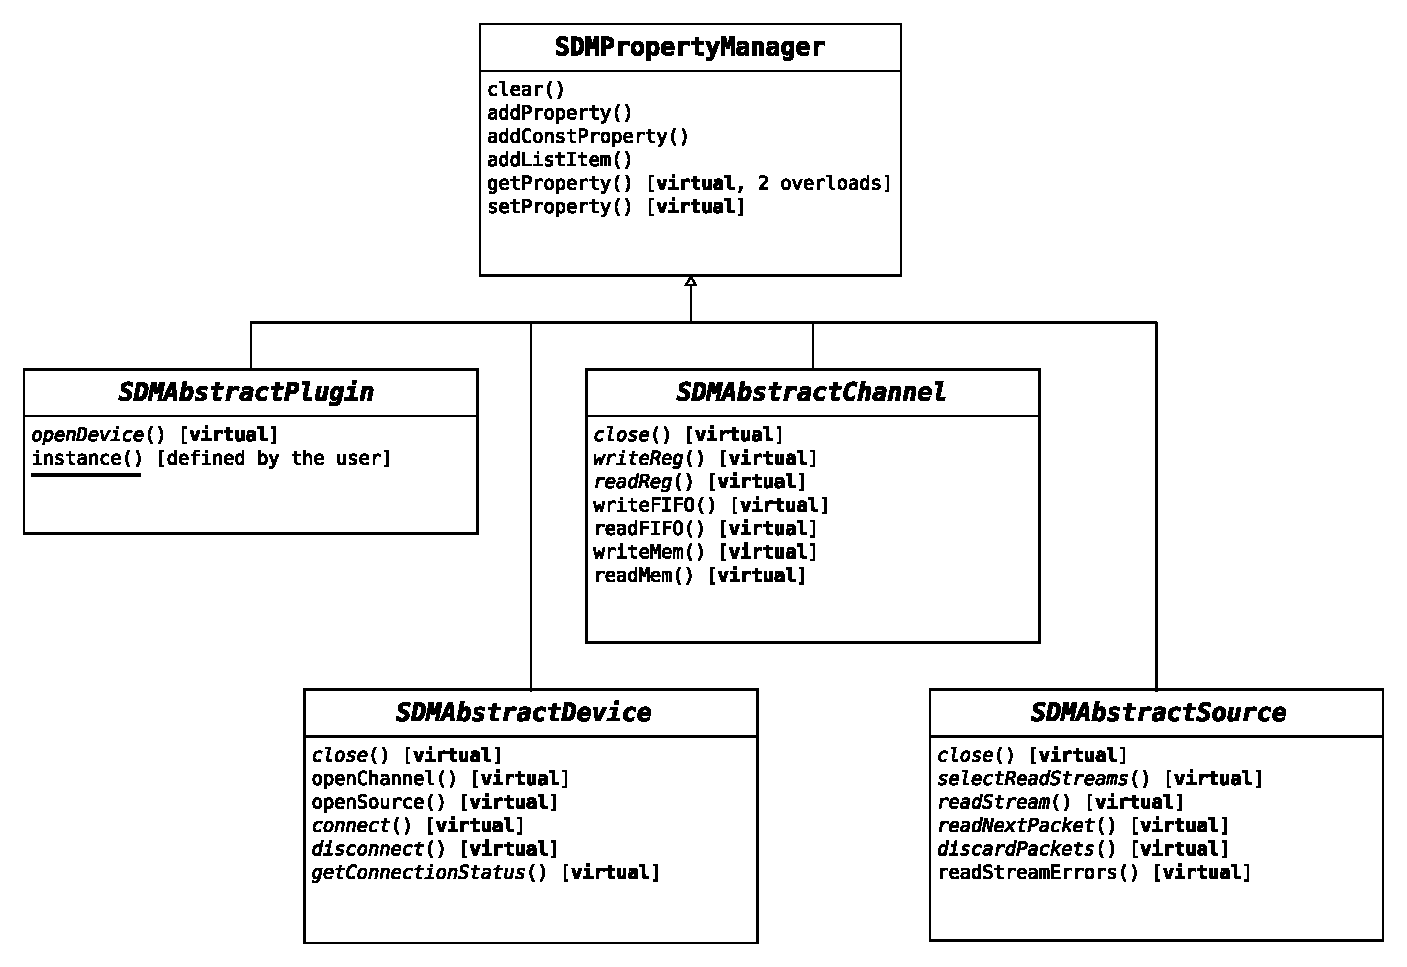
\includegraphics[scale=0.75,angle=90]{images/pluginprovider.pdf}
\caption{\shellcmd{pluginprovider} class diagram}
\label{fig:pluginprovider}
\end{figure}

The \shellcmd{pluginprovider} library is not precompiled, but is provided as a set of source files. This makes it possible to build a plugin with any toolchain, not necessarily the same that was used to build the SDM framework itself.

To create a plugin, include \shellcmd{sdmprovider.h} and perform the following steps:

\begin{enumerate}
	\item Create a plugin class derived from \cexpr{SDMAbstractPlugin}. Override the \cexpr{openDevice()} pure virtual function. Define all the necessary properties using \cexpr{addConstProperty()} for immutable properties and \cexpr{addProperty()} for editable properties; use \cexpr{addListItem()} to create lists.
	\item Provide a definition for the \cexpr{instance()} static member function of the \cexpr{SDMAbstractPlugin} class that returns a pointer to the plugin object instance. It can be done as follows:
\end{enumerate}
	
\begin{breakshellcmds}\begin{ccode}
class TestPlugin : public SDMAbstractPlugin {
// declare TestPlugin members here...
};

SDMAbstractPlugin *SDMAbstractPlugin::instance() {
    static TestPlugin pluginInstance;
    return &pluginInstance;
}
\end{ccode}\end{breakshellcmds}

\begin{enumerate}[label={}]
	\item In the above example a \cexpr{TestPlugin} instance is defined as a static local object. This technique guarantees that \cexpr{instance()} will not return a pointer to an uninitialized object, thus avoiding the situation known as \emph{static initialization order fiasco}.
\end{enumerate}
\begin{enumerate}[start=3]
	\item Derive device, channel and source classes from the respective abstract classes. Override virtual functions and define the necessary properties as above.
	\item Add the \shellcmd{pluginprovider} sources to the build process.
\end{enumerate}

\section{Using SDM with CMake package system}
\label{sec:cmakeconfig}

CMake implements a package system somewhat akin to \emph{pkg-config}. Libraries using CMake as a build system can facilitate integration into downstream projects by providing a configuration package which can be queried to obtain information about libraries and headers location.

SDM configuration package can be loaded using the \shellcmd{find\_package} CMake command. This command makes SDM libraries available as IMPORTED targets with \shellcmd{sdm::} namespace prefix. Libraries exported by SDM are listed in Table \ref{tab:cmaketargets}.

\begin{table}[htbp]
\caption{CMake targets exported by SDM}
\label{tab:cmaketargets}
\begin{tabularx}{\textwidth}{lL}
\toprule
Target & Description \\
\midrule
\shellcmd{sdm::api} & SDM API headers \\
\shellcmd{sdm::pluginprovider} & A \cplusplus{} library for SDM plugin development \\
\shellcmd{sdm::lua} & Lua library, defined only when bundled Lua is used \\
\shellcmd{sdm::ipsockets} & Cross-platform IPv4 sockets library \\ 
\shellcmd{sdm::uart} & Cross-platform serial port library \\
\bottomrule
\end{tabularx}
\end{table}

\shellcmd{sdm::api} is an interface library which does not provide object code, but only adds the directory containing SDM API headers to the list of directories searched for include files.

\shellcmd{sdm::ipsockets} and \shellcmd{sdm::uart} are the \cplusplus{} libraries on which the \shellcmd{luaipsockets} and \shellcmd{luart} bindings are based (see Chapter \ref{ch:scripting}). These libraries are included in the SDK because example plugins depend on them.

For example, \shellcmd{simpleplugin} (see Section \ref{sec:sdmpluginc}) can be built with the following CMake script:

\begin{shellcmds}
cmake\_minimum\_required(VERSION 3.3.0)
project(simpleplugin C)
find\_package(sdm REQUIRED)
add\_library(simpleplugin MODULE simpleplugin.c)
target\_link\_libraries(simpleplugin sdm::api)
set\_target\_properties(simpleplugin PROPERTIES PREFIX "")
\end{shellcmds}

The last line prevents the build system from adding \shellcmd{"lib"} prefix to the output file name when using GCC to ensure consistent plugin naming scheme across all the supported platforms.

For the \shellcmd{find\_package} command to work, CMake must know the location of the \shellcmd{sdm-config.cmake} file. There are multiple ways to do it:

\begin{itemize}
	\item Add the SDM installation prefix to the \shellcmd{CMAKE\_PREFIX\_PATH} CMake variable, or to the environment variable with the same name.
	\item Add the SDM installation prefix to the CMake package registry.
	\item Add the SDM binary directory (Section \ref{sec:installdirectories}) to the \shellcmd{PATH} environment variable.
	\item Include \shellcmd{sdm-config.cmake} directly using the \shellcmd{include} command instead of \shellcmd{find\_package}.
\end{itemize}

More information is available in the CMake documentation, in particular, the \shellcmd{find\_package} command description.

\chapter{Creating applications that use SDM plugins}

\section{Overview}

In order to use code from an SDM plugin, loading it dynamically is not really necessary -- you can just link the plugin code as a static or shared library. If the plugin was created with the \shellcmd{pluginprovider} library, you can even skip the C-style SDM API altogether and access plugin classes directly.

Still, if you want to load a plugin dynamically, SDM sources include reusable code for that purpose. This code is not a part of the SDK. To use it, copy or reference the following libraries to your project and link them to your application:

\begin{alltt}
    sdk/api
    u8e
    utils
    sdmplug
\end{alltt}

In the application itself, include \shellcmd{sdmplug.h} and use the library classes to access the API functions, as in the following example:

\begin{breakshellcmdsnamed}{main.cpp}\begin{ccode}
#include "sdmplug.h"

#include <iostream>

int main() {
// Open plugin objects
	SDMPlugin plugin("./testplugin");
	SDMDevice dev(plugin,0);
	SDMChannel ch(dev,0);
	SDMSource src(dev,0);
	
// Connect the device
	dev.setProperty("Setting1","10.0.0.1");
	dev.setProperty("Setting2","9999");
	dev.connect();
	
// Write/read a register
	std::cout<<"Writing register..."<<std::endl;
	ch.writeReg(10,0x1234);
	std::cout<<"Reading back... "<<ch.readReg(10)<<std::endl;
	
// Read some stream data
	std::vector<int> streams {0};
	src.selectReadStreams(streams,0,1);
	sdm_sample_t buf[10000];
	for(int i=0;i<5;i++) {
		auto samples=src.readStream(0,buf,10000);
		std::cout<<"Reading stream 0 data: ";
		std::cout<<samples<<" samples"<<std::endl;
		src.readNextPacket();
	}
}
\end{ccode}\end{breakshellcmdsnamed}

This example application can be built with the following CMake script:

\begin{shellcmds}
cmake\_minimum\_required(VERSION 3.3.0)
project(sdmtest)
add\_subdirectory(u8e)
add\_subdirectory(api)
add\_subdirectory(utils)
add\_subdirectory(sdmplug)
add\_executable(sdmtest main.cpp)
target\_link\_libraries(sdmtest sdmplug)
\end{shellcmds}

\section{Notes on the SDMPlug library}

SDMPlug class member functions are thin wrappers over the respective SDM API functions and as such are not covered here in detail; refer to Chapter \ref{ch:sdmapireference}.

Plugin paths are assumed to be in UTF-8. If the specified file name does not include an extension, a customary extension for the platform will be appended (\shellcmd{.dll} or \shellcmd{.so}).

Objects owning SDM API handles are reference-counted, so that these handles are not closed until all objects that use them are closed or destroyed. Consider the following example:

\begin{breakshellcmds}\begin{ccode}
SDMDevice dev(plugin,0);
SDMChannel ch(dev,0);
dev.connect();
dev.close();
ch.writereg(10,0x1234);
ch.close();
\end{ccode}\end{breakshellcmds}

Here the \cexpr{dev.close()} statement doesn't result in \cexpr{sdmCloseDevice()} being called since the device is still used by the \cexpr{ch} object. Closing the latter, however, causes the device handle to be closed as well.

\chapter{SDM API reference}
\label{ch:sdmapireference}

\section{Plugin functions}

%%%%%%%%%%%%%%%%%%%%%%%%%%%%%%
% sdmGetPluginProperty()
%%%%%%%%%%%%%%%%%%%%%%%%%%%%%%

\tocitem{subsection}{sdmGetPluginProperty}

\begin{cfuncprototype}
SDMAPI int SDMCALL sdmGetPluginProperty(const char *name, char *buf, size_t n);
\end{cfuncprototype}

\begin{funcdescr}
	Copies the requested plugin property value to the buffer pointed by \cexpr{buf} of size \cexpr{n} bytes.
\end{funcdescr}

\begin{funcparams}
	\funcparam{name}: property name
	\funcparam{buf}: buffer to receive property value, can be \cexpr{NULL} if \cexpr{n=0}
	\funcparam{n}: size of the buffer, can be \cexpr{0}
\end{funcparams}

\begin{funcret}
	If the function succeeds, it returns \cexpr{0}. If the size of buffer is insufficient, it returns the necessary size (including the terminating null character). If the function fails for some other reason (e.g. no property with such name exists), it returns a negative value.
\end{funcret}

%%%%%%%%%%%%%%%%%%%%%%%%%%%%%%
% sdmSetPluginProperty()
%%%%%%%%%%%%%%%%%%%%%%%%%%%%%%

\tocitem{subsection}{sdmSetPluginProperty}

\begin{cfuncprototype}
SDMAPI int SDMCALL sdmSetPluginProperty(const char *name, const char *value);
\end{cfuncprototype}

\begin{funcdescr}
	Sets the plugin property \cexpr{name} to \cexpr{value}.
\end{funcdescr}

\begin{funcparams}
	\funcparam{name}: property name
	\funcparam{value}: property value
\end{funcparams}

\begin{funcret}
	Returns \cexpr{0} if successful, a non-zero value otherwise.
\end{funcret}

\section{Device functions}

%%%%%%%%%%%%%%%%%%%%%%%%%%%%%%
% sdmOpenDevice()
%%%%%%%%%%%%%%%%%%%%%%%%%%%%%%

\tocitem{subsection}{sdmOpenDevice}

\begin{cfuncprototype}
SDMAPI void * SDMCALL sdmOpenDevice(int id);
\end{cfuncprototype}

\begin{funcdescr}
	Opens a device object.
\end{funcdescr}

\begin{funcparams}
	\funcparam{id}: device id (counting from zero)
\end{funcparams}

\begin{funcret}
	Returns a device handle if successful, \cexpr{NULL} otherwise.
\end{funcret}

\begin{funcremarks}
	It is not specified whether a subsequent call to \cexpr{sdmOpenDevice()} with the same \cexpr{id} argument will return a pointer to the same object or a new object. Normally it would be the latter, since it is usually possible to have multiple devices of the same type connected to the same workstation. If \cexpr{sdmOpenDevice()} returns the same pointer, it must still not destroy the device object until \cexpr{sdmCloseDevice()} is called the same number of times.
\end{funcremarks}

%%%%%%%%%%%%%%%%%%%%%%%%%%%%%%
% sdmCloseDevice()
%%%%%%%%%%%%%%%%%%%%%%%%%%%%%%

\tocitem{subsection}{sdmCloseDevice}

\begin{cfuncprototype}
SDMAPI int SDMCALL sdmCloseDevice(void *h);
\end{cfuncprototype}

\begin{funcdescr}
	Closes the device object.
\end{funcdescr}

\begin{funcparams}
	\funcparam{h}: device handle
\end{funcparams}

\begin{funcret}
	Returns \cexpr{0} if successful, a non-zero value otherwise.
\end{funcret}

\begin{funcremarks}
	Note: don't close the device when there are still channels or sources opened on this device.
\end{funcremarks}

%%%%%%%%%%%%%%%%%%%%%%%%%%%%%%
% sdmGetDeviceProperty()
%%%%%%%%%%%%%%%%%%%%%%%%%%%%%%

\tocitem{subsection}{sdmGetDeviceProperty}

\begin{cfuncprototype}
SDMAPI int SDMCALL sdmGetDeviceProperty(void *h, const char *name, char *buf, size_t n);
\end{cfuncprototype}

\begin{funcdescr}
	Copies the requested device property value to the buffer pointed by \cexpr{buf} of size \cexpr{n} bytes.
\end{funcdescr}

\begin{funcparams}
	\funcparam{h}: device handle
	\funcparam{buf}: buffer to receive property value, can be \cexpr{NULL} if \cexpr{n=0}
	\funcparam{n}: size of the buffer, can be \cexpr{0}
\end{funcparams}

\begin{funcret}
	As in \expr{sdmGetPluginProperty}.
\end{funcret}

%%%%%%%%%%%%%%%%%%%%%%%%%%%%%%
% sdmSetDeviceProperty()
%%%%%%%%%%%%%%%%%%%%%%%%%%%%%%

\tocitem{subsection}{sdmSetDeviceProperty}

\begin{cfuncprototype}
SDMAPI int SDMCALL sdmSetDeviceProperty(void *h, const char *name, const char *value);
\end{cfuncprototype}

\begin{funcdescr}
	Sets the device property \cexpr{name} to \cexpr{value}.
\end{funcdescr}

\begin{funcparams}
	\funcparam{h}: device handle
	\funcparam{name}: property name
	\funcparam{value}: property value
\end{funcparams}

\begin{funcret}
	Returns \cexpr{0} if successful, a non-zero value otherwise.
\end{funcret}

%%%%%%%%%%%%%%%%%%%%%%%%%%%%%%
% sdmConnect()
%%%%%%%%%%%%%%%%%%%%%%%%%%%%%%

\tocitem{subsection}{sdmConnect}

\begin{cfuncprototype}
SDMAPI int SDMCALL sdmConnect(void *h);
\end{cfuncprototype}

\begin{funcdescr}
	Connects to the remote device.
\end{funcdescr}

\begin{funcparams}
	\funcparam{h}: device handle
\end{funcparams}

\begin{funcret}
	Returns \cexpr{0} if successful, a non-zero value otherwise.
\end{funcret}

\begin{funcremarks}
	If a device requires connection parameters, they are set using the device object's property interface.
\end{funcremarks}

%%%%%%%%%%%%%%%%%%%%%%%%%%%%%%
% sdmDisconnect()
%%%%%%%%%%%%%%%%%%%%%%%%%%%%%%

\tocitem{subsection}{sdmDisconnect}

\begin{cfuncprototype}
SDMAPI int SDMCALL sdmDisconnect(void *h);
\end{cfuncprototype}

\begin{funcdescr}
	Disconnects from the remote device.
\end{funcdescr}

\begin{funcparams}
	\funcparam{h}: device handle
\end{funcparams}

\begin{funcret}
	Returns \cexpr{0} if successful, a non-zero value otherwise.
\end{funcret}

%%%%%%%%%%%%%%%%%%%%%%%%%%%%%%
% sdmGetConnectionStatus()
%%%%%%%%%%%%%%%%%%%%%%%%%%%%%%

\tocitem{subsection}{sdmGetConnectionStatus}

\begin{cfuncprototype}
SDMAPI int SDMCALL sdmGetConnectionStatus(void *h);
\end{cfuncprototype}

\begin{funcdescr}
	Queries the device connection status.
\end{funcdescr}

\begin{funcparams}
	\funcparam{h}: device handle
\end{funcparams}

\begin{funcret}
	Returns a non-zero value for an active connection, zero otherwise.
\end{funcret}

\section{Channel functions}
\label{sec:channelfunctions}

%%%%%%%%%%%%%%%%%%%%%%%%%%%%%%
% sdmOpenChannel()
%%%%%%%%%%%%%%%%%%%%%%%%%%%%%%

\tocitem{subsection}{sdmOpenChannel}

\begin{cfuncprototype}
SDMAPI void * SDMCALL sdmOpenChannel(void *hdev, int id);
\end{cfuncprototype}

\begin{funcdescr}
	Opens a channel object.
\end{funcdescr}

\begin{funcparams}
	\funcparam{hdev}: device handle
	\funcparam{id}: channel id (counting from zero)
\end{funcparams}

\begin{funcret}
	Returns a channel handle if successful, \cexpr{NULL} otherwise.
\end{funcret}

\begin{funcremarks}
	It is not specified whether a subsequent call to \cexpr{sdmOpenChannel()} with the same \cexpr{id} argument will return a pointer to the same object or a new object. If \cexpr{sdmOpenChannel()} returns the same pointer, it must still not destroy the object until \cexpr{sdmCloseChannel()} is called the same number of times.
\end{funcremarks}

%%%%%%%%%%%%%%%%%%%%%%%%%%%%%%
% sdmCloseChannel()
%%%%%%%%%%%%%%%%%%%%%%%%%%%%%%

\tocitem{subsection}{sdmCloseChannel}

\begin{cfuncprototype}
SDMAPI int SDMCALL sdmCloseChannel(void *h);
\end{cfuncprototype}

\begin{funcdescr}
	Closes the channel object.
\end{funcdescr}

\begin{funcparams}
	\funcparam{h}: channel handle
\end{funcparams}

\begin{funcret}
	Returns \cexpr{0} if successful, a non-zero value otherwise.
\end{funcret}

%%%%%%%%%%%%%%%%%%%%%%%%%%%%%%
% sdmGetChannelProperty()
%%%%%%%%%%%%%%%%%%%%%%%%%%%%%%

\tocitem{subsection}{sdmGetChannelProperty}

\begin{cfuncprototype}
SDMAPI int SDMCALL sdmGetChannelProperty(void *h, const char *name, char *buf, size_t n);
\end{cfuncprototype}

\begin{funcdescr}
	Copies the requested channel property value to the buffer pointed by \cexpr{buf} of size \cexpr{n} bytes.
\end{funcdescr}

\begin{funcparams}
	\funcparam{h}: channel handle
	\funcparam{buf}: buffer to receive property value, can be \cexpr{NULL} if \cexpr{n=0}
	\funcparam{n}: size of the buffer, can be \cexpr{0}
\end{funcparams}

\begin{funcret}
	As in \expr{sdmGetPluginProperty}.
\end{funcret}

%%%%%%%%%%%%%%%%%%%%%%%%%%%%%%
% sdmSetChannelProperty()
%%%%%%%%%%%%%%%%%%%%%%%%%%%%%%

\tocitem{subsection}{sdmSetChannelProperty}

\begin{cfuncprototype}
SDMAPI int SDMCALL sdmSetChannelProperty(void *h, const char *name, const char *value);
\end{cfuncprototype}

\begin{funcdescr}
	Sets the channel property \cexpr{name} to \cexpr{value}.
\end{funcdescr}

\begin{funcparams}
	\funcparam{h}: channel handle
	\funcparam{name}: property name
	\funcparam{value}: property value
\end{funcparams}

\begin{funcret}
	Returns \cexpr{0} if successful, a non-zero value otherwise.
\end{funcret}

%%%%%%%%%%%%%%%%%%%%%%%%%%%%%%
% sdmWriteReg()
%%%%%%%%%%%%%%%%%%%%%%%%%%%%%%

\tocitem{subsection}{sdmWriteReg}

\begin{cfuncprototype}
SDMAPI int SDMCALL sdmWriteReg(void *h, sdm_addr_t addr, sdm_reg_t data);
\end{cfuncprototype}

\begin{funcdescr}
	Writes to a register. This function is blocking.
\end{funcdescr}

\begin{funcparams}
	\funcparam{h}: channel handle
	\funcparam{addr}: register address
	\funcparam{data}: data to write
\end{funcparams}

\begin{funcret}
	Returns \cexpr{0} if successful, a non-zero value otherwise.
\end{funcret}

%%%%%%%%%%%%%%%%%%%%%%%%%%%%%%
% sdmReadReg()
%%%%%%%%%%%%%%%%%%%%%%%%%%%%%%

\tocitem{subsection}{sdmReadReg}

\begin{cfuncprototype}
SDMAPI sdm_reg_t SDMCALL sdmReadReg(void *h, sdm_addr_t addr, int *status);
\end{cfuncprototype}

\begin{funcdescr}
	Reads from a register. This function is blocking.
\end{funcdescr}

\begin{funcparams}
	\funcparam{h}: channel handle
	\funcparam{addr}: register address
	\funcparam{status}: pointer to a variable to receive operation success status, can be \cexpr{NULL}
\end{funcparams}

\begin{funcret}
	If successful, returns the value read from the register. If \cexpr{status} is not \cexpr{NULL}, sets \cexpr{*status} to \cexpr{0} in case of success and to a non-zero value otherwise.
\end{funcret}

%%%%%%%%%%%%%%%%%%%%%%%%%%%%%%
% sdmWriteFIFO()
%%%%%%%%%%%%%%%%%%%%%%%%%%%%%%

\tocitem{subsection}{sdmWriteFIFO}

\begin{cfuncprototype}
SDMAPI int SDMCALL sdmWriteFIFO(void *h, sdm_addr_t addr, const sdm_reg_t *data, size_t n, int flags);
\end{cfuncprototype}

\begin{funcdescr}
	Writes an array of words to a FIFO. This function is blocking.
\end{funcdescr}

\begin{funcparams}
	\funcparam{h}: channel handle
	\funcparam{addr}: register address
	\funcparam{data}: pointer to an array of words to write
	\funcparam{n}: number of words to write
	\funcparam{flags}: reserved, must be set to zero
\end{funcparams}

\begin{funcret}
	Returns a non-negative value if successful, a negative value otherwise. Note: it used to be required that this function returns the number of words written, but it is no longer necessary.
\end{funcret}

\begin{funcremarks}
	FIFO represents a memory block that is mapped to a single register address. Writing to a FIFO is conceptually equivalent to performing a set of ordinary register writes in sequence, but can be more efficient for devices supporting block transactions.
\end{funcremarks}

%%%%%%%%%%%%%%%%%%%%%%%%%%%%%%
% sdmReadFIFO()
%%%%%%%%%%%%%%%%%%%%%%%%%%%%%%

\tocitem{subsection}{sdmReadFIFO}

\begin{cfuncprototype}
SDMAPI int SDMCALL sdmReadFIFO(void *h, sdm_addr_t addr, sdm_reg_t *data, size_t n, int flags);
\end{cfuncprototype}

\begin{funcdescr}
	Reads an array of words from a FIFO. This function is blocking.
\end{funcdescr}

\begin{funcparams}
	\funcparam{h}: channel handle
	\funcparam{addr}: register address
	\funcparam{data}: pointer to an array to read to
	\funcparam{n}: number of words to read
	\funcparam{flags}: reserved, must be set to zero
\end{funcparams}

\begin{funcret}
	Returns a non-negative value if successful, a negative value otherwise. Note: it used to be required that this function returns the number of words read, but it is no longer necessary.
\end{funcret}

\begin{funcremarks}
	FIFO represents a memory block that is mapped to a single register address. Reading from a FIFO is conceptually equivalent to performing a set of ordinary register reads in sequence, but can be more efficient for devices supporting block transactions.
\end{funcremarks}

%%%%%%%%%%%%%%%%%%%%%%%%%%%%%%
% sdmWriteMem()
%%%%%%%%%%%%%%%%%%%%%%%%%%%%%%

\tocitem{subsection}{sdmWriteMem}

\begin{cfuncprototype}
SDMAPI int SDMCALL sdmWriteMem(void *h, sdm_addr_t addr, const sdm_reg_t *data, size_t n);
\end{cfuncprototype}

\begin{funcdescr}
	Writes an array of words to a memory block starting at \cexpr{addr}. This function is blocking.
\end{funcdescr}

\begin{funcparams}
	\funcparam{h}: channel handle
	\funcparam{addr}: register address
	\funcparam{data}: pointer to an array to write
	\funcparam{n}: number of words to write
\end{funcparams}

\begin{funcret}
	Returns \cexpr{0} if successful, a non-zero value otherwise.
\end{funcret}

\begin{funcremarks}
	Writing to memory is conceptually equivalent to performing a set of register writes with incrementing addresses, but can be more efficient for devices supporting block transactions. Depending on address granularity, the address can be incremented by a value other than 1.
\end{funcremarks}

%%%%%%%%%%%%%%%%%%%%%%%%%%%%%%
% sdmReadMem()
%%%%%%%%%%%%%%%%%%%%%%%%%%%%%%

\tocitem{subsection}{sdmReadMem}

\begin{cfuncprototype}
SDMAPI int SDMCALL sdmReadMem(void *h, sdm_addr_t addr, sdm_reg_t *data, size_t n);
\end{cfuncprototype}

\begin{funcdescr}
	Reads an array of words from a memory block starting at \cexpr{addr}. This function is blocking.
\end{funcdescr}

\begin{funcparams}
	\funcparam{h}: channel handle
	\funcparam{addr}: register address
	\funcparam{data}: pointer to an array to store read data
	\funcparam{n}: number of words to read
\end{funcparams}

\begin{funcret}
	Returns \cexpr{0} if successful, a non-zero value otherwise.
\end{funcret}

\begin{funcremarks}
	Reading from memory is conceptually equivalent to performing a set of register reads with incrementing addresses, but can be more efficient for devices supporting block transactions. Depending on address granularity, the address can be incremented by a value other than 1.
\end{funcremarks}

\section{Source functions}
\label{sec:sourcefunctions}

%%%%%%%%%%%%%%%%%%%%%%%%%%%%%%
% sdmOpenSource()
%%%%%%%%%%%%%%%%%%%%%%%%%%%%%%

\tocitem{subsection}{sdmOpenSource}

\begin{cfuncprototype}
SDMAPI void * SDMCALL sdmOpenSource(void *hdev, int id);
\end{cfuncprototype}

\begin{funcdescr}
	Opens a source object.
\end{funcdescr}

\begin{funcparams}
	\funcparam{hdev}: device handle
	\funcparam{id}: source id (counting from zero)
\end{funcparams}

\begin{funcret}
	Returns a source handle if successful, \cexpr{NULL} otherwise.
\end{funcret}

\begin{funcremarks}
	It is not specified whether a subsequent call to \cexpr{sdmOpenSource()} with the same \cexpr{id} argument will return a pointer to the same object or a new object. If \cexpr{sdmOpenSource()} returns the same pointer, it must still not destroy the object until \cexpr{sdmCloseSource()} is called the same number of times.
\end{funcremarks}

%%%%%%%%%%%%%%%%%%%%%%%%%%%%%%
% sdmCloseSource()
%%%%%%%%%%%%%%%%%%%%%%%%%%%%%%

\tocitem{subsection}{sdmCloseSource}

\begin{cfuncprototype}
SDMAPI int SDMCALL sdmCloseSource(void *h);
\end{cfuncprototype}

\begin{funcdescr}
	Closes the source object.
\end{funcdescr}

\begin{funcparams}
	\funcparam{h}: source handle
\end{funcparams}

\begin{funcret}
	Returns \cexpr{0} if successful, a non-zero value otherwise.
\end{funcret}

%%%%%%%%%%%%%%%%%%%%%%%%%%%%%%
% sdmGetSourceProperty()
%%%%%%%%%%%%%%%%%%%%%%%%%%%%%%

\tocitem{subsection}{sdmGetSourceProperty}

\begin{cfuncprototype}
SDMAPI int SDMCALL sdmGetSourceProperty(void *h, const char *name, char *buf, size_t n);
\end{cfuncprototype}

\begin{funcdescr}
	Copies the requested source property value to the buffer pointed by \cexpr{buf} of size \cexpr{n} bytes.
\end{funcdescr}

\begin{funcparams}
	\funcparam{h}: source handle
	\funcparam{buf}: buffer to receive property value, can be \cexpr{NULL} if \cexpr{n=0}
	\funcparam{n}: size of the buffer, can be \cexpr{0}
\end{funcparams}

\begin{funcret}
	As in \expr{sdmGetPluginProperty}.
\end{funcret}

%%%%%%%%%%%%%%%%%%%%%%%%%%%%%%
% sdmSetSourceProperty()
%%%%%%%%%%%%%%%%%%%%%%%%%%%%%%

\tocitem{subsection}{sdmSetSourceProperty}

\begin{cfuncprototype}
SDMAPI int SDMCALL sdmSetSourceProperty(void *h, const char *name, const char *value);
\end{cfuncprototype}

\begin{funcdescr}
	Sets the source property \cexpr{name} to \cexpr{value}.
\end{funcdescr}

\begin{funcparams}
	\funcparam{h}: source handle
	\funcparam{name}: property name
	\funcparam{value}: property value
\end{funcparams}

\begin{funcret}
	Returns \cexpr{0} if successful, a non-zero value otherwise.
\end{funcret}

%%%%%%%%%%%%%%%%%%%%%%%%%%%%%%
% sdmSelectReadStreams()
%%%%%%%%%%%%%%%%%%%%%%%%%%%%%%

\tocitem{subsection}{sdmSelectReadStreams}

\begin{cfuncprototype}
SDMAPI int SDMCALL sdmSelectReadStreams(void *h, const int *streams, size_t n, size_t packets, int df);
\end{cfuncprototype}

\begin{funcdescr}
	Selects data streams for reading.
\end{funcdescr}

\begin{funcparams}
	\funcparam{h}: source handle
	\funcparam{streams}: pointer to an array of stream ids
	\funcparam{n}: size of the array, can be \cexpr{0}
	\funcparam{packets}: suggested minimum number of packets to deliver consecutively (per stream), \cexpr{0} for default (see the Remarks below)
	\funcparam{df}: suggested decimation factor, \cexpr{1} or greater, see the Remarks below
\end{funcparams}

\begin{funcret}
	Returns \cexpr{0} if successful, a non-zero value otherwise.
\end{funcret}

\begin{funcremarks}
	The \cexpr{streams} argument is ignored when \cexpr{n=0} (no streams are selected).
	
	A non-zero \cexpr{packets} value is a non-binding request to deliver at least the specified number of consecutive packets after this function is called (for streams that don't support the notion of packets, this argument is interpreted as a number of samples). This information can be used by the plugin, for example, to allocate a buffer of suitable size. The plugin is not required to honor this argument.
	
	A \cexpr{df} argument value greater than 1 is a non-binding request to reduce the source output bandwidth by the factor of \cexpr{df}. How the decimation is performed, if at all, is up to the implementation: for example, it can deliver only one of each \cexpr{df} packets, or deliver all packets, but only one of each \cexpr{df} samples in each packet. For high-bandwidth data sources that generate too much data to be processed in real time, it gives the user a choice: either receive decimated data in real time (e.g. for visualisation), or receive complete data for a limited duration (until the buffer is full). This implies some kind of data buffering by the device.
	
	If the stream supports the notion of packets, the next read operation after this function has been called will read from the start of the packet.
	
	Calling this function resets the stream error counter.
\end{funcremarks}

%%%%%%%%%%%%%%%%%%%%%%%%%%%%%%
% sdmReadStream
%%%%%%%%%%%%%%%%%%%%%%%%%%%%%%

\tocitem{subsection}{sdmReadStream}

\begin{cfuncprototype}
SDMAPI int SDMCALL sdmReadStream(void *h, int stream, sdm_sample_t *data, size_t n, int nb);
\end{cfuncprototype}

\begin{funcdescr}
	Reads data from a stream.
\end{funcdescr}

\begin{funcparams}
	\funcparam{h}: source handle
	\funcparam{stream}: stream id
	\funcparam{data}: pointer to an array to receive data
	\funcparam{n}: size of the array
	\funcparam{nb}: a non-zero value indicates a non-blocking operation request
\end{funcparams}

\begin{funcret}
	In the blocking mode: number of samples read (\cexpr{0} at the end of packet). Negative value indicates an error. It is not an error when number of bytes read is less than requested.
	
	In the non-blocking mode: as above, plus \cexpr{SDM_WOULDBLOCK} if no data
	are available for non-blocking reading.
	
	In addition to the above, if \cexpr{n} is \cexpr{0}, the functions returns \cexpr{0}.
\end{funcret}

\begin{funcremarks}
	In the blocking mode, the function returns when either (1) the requested number of samples has been read, (2) at least one sample has been read and no more data are available for immediate reading, (3) packet ends or (4) an error occurs. In the non-blocking mode, in addition to the above conditions, the function returns when there are no data available for immediate reading.
	
	The requested stream must be selected with \cexpr{sdmSelectReadStreams()}. The function reads the next data chunk from the stream buffer. To continue reading after the current packet ends, \cexpr{sdmReadNextPacket()} must be called. If several streams were selected, the respective packets are guaranteed to be delivered synchronously.
	
	The concept of packets is important for stream synchronization if the source has more than one stream. Until \cexpr{sdmReadNextPacket()} is called, data read from any stream are implied to have been captured at the same time. Packets in different streams can have different sizes. If the stream data aren't inherently packetized, it is still strongly recommended to divide samples into packets for the purpose of synchronization and data visualization.
\end{funcremarks}

%%%%%%%%%%%%%%%%%%%%%%%%%%%%%%
% sdmReadNextPacket
%%%%%%%%%%%%%%%%%%%%%%%%%%%%%%

\tocitem{subsection}{sdmReadNextPacket}

\begin{cfuncprototype}
SDMAPI int SDMCALL sdmReadNextPacket(void *h);
\end{cfuncprototype}

\begin{funcdescr}
	Proceeds to the next packet. This function affects all streams. Any unread data from the current packet are discarded.
\end{funcdescr}

\begin{funcparams}
	\funcparam{h}: source handle
\end{funcparams}

\begin{funcret}
	Returns \cexpr{0} if successful, a non-zero value otherwise.
\end{funcret}

\begin{funcremarks}
	If no streams are selected, or the source doesn't support the notion of packets, calling this function has no effect.
\end{funcremarks}

%%%%%%%%%%%%%%%%%%%%%%%%%%%%%%
% sdmDiscardPackets()
%%%%%%%%%%%%%%%%%%%%%%%%%%%%%%

\tocitem{subsection}{sdmDiscardPackets}

\begin{cfuncprototype}
SDMAPI void SDMCALL sdmDiscardPackets(void *h);
\end{cfuncprototype}

\begin{funcdescr}
	Discards all data currently buffered for stream reading. If the source supports the notion of packets, the next read operation will read data from the beginning of the first packet that was added to the buffer after this function was called.
\end{funcdescr}

\begin{funcparams}
	\funcparam{h}: source handle
\end{funcparams}

\begin{funcremarks}
	This function resets the stream error counter.
\end{funcremarks}

%%%%%%%%%%%%%%%%%%%%%%%%%%%%%%
% sdmReadStreamErrors()
%%%%%%%%%%%%%%%%%%%%%%%%%%%%%%

\tocitem{subsection}{sdmReadStreamErrors}

\begin{cfuncprototype}
SDMAPI int SDMCALL sdmReadStreamErrors(void *h);
\end{cfuncprototype}

\begin{funcdescr}
	Gets a number of stream errors for the source.
\end{funcdescr}

\begin{funcparams}
	\funcparam{h}: source handle
\end{funcparams}

\begin{funcret}
	Returns the value of a stream error counter.
\end{funcret}

\begin{funcremarks}
	A stream error is a condition when consecutive operations read non-consecutive data, possibly because of a packet loss or a receiver buffer overflow.
\end{funcremarks}

\appendix

\chapter{Command line syntax}
\label{app:cmdline}

\section[sdmhost]{\shellcmd{sdmhost}}

\begin{shellcmds}
sdmhost
\end{shellcmds}

Run \shellcmd{sdmhost} in interactive mode, reading commands from standard input.

\begin{shellcmds}
sdmhost \emph{filename} [ \emph{scriptargs} ]
\end{shellcmds}

Execute a script from the \shellcmd{\emph{filename}} and exit.

\begin{shellcmds}
sdmhost -i \emph{filename} [ \emph{scriptargs} ]
\end{shellcmds}

Execute a script from the \shellcmd{\emph{filename}}, then enter interactive mode.

\begin{shellcmds}
sdmhost -h
sdmhost --help
\end{shellcmds}

Display a short help message.

Script arguments, per Lua custom, are passed in the \luaexpr{arg} global table. The first script argument has index \luaexpr{1}. Previous command line arguments have indexes \luaexpr{0} and below.

\section[sdmconsole]{\shellcmd{sdmconsole}}

\begin{shellcmds}
sdmconsole [ arguments ]
\end{shellcmds}

Run \shellcmd{sdmconsole}. Optional arguments:

\begin{itemize}
	\item \shellcmd{--run \emph{filename} [ \emph{scriptargs} ]} -- execute a script. Must be the last argument (further arguments are passed to the script via the \luaexpr{arg} table, as in \shellcmd{sdmhost}).
	\item \shellcmd{--batch \emph{filename} [ \emph{scriptargs} ]} -- execute a script and exit if there were no errors.
\end{itemize}

Debug options (should not be used normally):

\begin{itemize}
	\item \shellcmd{--no-redirector} -- disable standard output redirection. Lua console will not work properly with this option.
	\item \shellcmd{--alt-redirector} -- under Windows, use alternative standard output redirection method. The alternative method is less intrusive, but also less reliable than the default one. Under Linux this option is ignored.
\end{itemize}

\chapter{MHDB 1.2 file format}
\label{app:mhdbformat}

\section{Overview}

MHDB file format is used by \shellcmd{sdmconsole} to store the captured data streams. It supports multiple channels and high dynamic range samples. MHDB requires a constant packet (line) size and will not be able to store streams with variable packet size. The file consists of three parts:

\begin{itemize}
	\item Header,
	\item Metadata,
	\item Payload.
\end{itemize}

Metadata block is optional and can be absent.

MHDB uses little-endian format to represent multi-byte values.

\section{File header}

The file header has a fixed size of 32 bytes. Its structure is shown in table \ref{tab:mhdbheader}.

\begin{table}[htbp]
\caption{MHDB header}
\label{tab:mhdbheader}
\def\arraystretch{1.2}
\begin{tabularx}{\textwidth}{|p{6em}|C|C|C|C|}
\hline
\multirow{2}{6em}{Offset (bytes)} & \multicolumn{4}{c|}{Bits} \\
\cline{2-5}
 & 0--7 & 8--15 & 16--23 & 24--31 \\
\hline
0 & \multicolumn{4}{c|}{SIGNATURE} \\
\hline
4 & \multicolumn{4}{c|}{NLINES} \\
\hline
8 & \multicolumn{4}{c|}{NSAMPLES\_PER\_LINE} \\
\hline
12 & CHANNELS & DIGITS & BPS & VERSION \\
\hline
16 & \multicolumn{2}{c|}{META\_SIZE} & STYPE & \emph{reserved} \\
\hline
20 & \multicolumn{4}{c|}{} \\
24 & \multicolumn{4}{c|}{\emph{reserved}} \\
28 & \multicolumn{4}{c|}{} \\
\hline
\end{tabularx}
\end{table}

The header contains the following fields:

\begin{itemize}
	\item SIGNATURE -- \texttt{MHDB} signature.
	\item NLINES -- number of lines in the file (per channel).
	\item NSAMPLES\_PER\_LINE -- number of samples per line.
	\item CHANNELS -- number of channels (1--255).
	\item DIGITS -- number of significant bits per sample ($\le$~8~$\cdot$~BPS for integral sample formats, $=$~8~$\cdot$~BPS for floating point sample formats).
	\item BPS -- number of bytes per sample, together with STYPE determines the sample format (see the subsection \ref{subsec:mhdbsampleformat} below).
	\item VERSION -- file format version (upper 4 bits -- major version number, lower 4 bits -- minor version number). The current version (1.2) is represented as 0x12.
	\item META\_SIZE -- size of metadata block, in bytes. Must be multiple of 4, can be zero.
	\item STYPE -- sample type, together with BPS determines the sample format (see the subsection \ref{subsec:mhdbsampleformat} below).
\end{itemize}

Reserved header fields must be filled with zeros. Contents of the metadata block are not specified.

\section{Payload}

The payload consists of lines. Each line is prepended with the 4-byte line header. Lines that were received simultaneously from multiple channels are written sequentially in the ascending order of channel numbers. The total line size in bytes (including header):

\begin{center}
	NSAMPLES\textunderscore PER\textunderscore LINE $\cdot$ BPS+4
\end{center}

\subsection{Line header}

\begin{table}[htbp]
\caption{MHDB line header format}
\label{tab:mhdblineheader}
\small
\def\arraystretch{1.2}
\begin{tabularx}{\textwidth}{|p{6em}|C|C|C|C|}
\hline
\multirow{2}{6em}{Offset (bytes)} & \multicolumn{4}{c|}{Bits} \\
\cline{2-5}
 & 0--7 & 8--15 & 16--23 & 24--31 \\
\hline
0 & \multicolumn{3}{c|}{SEQ} & CH \\
\hline
\end{tabularx}
\end{table}

Line header format is shown in table \ref{tab:mhdblineheader}. Line header contains the following fields:

\begin{itemize}
	\item SEQ --  line number, counting from 0. Lines that are received simultaneously (from different channels) have the same number.
	\item CH -- channel number, counting from 0.
\end{itemize}

\subsection{Sample format}
\label{subsec:mhdbsampleformat}

The line header is followed by data samples. Number of samples is determined by the NSAMPLES\_PER\_LINE field of the file header. The sample format is determined by BPS and STYPE fields. Supported formats are listed in table \ref{tab:mhdbsampleformat}.

\begin{table}[htbp]
\caption{Supported MHDB sample formats}
\label{tab:mhdbsampleformat}
\begin{tabularx}{\textwidth}{llL}
\toprule
BPS & STYPE & Format \\
\midrule
1 & 0 & 8-bit unsigned integer \\
1 & 1 & 8-bit signed integer \\
2 & 0 & 16-bit unsigned integer \\
2 & 1 & 16-bit signed integer \\
4 & 0 & 32-bit unsigned integer \\
4 & 1 & 32-bit signed integer \\
4 & 2 & 32-bit floating point (single precision) \\
8 & 0 & 64-bit unsigned integer \\
8 & 1 & 64-bit signed integer \\
8 & 2 & 64-bit floating point (double precision) \\
\bottomrule
\end{tabularx}
\end{table}

\end{document}
